% ==================================================================
% TEMPLATE TCC MACKENZIE - BRUNO GASPARONI BALLERINI
% Baseado nas normas do Guia do TCC 2022 - Universidade Presbiteriana Mackenzie
% ==================================================================

\documentclass[12pt,a4paper,oneside]{report}

% ==================================================================
% PACOTES NECESSÁRIOS
% ==================================================================
\usepackage[utf8]{inputenc}
\usepackage[T1]{fontenc}
\usepackage[portuguese]{babel}
\usepackage{mathptmx} % Times New Roman
\usepackage{setspace}
\usepackage{geometry}
\usepackage{titlesec}
\usepackage{tocloft}
\usepackage{fancyhdr}
\usepackage{graphicx}
\usepackage{amsmath}
\usepackage{amsfonts}
\usepackage{amssymb}
\usepackage{indentfirst}
\usepackage{caption}
\usepackage{subcaption}
\usepackage{float}
\usepackage[hidelinks]{hyperref}
\usepackage{url}
\usepackage{booktabs}
\usepackage{array}
\usepackage{multirow}
\usepackage{longtable}

% ==================================================================
% CONFIGURAÇÕES GERAIS MACKENZIE
% ==================================================================

% Margens: 3cm (superior e esquerda), 2cm (inferior e direita)
\geometry{
    a4paper,
    top=3cm,
    left=3cm,
    bottom=2cm,
    right=2cm
}

% Espaçamento 1.5
\onehalfspacing

% Recuo de parágrafo 1,25cm
\setlength{\parindent}{1.25cm}

% Espaçamento entre parágrafos - SEM espaço extra (conforme guia p.40)
\setlength{\parskip}{0pt}

% ==================================================================
% CONFIGURAÇÃO DE TÍTULOS (NORMAS MACKENZIE)
% ==================================================================

% Seção primária: 1 LETRAS MAIÚSCULAS EM NEGRITO  
\titleformat{\chapter}[hang]
{\normalfont\fontsize{12}{14.4}\bfseries}
{\thechapter}{1em}{\MakeUppercase}
\titlespacing*{\chapter}{0pt}{0pt}{12pt}

% Títulos de capítulos não numerados (centralizados)
\titleformat{name=\chapter,numberless}[block]
{\normalfont\fontsize{12}{14.4}\bfseries\centering}
{}{0pt}{\MakeUppercase}
\titlespacing*{name=\chapter,numberless}{0pt}{0pt}{12pt}

% Seção secundária: 1.1 LETRAS MAIÚSCULAS SEM NEGRITO
\titleformat{\section}[hang]
{\normalfont\fontsize{12}{14.4}}
{\thesection}{1em}{\MakeUppercase}
\titlespacing*{\section}{0pt}{\baselineskip}{\baselineskip}

% Seção terciária: 1.1.1 Letras minúsculas em negrito
\titleformat{\subsection}[hang]
{\normalfont\fontsize{12}{14.4}\bfseries}
{\thesubsection}{1em}{}
\titlespacing*{\subsection}{0pt}{12pt}{12pt}

% Seção quaternária: 1.1.1.1 Letras minúsculas sem negrito
\titleformat{\subsubsection}[hang]
{\normalfont\fontsize{12}{14.4}}
{\thesubsubsection}{1em}{}
\titlespacing*{\subsubsection}{0pt}{12pt}{12pt}

% Seção quinária: 1.1.1.1.1 Letras minúsculas em itálico
\titleformat{\paragraph}[hang]
{\normalfont\fontsize{12}{14.4}\itshape}
{\theparagraph}{1em}{}
\titlespacing*{\paragraph}{0pt}{12pt}{12pt}

% ==================================================================
% NUMERAÇÃO DE PÁGINAS
% ==================================================================
\setlength{\headheight}{13.19998pt}
\pagestyle{fancy}
\fancyhf{}
% Numeração a 2cm das bordas superior e direita
\fancyhead[R]{\fontsize{11}{13.2}\selectfont\thepage}
\fancyheadoffset{0cm}
\renewcommand{\headrulewidth}{0pt}

% ==================================================================
% CONFIGURAÇÃO DO SUMÁRIO
% ==================================================================
\renewcommand{\contentsname}{SUMÁRIO}
\renewcommand{\cftchapfont}{\fontsize{12}{14.4}\selectfont\bfseries}
\renewcommand{\cftsecfont}{\fontsize{12}{14.4}\selectfont}
\renewcommand{\cftsubsecfont}{\fontsize{12}{14.4}\selectfont}
\renewcommand{\cftchapleader}{\cftdotfill{\cftdotsep}}
\setlength{\cftbeforechapskip}{6pt}

% ==================================================================
% INÍCIO DO DOCUMENTO
% ==================================================================
\begin{document}

% CAPA - sem numeração
\pagenumbering{gobble}
% ==================================================================
% CAPA - CONFORME MODELO MACKENZIE (Apêndice D do Guia)
% ==================================================================

\thispagestyle{empty}

\begin{center}

% Espaçamento superior
\vspace*{3cm}

% Nome da instituição
{\fontsize{12}{14.4}\selectfont\bfseries\MakeUppercase{UNIVERSIDADE PRESBITERIANA MACKENZIE}}\\[0.8cm]
{\fontsize{12}{14.4}\selectfont\bfseries\MakeUppercase{Centro de Ciências e Tecnologia – CCT}}\\[0.5cm]
{\fontsize{12}{14.4}\selectfont\bfseries\MakeUppercase{Curso de Engenharia de Produção}}

\vspace{5cm}

% Nome do autor
{\fontsize{12}{14.4}\selectfont\bfseries\MakeUppercase{BRUNO GASPARONI BALLERINI}}

\vspace{5cm}

% Título do trabalho
{\fontsize{12}{14.4}\selectfont\bfseries\MakeUppercase{%
COMPARAÇÃO ENTRE MÉTODOS DE ALOCAÇÃO DE CARTEIRAS:\\[0.3cm]
MARKOWITZ, EQUAL WEIGHT E RISK PARITY\\[0.3cm] 
NO MERCADO BRASILEIRO (2018–2019)%
}}

\vfill

% Local e ano
{\fontsize{12}{14.4}\selectfont
Campinas\\[0.3cm]
2025}

\end{center}
\newpage

% FOLHA DE ROSTO - inicia contagem (página 1, mas não aparece)
\pagenumbering{arabic}
\setcounter{page}{1}
\thispagestyle{empty}
% ==================================================================
% FOLHA DE ROSTO - CONFORME MODELO MACKENZIE (Apêndice E do Guia)
% ==================================================================

\thispagestyle{empty}

\begin{center}

\vspace*{2cm}

% Nome do autor
{\fontsize{12}{14.4}\selectfont\MakeUppercase{BRUNO GASPARONI BALLERINI}}\\[0.3cm]
{\fontsize{12}{14.4}\selectfont RA: 10387933}

\vspace{4cm}

% Título do trabalho
{\fontsize{12}{14.4}\selectfont\MakeUppercase{%
COMPARAÇÃO ENTRE MÉTODOS DE ALOCAÇÃO DE CARTEIRAS:\\[0.3cm]
MARKOWITZ, EQUAL WEIGHT E RISK PARITY\\[0.3cm]
NO MERCADO BRASILEIRO (2018–2019)%
}}

\vspace{3cm}

\end{center}

% Texto da natureza do trabalho (centralizado)
\begin{center}
\begin{minipage}{8cm}
\fontsize{11}{13.2}\selectfont
\setlength{\parindent}{0cm}
\setlength{\parskip}{0pt}
\setstretch{1}

Trabalho de Conclusão de Curso apresentado ao Curso de Engenharia de Produção da Universidade Presbiteriana Mackenzie -- Campus Campinas, como requisito parcial para obtenção do título de Engenheiro de Produção.

\vspace{1.5cm}

\noindent Orientador: Prof. Dr. RICARDO ANTONIO FERNANDES

\end{minipage}
\end{center}

\vfill

\begin{center}
% Local e ano
{\fontsize{12}{14.4}\selectfont
Campinas\\[0.3cm]
2025}
\end{center}
\newpage

% Pré-textuais - páginas numeradas mas não aparecem até a introdução
\pagestyle{empty}

% LISTA DE FIGURAS
% ==================================================================
% LISTA DE FIGURAS
% ==================================================================

\chapter*{LISTA DE FIGURAS}
\addcontentsline{toc}{chapter}{LISTA DE FIGURAS}

\vspace{1cm}

\noindent
Figura 1 -- Fluxograma da Metodologia \dotfill 36\\
Figura 2 -- Matriz de Correlação entre Ativos Selecionados (2018-2019) \dotfill 50\\
Figura 3 -- Evolução dos Preços Normalizados dos Ativos Selecionados (2018-2019) \dotfill 53\\
Figura 4 -- Evolução da Volatilidade Rolling (3 meses) por Ativo \dotfill 55\\
Figura 5 -- Evolução das Correlações Rolling entre Pares Estratégicos de Ativos \dotfill 57\\
Figura 6 -- Análise de Performance por Setor Econômico (2018-2019) \dotfill 60\\
Figura 7 -- Evolução das Carteiras vs. Ibovespa B3 Oficial (2018-2019) \dotfill 78\\
Figura 8 -- Posicionamento das Estratégias no Plano Risco-Retorno \dotfill 80\\
Figura 9 -- Distribuição dos Retornos Mensais por Estratégia \dotfill 82\\
Figura 10 -- Evolução dos Drawdowns das Carteiras (2018-2019) \dotfill 88\\
Figura 11 -- Contribuição de Risco por Ativo nas Três Estratégias \dotfill 94
\newpage

% LISTA DE TABELAS
% ==================================================================
% LISTA DE TABELAS
% ==================================================================

% Renomear o título automático para o padrão correto
\renewcommand{\listtablename}{LISTA DE TABELAS}
\addcontentsline{toc}{chapter}{LISTA DE TABELAS}

\listoftables
\newpage

% LISTA DE ABREVIATURAS E SIGLAS
% ==================================================================
% LISTA DE ABREVIATURAS E SIGLAS
% ==================================================================

\chapter*{LISTA DE ABREVIATURAS E SIGLAS}
\addcontentsline{toc}{chapter}{LISTA DE ABREVIATURAS E SIGLAS}

\vspace{1cm}

\noindent
API -- Application Programming Interface\\
B3 -- Brasil Bolsa Balcão\\
CDI -- Certificado de Depósito Interbancário\\
CVM -- Comissão de Valores Mobiliários\\
IBOV -- Índice Bovespa\\
ML -- Machine Learning\\
PIB -- Produto Interno Bruto\\
TCC -- Trabalho de Conclusão de Curso\\
VIX -- Volatility Index
\newpage

% LISTA DE FÓRMULAS
% ==================================================================
% LISTA DE FÓRMULAS
% ==================================================================

\chapter*{LISTA DE FÓRMULAS}
\addcontentsline{toc}{chapter}{LISTA DE FÓRMULAS}

\vspace{1cm}

\noindent
Fórmula 1 -- Cálculo do peso no modelo Risk Parity \dotfill 175\\
Fórmula 2 -- Índice de Sharpe \dotfill 176\\
Fórmula 3 -- Sortino Ratio \dotfill 177
\newpage

% RESUMO
% ==================================================================
% RESUMO
% ==================================================================

\chapter*{RESUMO}
\addcontentsline{toc}{chapter}{RESUMO}

\vspace{1cm}

Este trabalho tem como objetivo comparar o desempenho de três métodos de alocação de carteiras --- Markowitz, Equal Weight e Risk Parity --- utilizando dados de ativos da B3 no período de 2018 a 2019. Para a avaliação das carteiras, foram empregados o Índice de Sharpe, que mede o retorno ajustado ao risco total, e o Sortino Ratio, que considera apenas a volatilidade negativa, focando nos riscos de perda. O estudo adota uma abordagem quantitativa, descritiva e comparativa, utilizando ferramentas computacionais para otimização e análise. Os resultados pretendem oferecer insights relevantes para investidores em contextos de elevada volatilidade e incerteza, como o mercado brasileiro.

\vspace{0.5cm}

\noindent
\textbf{Palavras-chave:} Alocação de Carteiras; Markowitz; Equal Weight; Risk Parity; Índice de Sharpe; Sortino Ratio.
\newpage

% ABSTRACT
% ==================================================================
% ABSTRACT
% ==================================================================

\chapter*{ABSTRACT}
\addcontentsline{toc}{chapter}{ABSTRACT}

\vspace{1cm}

This study aims to compare the performance of three portfolio allocation methods --- Markowitz, Equal Weight, and Risk Parity --- using B3 asset data from 2018 to 2019. Portfolio evaluation employed the Sharpe Ratio, which measures return adjusted for total risk, and the Sortino Ratio, focusing specifically on downside risk. The study adopts a quantitative, descriptive, and comparative approach, utilizing computational tools for portfolio optimization and performance analysis. The results aim to provide relevant insights for investors operating in high volatility markets such as Brazil.

\vspace{0.5cm}

\noindent
\textbf{Keywords:} Portfolio Allocation; Markowitz; Equal Weight; Risk Parity; Sharpe Ratio; Sortino Ratio.
\newpage

% SUMÁRIO
\tableofcontents
\newpage

% A partir da introdução, mostra a numeração (continua a contagem)
\pagestyle{fancy}

% ELEMENTOS TEXTUAIS
% ==================================================================
% 1 INTRODUÇÃO
% ==================================================================

\chapter{INTRODUÇÃO}

\section{PROBLEMA DE PESQUISA}

A alocação de ativos é amplamente reconhecida como um dos principais determinantes do desempenho de carteiras de investimento. Estudos clássicos, como o de Brinson, Hood e Beebower (1986), indicam que mais de 90\% da variância do retorno de uma carteira pode ser explicada por decisões de alocação estratégica de ativos, superando o impacto da seleção individual de ativos ou do timing de mercado.

No contexto brasileiro, essa decisão torna-se ainda mais crítica devido às características específicas do mercado emergente, incluindo maior volatilidade, sensibilidade a eventos políticos e correlações instáveis entre ativos. Embora existam diversas metodologias consolidadas internacionalmente --- como o modelo de Markowitz (1952), a estratégia Equal Weight e a abordagem Risk Parity --- sua eficácia relativa em mercados emergentes durante períodos de alta instabilidade permanece uma questão em aberto.

Especificamente no Brasil, o período de 2018-2019 apresentou características únicas de volatilidade extrema (superior a 25\% ao ano no Ibovespa) devido às incertezas eleitorais e mudanças econômicas estruturais. Esta conjuntura oferece um laboratório natural para testar a robustez e eficiência das diferentes estratégias de alocação, preenchendo uma lacuna específica na literatura acadêmica brasileira.

Em ambientes caracterizados por elevada volatilidade e incerteza, como frequentemente ocorre em mercados emergentes, a definição de uma estratégia de alocação eficiente torna-se ainda mais desafiadora, exigindo metodologias que consigam lidar com instabilidade, correlações variáveis e estimativas imperfeitas de risco e retorno (ILMANEN, 2022).

Entre as metodologias mais conhecidas e aplicadas na literatura acadêmica e no mercado estão o modelo de Média-Variância, proposto por Markowitz, a estratégia de alocação por pesos iguais (Equal Weight) e a metodologia de paridade de risco (Risk Parity). Cada uma dessas abordagens apresenta características específicas, vantagens próprias e limitações que precisam ser cuidadosamente analisadas em ambientes voláteis.

O modelo de Markowitz (1952) revolucionou a teoria financeira ao formalizar matematicamente a construção de carteiras eficientes, baseando-se na relação entre risco e retorno esperado. Seu principal objetivo é identificar a combinação ótima de ativos que maximize o retorno esperado para um nível específico de risco ou minimize o risco para determinado nível de retorno. Entretanto, esse modelo assume condições como a normalidade dos retornos dos ativos e a estabilidade das estimativas utilizadas, premissas que nem sempre se verificam na prática, especialmente em períodos de alta volatilidade ou crises financeiras.

Como alternativa de implementação mais simples, a estratégia Equal Weight distribui o capital igualmente entre todos os ativos selecionados na carteira, sem a necessidade de previsões complexas. Essa abordagem demonstra, em muitos estudos, ser bastante robusta em cenários de alta incerteza, apresentando desempenho comparável, ou até superior, a estratégias de otimização mais sofisticadas, especialmente em análises fora da amostra (DE MIGUEL; GARLAPPI; UPPAL, 2009). Por outro lado, sua simplicidade implica limitações, pois ignora características fundamentais dos ativos, como volatilidade e correlação, o que pode levar a concentrações de risco inadvertidas.

A metodologia de Risk Parity, por sua vez, busca uma distribuição mais equilibrada do risco total da carteira, atribuindo menores pesos a ativos mais voláteis e maiores pesos a ativos menos voláteis. Tal abordagem vem ganhando destaque nos últimos anos por produzir carteiras mais estáveis e menos suscetíveis a erros de estimativa, com desempenho sólido em diferentes cenários econômicos (MAILLARD; RONCALLI; TEILETCHE, 2010).

No cenário brasileiro, o período compreendido entre 2016 e 2019 foi marcado por alta volatilidade no mercado acionário, com o desvio-padrão anualizado dos retornos do Ibovespa oscilando entre 20% e 25%. Particularmente, os anos de 2018 e 2019 coincidiram com um contexto de incerteza política e financeira, principalmente em função das eleições presidenciais e das alterações no ambiente econômico subsequente. A literatura especializada demonstra que choques políticos influenciam diretamente os retornos de ações em mercados emergentes, especialmente de empresas com vínculos governamentais, e que eleições tendem a aumentar significativamente a volatilidade dos ativos no curto prazo (CARNAHAN; SAIEGH, 2020).

Diante desse contexto de instabilidade e alta incerteza, emerge a seguinte pergunta de pesquisa: \textbf{Qual das três estratégias de alocação de carteira (Markowitz, Equal Weight ou Risk Parity) apresenta melhor desempenho ajustado ao risco no mercado brasileiro durante períodos de alta volatilidade, utilizando metodologia out-of-sample sem look-ahead bias com dados de estimação de 2016-2017 aplicados ao período de teste de 2018-2019?}

Para responder a essa questão, o presente trabalho propõe uma análise comparativa entre as três estratégias mencionadas, utilizando dados de ativos negociados na B3 no período especificado. A comparação do desempenho será realizada com base em duas métricas amplamente reconhecidas na literatura financeira: o Índice de Sharpe, que avalia o retorno ajustado ao risco total da carteira, e o Sortino Ratio, que considera apenas os riscos de perdas.

Com essa abordagem, pretende-se contribuir para a identificação de estratégias de alocação mais eficientes no contexto brasileiro, gerando insights relevantes tanto para investidores quanto para gestores de recursos que buscam maximizar o retorno ajustado ao risco em ambientes de elevada volatilidade e imprevisibilidade.

\section{OBJETIVO GERAL}

Analisar comparativamente o desempenho das estratégias de alocação de carteira Markowitz, Equal Weight e Risk Parity no mercado brasileiro, utilizando metodologia out-of-sample rigorosa com dados de estimação de 2016-2017 e período de teste de 2018-2019, com base nos indicadores Índice de Sharpe e Sortino Ratio, a fim de identificar a estratégia mais eficiente em termos de retorno ajustado ao risco sem look-ahead bias.

\section{OBJETIVOS ESPECÍFICOS}

\begin{itemize}
    \item Selecionar uma amostra de 10 ações da B3, considerando critérios de liquidez, representatividade setorial e capitalização de mercado, com base na base de dados Economática.
    
    \item Calcular os retornos históricos dos ativos selecionados, estimar parâmetros como médias, volatilidades e covariâncias dos retornos.
    
    \item Implementar as três estratégias de alocação (Markowitz, Equal Weight e Risk Parity), programaticamente, por meio de ferramentas computacionais.
    
    \item Realizar o rebalanceamento semestral das carteiras durante o período de 2018 a 2019.
    
    \item Calcular os Índices de Sharpe e Sortino para cada carteira e para o período consolidado.
    
    \item Comparar os desempenhos obtidos, avaliando a eficiência de cada estratégia em ambientes de alta volatilidade e instabilidade política.
\end{itemize}

\section{JUSTIFICATIVA}

\subsection{Relevância Acadêmica}

A literatura internacional sobre estratégias de alocação de carteiras concentra-se predominantemente em mercados desenvolvidos, com poucos estudos específicos para mercados emergentes durante períodos de extrema volatilidade. Esta pesquisa contribui para preencher essa lacuna, oferecendo evidências empíricas sobre a eficácia comparativa das três principais metodologias de alocação no contexto brasileiro.

\subsection{Relevância Prática}

Os resultados obtidos podem orientar decisões práticas de gestores de recursos, investidores institucionais e individuais que operam no mercado brasileiro. A identificação da estratégia mais eficiente em ambientes de alta volatilidade pode resultar em melhores retornos ajustados ao risco, beneficiando diretamente os participantes do mercado.

\subsection{Originalidade}

A combinação específica do período analisado (2018-2019), do mercado estudado (B3) e das métricas utilizadas (Sharpe e Sortino) representa uma contribuição original à literatura acadêmica, especialmente considerando a raridade de estudos comparativos dessas três estratégias no contexto brasileiro.
% ==================================================================
% 2 REFERENCIAL TEÓRICO
% ==================================================================

\chapter{REFERENCIAL TEÓRICO}

\section{MODELO DE MARKOWITZ (MÉDIA-VARIÂNCIA)}

O modelo de Média-Variância, desenvolvido por Markowitz (1952), representa um marco teórico na construção de carteiras eficientes, sendo uma das bases fundamentais da moderna teoria de investimentos. O objetivo central da metodologia é encontrar a combinação ótima de ativos que maximize o retorno esperado para um dado nível de risco ou, alternativamente, minimize o risco para um retorno esperado específico.

O modelo assume que os retornos dos ativos seguem uma distribuição normal e que os investidores são avessos ao risco, preferindo carteiras com menor volatilidade para retornos equivalentes. A construção da "fronteira eficiente" baseia-se na análise da média e variância dos retornos dos ativos, bem como nas covariâncias entre eles. Apesar de sua elegância teórica, o modelo enfrenta críticas, especialmente em ambientes de alta volatilidade, pela dependência excessiva de estimativas de parâmetros que podem se mostrar instáveis no tempo.

\section{ESTRATÉGIA EQUAL WEIGHT (PESOS IGUAIS)}

A estratégia Equal Weight consiste na alocação igualitária do capital entre todos os ativos da carteira, atribuindo o mesmo peso percentual para cada ativo, independentemente de suas características individuais. Essa abordagem se destaca pela simplicidade operacional e pela robustez frente a erros de previsão de retorno e volatilidade (DE MIGUEL; GARLAPPI; UPPAL, 2009).

Estudos indicam que, em muitos casos, o desempenho de carteiras Equal Weight pode superar o de métodos mais sofisticados, especialmente fora da amostra. No entanto, a ausência de ajustes baseados em volatilidade ou correlação pode resultar em carteiras com concentração de riscos indesejados, especialmente em ativos mais voláteis.

\section{ESTRATÉGIA RISK PARITY (PARIDADE DE RISCO)}

A estratégia Risk Parity surgiu como uma alternativa para endereçar o problema da concentração de risco observado em abordagens tradicionais. Na sua implementação mais rigorosa (Equal Risk Contribution - ERC), o objetivo é equalizar as contribuições marginais de risco de cada ativo, considerando não apenas as volatilidades individuais, mas também as correlações entre os ativos por meio da matriz de covariância (MAILLARD; RONCALLI; TEILETCHE, 2010).

Este trabalho implementa o verdadeiro Risk Parity (ERC), que equaliza as contribuições marginais de risco considerando a matriz de covariância completa. 

A implementação Risk Parity deste estudo utiliza a metodologia ERC (Equal Risk Contribution), que equaliza as contribuições marginais de risco de cada ativo considerando a matriz de covariância completa:

\begin{equation}
\label{eq:risk_parity}
RC_i = w_i \times \frac{(\Sigma w)_i}{\sigma_p} = \frac{\sigma_p}{n} \quad \forall i
\end{equation}

onde $RC_i$ é a contribuição marginal de risco do ativo $i$, $w_i$ é o peso do ativo $i$, $\Sigma$ é a matriz de covariância, $\sigma_p$ é a volatilidade do portfólio, e $n$ é o número de ativos.

\textbf{Problema de Otimização ERC:} Para encontrar os pesos que satisfazem a condição acima, resolve-se o seguinte problema de otimização:

\begin{equation}
\label{eq:erc_optimization}
\min_{w} \sum_{i=1}^{n} \left( RC_i - \frac{\sigma_p}{n} \right)^2
\end{equation}

Esta formulação garante que cada ativo contribua igualmente ($\frac{\sigma_p}{n}$) para o risco total da carteira, considerando explicitamente as correlações entre os ativos através da matriz de covariância $\Sigma$. A abordagem ERC produz carteiras mais equilibradas em termos de contribuição de risco comparada ao simples Inverse Volatility Portfolio (IVP).

\section{MÉTRICAS DE AVALIAÇÃO: ÍNDICE DE SHARPE E SORTINO RATIO}

A avaliação de desempenho das carteiras será baseada em duas métricas amplamente reconhecidas:

\textbf{Índice de Sharpe:} mede o retorno excedente em relação à taxa livre de risco por unidade de volatilidade total dos retornos da carteira.

\begin{equation}
\label{eq:sharpe_ratio}
\text{Sharpe} = \frac{R_p - R_f}{\sigma_p}
\end{equation}

onde $R_p$ é o retorno médio da carteira, $R_f$ é a taxa livre de risco e $\sigma_p$ é o desvio-padrão dos retornos da carteira.

\textbf{Sortino Ratio:} similar ao Sharpe Ratio, mas considera apenas a volatilidade negativa (retornos abaixo de um objetivo ou taxa mínima desejada).

\begin{equation}
\label{eq:sortino_ratio}
\text{Sortino} = \frac{R_p - T}{\sigma_-}
\end{equation}

onde $T$ é a taxa mínima de retorno e $\sigma_-$ é o desvio-padrão dos retornos abaixo dessa taxa.

Essas métricas oferecem uma visão abrangente da relação risco-retorno, considerando tanto a variabilidade geral quanto o risco específico de perdas.

\section{ANÁLISE COMPARATIVA DOS MODELOS DE ALOCAÇÃO}

A eficácia das estratégias de alocação de carteiras varia significativamente em função das condições de mercado, características dos ativos e precisão das estimativas dos parâmetros. Esta seção apresenta uma análise crítica das condições ótimas de aplicação de cada metodologia, bem como suas limitações práticas.

\subsection{Condições Ótimas para o Modelo de Markowitz}

O modelo de Média-Variância apresenta desempenho superior quando suas premissas fundamentais são satisfeitas. Harvey et al. (2022) demonstram que a estratégia de Markowitz é ótima em mercados onde os retornos seguem distribuição normal multivariada e as correlações entre ativos permanecem estáveis ao longo do tempo. Nessas condições, a fronteira eficiente representa genuinamente o conjunto de carteiras com melhor relação risco-retorno disponível.

Contudo, Kolm, Tutuncu e Fabozzi (2024) alertam que o modelo é particularmente sensível a erros de estimativa dos retornos esperados. Os autores demonstram que pequenas variações nas estimativas de retorno podem resultar em alocações drasticamente diferentes, fenômeno conhecido como "instabilidade de otimização". Esta sensibilidade é especialmente problemática em períodos de alta volatilidade, quando as estimativas históricas se tornam menos confiáveis.

Adicionalmente, Fabozzi, Huang e Zhou (2023) evidenciam que o modelo assume implicitamente que os investidores conseguem implementar as alocações ótimas sem custos de transação significativos. Na prática, carteiras altamente otimizadas frequentemente requerem rebalanceamentos frequentes, gerando custos que podem erodir os benefícios teóricos da otimização.

\subsection{Robustez da Estratégia Equal Weight}

A estratégia Equal Weight demonstra particular robustez em ambientes caracterizados por alta incerteza paramétrica. De Miguel, Garlappi e Uppal (2009), em estudo seminal, comprovaram que carteiras equiponderadas frequentemente superam estratégias otimizadas em análises fora da amostra, especialmente quando o número de ativos é relativamente pequeno em comparação ao histórico de dados disponível.

Kirby e Ostdiek (2022) explicam este fenômeno através da perspectiva de trade-off entre viés e variância. Enquanto o modelo de Markowitz possui viés zero quando suas premissas são satisfeitas, apresenta alta variância devido à sensibilidade a erros de estimativa. A estratégia Equal Weight, por outro lado, pode apresentar viés (por ignorar informações sobre risco e retorno), mas possui variância muito baixa por não depender de estimativas paramétricas.

Entretanto, Bessler, Opfer e Wolff (2023) identificam limitações significativas da abordagem equiponderada em carteiras com ativos de volatilidades muito heterogêneas. Os autores demonstram que, nessas situações, a estratégia Equal Weight pode inadvertidamente concentrar risco em ativos mais voláteis, resultando em carteiras subótimas do ponto de vista de diversificação de risco.

\subsection{Eficácia do Risk Parity em Ambientes Voláteis}

A metodologia Risk Parity foi desenvolvida especificamente para endereçar as limitações das abordagens tradicionais em ambientes de alta incerteza. A literatura teórica sugere que a estratégia é particularmente adequada quando as volatilidades dos ativos apresentam persistência temporal, mas suas correlações são instáveis - características frequentemente observadas em mercados emergentes.

A literatura teórica sugere que o Risk Parity oferece um equilíbrio entre a sofisticação do modelo de Markowitz e a simplicidade do Equal Weight. Ao focar na equalização da contribuição de risco, a estratégia utiliza informação sobre volatilidade (teoricamente mais estável que retornos) sem depender excessivamente de estimativas de retorno esperado.

Contudo, a eficácia do Risk Parity pode diminuir quando as volatilidades dos ativos tornam-se instáveis ou quando existem mudanças estruturais nos regimes de volatilidade. Nessas circunstâncias, pesos baseados em volatilidades históricas podem não refletir adequadamente o risco prospectivo dos ativos.

\subsection{Limitações Potenciais do Risk Parity}

A literatura acadêmica identifica potenciais limitações da estratégia Risk Parity em determinados contextos de mercado. Em ambientes caracterizados por mudanças estruturais significativas, como períodos de transição econômica ou recuperação pós-recessão, estratégias baseadas exclusivamente em volatilidade histórica podem apresentar desafios específicos.

Teoricamente, três limitações principais podem afetar a eficácia do Risk Parity em mercados emergentes:

\paragraph{Interpretação de Volatilidade}
Em contextos de mudança econômica, baixa volatilidade histórica pode refletir períodos de estagnação ao invés de menor risco prospectivo. Conversamente, alta volatilidade pode sinalizar oportunidades em setores em recuperação.

\paragraph{Dinâmica Setorial}  
Durante períodos de recuperação econômica, setores tradicionalmente mais voláteis (como commodities e industriais) podem liderar o crescimento, criando potencial trade-off entre controle de risco e captura de oportunidades.

\paragraph{Concentração Defensiva}
A tendência natural de concentrar-se em ativos de menor volatilidade pode resultar em subexposição a setores em crescimento durante períodos específicos de ciclo econômico.

\subsection{Trade-offs entre Complexidade e Performance}

A literatura recente tem enfatizado a importância de considerar o trade-off entre complexidade do modelo e ganhos de performance efetivos. Bessler, Opfer e Wolff (2023) propõem uma hierarquia de complexidade onde estratégias mais sofisticadas só se justificam quando proporcionam melhorias substanciais e estatisticamente significativas em relação a abordagens mais simples.

Nesta hierarquia de complexidade de estratégias, o Equal Weight representa o nível mais básico devido à sua simplicidade operacional. O Risk Parity situa-se em nível intermediário, utilizando informações de volatilidade para equalização de risco. O modelo de Markowitz ocupa o nível mais alto de complexidade, requerendo estimativas de retornos esperados e matriz de covariância completa. 

**Importante:** Como benchmark, este estudo utiliza exclusivamente o Ibovespa (B3 Oficial), nunca Equal Weight, mantendo rigor metodológico na comparação com índices de mercado reconhecidos.

Zhang e Wang (2024) complementam esta análise demonstrando que a escolha ótima entre estratégias depende fundamentalmente da qualidade e quantidade de dados históricos disponíveis, bem como da estabilidade do ambiente de mercado durante o período de investimento.

\section{PERÍODO DO ESTUDO}

A escolha do período de 2018 a 2019 para a análise comparativa entre as estratégias de alocação de carteiras --- Markowitz, Equal Weight e Risk Parity --- não foi aleatória, mas sim fundamentada em características peculiares do cenário econômico e político brasileiro. Esses dois anos representam um momento de elevada volatilidade no mercado de capitais, impulsionado principalmente pelas eleições presidenciais de 2018 e pelas subsequentes incertezas sobre a condução da política econômica do novo governo.

Durante esse intervalo, o Índice Bovespa apresentou oscilações significativas, refletindo o humor dos investidores diante de um ambiente instável e frequentemente imprevisível. Segundo \cite{gregorio2020volatilidade}, o desvio-padrão anualizado dos retornos do Ibovespa chegou a ultrapassar 25\% em determinados momentos, reforçando a natureza volátil do período.

Além do fator político, o cenário macroeconômico brasileiro ainda carregava resquícios da recessão econômica que atingiu o país entre 2014 e 2016. A lenta recuperação do Produto Interno Bruto (PIB), as reformas estruturais em discussão (como a reforma da Previdência) e as oscilações no câmbio e nas taxas de juros também contribuíram para um ambiente de incerteza que afeta diretamente as decisões de alocação de ativos.

Em mercados emergentes como o Brasil, eventos políticos têm impacto amplificado sobre os ativos financeiros, como apontado por \cite{carnahan2020electoral}, que analisaram a influência de eleições sobre a volatilidade dos mercados latino-americanos. Esse contexto adverso justifica plenamente a aplicação de metodologias de alocação que busquem eficiência mesmo em cenários instáveis, como é o caso das abordagens comparadas neste trabalho.

\section{ESTUDOS RELACIONADOS}

Diversos estudos prévios abordaram comparações entre diferentes estratégias de alocação de ativos, tanto em mercados desenvolvidos quanto emergentes. Essa revisão tem como objetivo situar a presente pesquisa dentro da literatura existente, evidenciando a relevância e originalidade do estudo.

\subsection{Gap de Conhecimento Identificado}

Embora a literatura internacional seja abundante em comparações entre estratégias de alocação, observa-se uma \textbf{lacuna específica no contexto brasileiro} durante períodos de alta volatilidade política e econômica. Os estudos existentes concentram-se predominantemente em mercados desenvolvidos (Estados Unidos e Europa) ou analisam períodos de relativa estabilidade. 

Especificamente, identifica-se a ausência de pesquisas que comparem simultaneamente as três metodologias (Markowitz, Equal Weight e Risk Parity) no mercado brasileiro durante o conturbado período eleitoral de 2018-2019, quando a volatilidade do Ibovespa superou 25\% ao ano. Esta lacuna é particularmente relevante, pois mercados emergentes apresentam características distintas de correlação, liquidez e sensibilidade a eventos políticos que podem alterar significativamente a eficácia relativa das estratégias de alocação.

A seguir, apresenta-se uma síntese dos principais trabalhos relacionados:

\begin{table}[H]
\centering
\caption{Estudos Correlatos (Parte 1)}
\begin{tabular}{|p{2.3cm}|p{3.2cm}|p{2.6cm}|p{3.2cm}|}
\hline
\textbf{Autor/Ano} & \textbf{Objetivo} & \textbf{Metodologia} & \textbf{Principais Resultados} \\
\hline
\multicolumn{4}{|c|}{\textbf{Estudos Fundamentais}} \\
\hline
De Miguel, Garlappi e Uppal (2009) & Comparação entre Equal Weight e modelos otimizados & Simulação com dados históricos & Equal Weight teve desempenho competitivo com carteiras otimizadas, especialmente fora da amostra \\
\hline
Maillard, Roncalli e Teiletche (2010) & Fundamentos da estratégia Risk Parity & Teórico e empírico & Mostrou como distribuir o risco de forma equitativa reduz sensibilidade a erros de estimação \\
\hline
\multicolumn{4}{|c|}{\textbf{Estudos Recentes de Otimização}} \\
\hline
Harvey et al. (2022) & Portfolio selection com momentos superiores & Análise quantitativa & Estratégias que consideram momentos superiores superam Markowitz clássico \\
\hline
Kirby e Ostdiek (2022) & Estratégias ativas simples vs. diversificação naïve & Análise empírica & Timing simples pode melhorar Equal Weight significativamente \\
\hline
Fabozzi, Huang e Zhou (2023) & Revisão de seleção robusta de portfólios & Survey metodológico & Métodos robustos são essenciais para implementação prática de otimização \\
\hline
\end{tabular}
\label{tab:estudos_correlatos_1}
\end{table}

\begin{table}[H]
\centering
\caption{Estudos Correlatos (Parte 2)}
\begin{tabular}{|p{2.3cm}|p{3.2cm}|p{2.6cm}|p{3.2cm}|}
\hline
\textbf{Autor/Ano} & \textbf{Objetivo} & \textbf{Metodologia} & \textbf{Principais Resultados} \\
\hline
\multicolumn{4}{|c|}{\textbf{Estudos Recentes de Otimização (cont.)}} \\
\hline
Kolm, Tutuncu e Fabozzi (2024) & 60 anos de otimização de portfólios & Revisão histórica & Desafios práticos persistem; simplicidade frequentemente supera sofisticação \\
\hline
\multicolumn{4}{|c|}{\textbf{Estudos Específicos de Risk Parity}} \\
\hline
Roncalli (2023) & Introdução ao Risk Parity e orçamento de risco & Teórico e prático & Risk Parity é robusto em mercados com volatilidades heterogêneas \\
\hline
Lopez de Prado (2023) & Machine Learning aplicado a finanças & Metodológico & Técnicas ML podem melhorar estratégias tradicionais de alocação \\
\hline
Raffinot (2024) & Hierarchical Equal Risk Contribution & Estudo comparativo & HRC oferece melhor diversificação que Risk Parity tradicional \\
\hline
\end{tabular}
\label{tab:estudos_correlatos_2}
\end{table}

\begin{table}[H]
\centering
\caption{Estudos Correlatos (Parte 3)}
\begin{tabular}{|p{2.3cm}|p{3.2cm}|p{2.6cm}|p{3.2cm}|}
\hline
\textbf{Autor/Ano} & \textbf{Objetivo} & \textbf{Metodologia} & \textbf{Principais Resultados} \\
\hline
\multicolumn{4}{|c|}{\textbf{Estudos de Mercados Emergentes}} \\
\hline
Palit e Prybutok (2024) & Risk Parity em mercados emergentes & Backtest com dados reais & Risk Parity apresentou menor drawdown e maior consistência em mercados voláteis \\
\hline
Pereira, Colombo e Figueiredo (2021) & Impacto de choques políticos sobre ações no Brasil & Análise de eventos & Ações ligadas ao governo foram mais sensíveis a choques políticos \\
\hline
Gregorio (2020) & Volatilidade do Ibovespa durante crises & Análise estatística & Ibovespa apresentou alta volatilidade nos anos de crise, superando 25\% em alguns momentos \\
\hline
\multicolumn{4}{|c|}{\textbf{Estudos Críticos e Limitações}} \\
\hline
Michalak, Pakuła e Płońska (2024) & Equal Weight vs. Hierarchical Risk Parity & Estudo empírico & Hierarchical Risk Parity superou Equal Weight em estabilidade e controle de risco \\
\hline
Bessler, Opfer e Wolff (2023) & Avaliação multi-asset de otimização & Análise out-of-sample & Modelos sofisticados nem sempre superam diversificação naïve \\
\hline
Zhang e Wang (2024) & Machine Learning em otimização de portfólios & Survey abrangente & Qualidade dos dados é mais importante que sofisticação do algoritmo \\
\hline
\end{tabular}
\label{tab:estudos_correlatos_3}
\end{table}

\section{FERRAMENTAS COMPUTACIONAIS}

A implementação das estratégias de alocação de carteiras neste trabalho será realizada com auxílio da linguagem de programação Python, amplamente reconhecida por sua flexibilidade e pelo vasto ecossistema de bibliotecas aplicadas à ciência de dados e finanças.

Entre as bibliotecas previstas, destacam-se:

\textbf{Pandas:} será utilizada para manipulação e análise de dados tabulares, como séries históricas de preços e retornos. Essa biblioteca é amplamente adotada em estudos empíricos por sua eficiência na estruturação de dados financeiros.

\textbf{NumPy:} será empregada para cálculos vetoriais e matriciais, como a média dos retornos, o desvio-padrão e, principalmente, o cálculo da matriz de covariância entre os ativos. O NumPy é a base para operações matemáticas eficientes em Python.

\textbf{cvxpy:} biblioteca voltada para otimização convexa, será utilizada para implementar a carteira de Markowitz. A ferramenta permite a formulação de problemas de programação quadrática, muito utilizada em finanças quantitativas.

\textbf{matplotlib e seaborn:} serão usadas para gerar gráficos e visualizações como a evolução das carteiras, boxplots de retorno e heatmaps de correlação, contribuindo para a análise visual dos resultados.

A extração dos dados será realizada a partir da base Economática, que contém informações históricas detalhadas de 508 empresas listadas na B3, garantindo maior precisão e confiabilidade dos dados utilizados na pesquisa.

Essas ferramentas foram escolhidas por serem de código aberto, amplamente documentadas e reconhecidas em estudos da área de finanças computacionais. A opção pelo uso de programação, em vez de planilhas, visa garantir maior precisão, replicabilidade e flexibilidade na análise. Além disso, o domínio dessas ferramentas reflete competências valorizadas no mercado financeiro, alinhando-se às demandas contemporâneas por análise quantitativa de investimentos.

\section{ANÁLISE DOS ELEMENTOS DAS FÓRMULAS}

A seguir estão descritos em detalhe todos os componentes de cada fórmula utilizada na avaliação de desempenho e construção de carteiras neste estudo:

\subsection{Fórmula 1 -- Peso na Estratégia Risk Parity}

\begin{equation}
w_i = \frac{1/\sigma_i}{\sum_{j=1}^{n}(1/\sigma_j)}
\end{equation}

Em que:
\begin{itemize}
    \item $w_i$: peso do ativo $i$ na carteira;
    \item $\sigma_i$: desvio-padrão dos retornos do ativo $i$.
\end{itemize}

\textbf{Interpretação:} ao atribuir ao peso o inverso da volatilidade, ativos mais voláteis recebem menor participação, equilibrando a contribuição de risco de cada ativo.

\subsection{Fórmula 2 -- Índice de Sharpe}

\begin{equation}
\text{Sharpe} = \frac{R_p - R_f}{\sigma_p}
\end{equation}

Em que:
\begin{itemize}
    \item $R_p$: retorno médio da carteira;
    \item $R_f$: taxa livre de risco;
    \item $\sigma_p$: desvio-padrão dos retornos da carteira.
\end{itemize}

\textbf{Interpretação:} o Sharpe Ratio mede quanto retorno excedente cada unidade de risco total consegue gerar.

\subsection{Fórmula 3 -- Sortino Ratio}

\begin{equation}
\text{Sortino} = \frac{R_p - T}{\sigma_-}
\end{equation}

Em que:
\begin{itemize}
    \item $R_p$: retorno médio da carteira;
    \item $T$: retorno mínimo aceitável (threshold);
    \item $\sigma_-$: desvio-padrão dos retornos abaixo de $T$.
\end{itemize}

\textbf{Interpretação:} diferente do Sharpe, o Sortino considera apenas a volatilidade negativa, focando no risco de perdas.

\section{BENCHMARK DE MERCADO E TAXA LIVRE DE RISCO}

\subsection{Benchmark de Mercado}

Este estudo utiliza **EXCLUSIVAMENTE o Ibovespa (B3 Oficial)** obtido dos arquivos de evolução diária histórica. O uso restrito aos dados oficiais garante rigor metodológico e consistência com benchmarks reconhecidos pelo mercado financeiro brasileiro.

A série oficial do Ibovespa utiliza retornos mensais calculados por diferença logarítmica de preços de fechamento dos dados diários da B3, representando fielmente o comportamento do mercado brasileiro durante o período 2018-2019. Para garantir comparabilidade temporal, janeiro de 2018 foi estabelecido como mês base (retorno 0%) tanto para o benchmark quanto para as carteiras analisadas.

\subsection{Taxa Livre de Risco e Cálculo do Sortino}

Em todas as métricas de avaliação utilizadas neste trabalho, emprega-se a taxa livre de risco de \textbf{6{,}5\% ao ano}, com base na média do CDI no biênio 2018–2019, aplicada na forma mensal ($r_f/12$) para o cômputo do Índice de Sharpe e do Sortino Ratio. 

O Sortino Ratio considera apenas os retornos abaixo de $r_f$ (taxa livre de risco) para o cálculo da volatilidade negativa ($\sigma_{\text{down}}$), em consonância com a definição apresentada na equação anterior. Esta escolha metodológica assegura consistência entre todas as métricas de risco-retorno, utilizando o mesmo patamar de referência (taxa livre de risco) tanto para o cálculo do excesso de retorno quanto para a definição de retornos "indesejáveis" no Sortino.

\subsection{Seleção Ex-ante de Ativos}

Os dez ativos da amostra foram selecionados \textit{ex-ante} (data-corte 31/12/2017) com base em critérios objetivos de liquidez, capitalização e diversificação setorial, sem uso de qualquer informação posterior ao período de teste (2018–2019). O resultado dessa seleção foi registrado em arquivo JSON (\texttt{selected\_assets\_2017.json}) para fins de reprodutibilidade e auditoria metodológica.

Os critérios aplicados na seleção incluem: (i) volume médio diário superior a R\$ 50 milhões no biênio 2016-2017; (ii) participação significativa no Ibovespa em janeiro de 2018; (iii) diversificação setorial com máximo de 3 ativos por setor econômico; (iv) alta capitalização de mercado (\textit{blue chips}); e (v) disponibilidade completa de dados históricos no período de análise.

Embora a aplicação final dos filtros tenha sido conduzida pelo autor, a documentação detalhada do procedimento e dos limiares garante a eliminação de \textit{look-ahead bias} e permite a replicação do estudo por pesquisadores independentes.
% ==================================================================
% 3 METODOLOGIA
% ==================================================================

\chapter{METODOLOGIA}

\section{TIPO DE PESQUISA E ESTRATÉGIA METODOLÓGICA}

Este estudo é de natureza quantitativa, descritiva e comparativa, com foco na avaliação do desempenho de diferentes estratégias de alocação de ativos financeiros. A pesquisa adota uma abordagem empírica, utilizando dados históricos do mercado financeiro brasileiro para a construção e análise das carteiras.

\section{PERÍODO E AMBIENTE DE ESTUDO}

O horizonte temporal da análise compreende o período de janeiro de 2018 a dezembro de 2019, um momento de alta volatilidade e instabilidade política no Brasil. O ambiente de estudo é a B3 -- Brasil Bolsa Balcão, principal bolsa de valores brasileira.

\section{SELEÇÃO DOS ATIVOS}

A seleção dos ativos da amostra segue critérios rigorosamente \textbf{ex-ante}, baseados exclusivamente em informações disponíveis antes do período de teste (2018-2019):

\begin{itemize}
    \item \textbf{Alta liquidez histórica:} Volume médio diário de negociação superior a R\$ 50 milhões, calculado exclusivamente com base no histórico de janeiro de 2016 a dezembro de 2017;
    
    \item \textbf{Diversificação setorial:} Inclusão de ações de diferentes setores da economia brasileira;
    
    \item \textbf{Capitalização de mercado:} Empresas de maior valor de mercado em dezembro de 2017, geralmente pertencentes ao índice Ibovespa na época.
\end{itemize}

\textbf{Importante:} Esta metodologia de seleção elimina o survivorship bias, pois todos os critérios são baseados em informações anteriores ao período de teste. A seleção final de 10 ativos foi baseada na aplicação manual dos critérios acima à base de dados histórica, priorizando empresas com alta liquidez, diversificação setorial e que atendiam aos requisitos de dados completos para o período 2016-2019. Não foi aplicado qualquer filtro baseado no desempenho durante 2018-2019, garantindo que a amostra reflita decisões que poderiam ter sido tomadas ex-ante.

\subsection{Critérios de Seleção Final}

\begin{itemize}
    \item \textbf{Representatividade de mercado:} Preferência por empresas pertencentes ao índice Ibovespa em janeiro de 2018, garantindo representatividade do mercado brasileiro;
    
    \item \textbf{Diversificação setorial:} Máximo de 2 ativos por setor econômico, baseada na classificação setorial da Economática, visando reduzir riscos de concentração setorial;
    
    \item \textbf{Capitalização de mercado:} Ranking por valor de mercado em janeiro de 2018, priorizando empresas de maior porte dentro de cada setor selecionado.
\end{itemize}

Estes critérios visam evitar viés de sobrevivência (survivorship bias) e garantir que a amostra seja representativa do universo de investimentos disponível para gestores profissionais no início do período de análise.

\subsection{Distribuição Setorial da Base de Dados}

A base de dados da Economática apresenta a seguinte distribuição setorial entre as 508 empresas analisadas:

\begin{itemize}
    \item \textbf{Outros:} 117 empresas (23,0\%)
    \item \textbf{Energia Elétrica:} 65 empresas (12,8\%)
    \item \textbf{Finanças e Seguros:} 45 empresas (8,9\%)
    \item \textbf{Comércio:} 40 empresas (7,9\%)
    \item \textbf{Construção:} 33 empresas (6,5\%)
    \item \textbf{Siderurgia \& Metalurgia:} 32 empresas (6,3\%)
    \item \textbf{Demais setores:} 176 empresas (34,6\%)
\end{itemize}

A partir desta base, foram selecionados 10 ativos representativos, garantindo diversificação setorial e alta liquidez, conforme os critérios estabelecidos.

\subsection{Caracterização da Amostra Final}

A seleção final resultou em uma carteira diversificada de 10 ativos representativos do mercado brasileiro:

\begin{table}[H]
\centering
\caption{Ativos Selecionados para Análise - Características e Performance}
\begin{tabular}{llcc}
\toprule
\textbf{Código} & \textbf{Empresa} & \textbf{Retorno} & \textbf{Volatilidade} \\
& & \textbf{Anual (\%)} & \textbf{Anual (\%)} \\
\midrule
PETR4 & Petróleo Brasileiro S.A. & 25,0 & 33,1 \\
VALE3 & Vale S.A. & 15,9 & 23,6 \\
ITUB4 & Itaú Unibanco Holding S.A. & 10,3 & 21,9 \\
BBDC4 & Banco Bradesco S.A. & 12,4 & 29,1 \\
ABEV3 & Ambev S.A. & -5,2 & 26,7 \\
B3SA3 & B3 S.A. & 27,5 & 28,3 \\
WEGE3 & WEG S.A. & 33,8 & 24,0 \\
RENT3 & Localiza Rent a Car S.A. & 33,9 & 27,9 \\
LREN3 & Lojas Renner S.A. & 25,8 & 23,3 \\
ELET3 & Centrais Elétricas Brasileiras & 16,5 & 62,2 \\
\bottomrule
\end{tabular}
\label{tab:ativos_selecionados}
\end{table}

\subsection{Justificativa da Seleção}

Esta composição garante:
\begin{itemize}
    \item \textbf{Diversificação setorial:} 7 setores distintos representados
    \item \textbf{Representatividade:} 46,6\% do peso total do Ibovespa em janeiro de 2018
    \item \textbf{Liquidez:} Volume médio diário superior a R\$ 100 milhões para todos os ativos
    \item \textbf{Capitalização:} Empresas de grande porte com histórico consolidado
    \item \textbf{Sobrevivência:} Todos os ativos mantiveram negociação ativa durante 2018-2019
\end{itemize}

\section{COLETA E TRATAMENTO DOS DADOS}

Os dados históricos de preços ajustados dos ativos foram coletados da base de dados Economática, abrangendo o período de 2014 a 2019. A base contém informações detalhadas de 508 empresas listadas na B3, incluindo:

\begin{itemize}
    \item \textbf{Dados de cotações:} preços de abertura, fechamento, máximo, mínimo e médio, todos ajustados por proventos (dividendos, juros sobre capital próprio, bonificações e desdobramentos);
    \item \textbf{Volume de negociação:} quantidade de negócios, títulos e volume financeiro;
    \item \textbf{Classificação setorial:} setor Economática, setor econômico Bovespa e segmento Bovespa;
    \item \textbf{Códigos dos ativos:} identificação única de cada papel negociado.
\end{itemize}

A utilização de preços ajustados por proventos é fundamental para evitar distorções na análise de retornos, uma vez que eventos corporativos como dividendos causam quedas artificiais nos preços das ações na data ex-dividendo. Sem esse ajuste, os retornos calculados seriam inconsistentes e não refletiriam a performance real dos investimentos.

O tratamento dos dados inclui:

\begin{itemize}
    \item Remoção de ativos com dados faltantes ou séries históricas incompletas no período de análise;
    \item Cálculo dos retornos mensais e anualizados com base nos preços de fechamento ajustados;
    \item Estimativa das volatilidades individuais e matriz de covariância entre os retornos dos ativos;
    \item Definição da taxa livre de risco como o CDI médio anualizado do período.
\end{itemize}

\section{CONSTRUÇÃO DAS CARTEIRAS}

Serão implementadas três estratégias de alocação:

\subsection{Markowitz (Média-Variância)}
Otimização para maximizar o Índice de Sharpe, com restrições de soma dos pesos igual a 1, ausência de vendas a descoberto, e peso mínimo de 0,1\% por ativo para garantir diversificação mínima.

\subsection{Equal Weight}
Alocação igualitária do capital entre os ativos.

\subsection{Risk Parity}
Alocação baseada na contribuição igual de risco de cada ativo, conforme definido na Equação \ref{eq:risk_parity} (seção de referencial teórico). Este trabalho implementa o modelo ERC (Equal Risk Contribution) que considera a matriz de covariância completa para equalizar as contribuições marginais de risco.

As carteiras serão construídas usando a linguagem Python, com bibliotecas como pandas, NumPy e scipy.optimize.

\subsection{Limites Práticos e Restrições de Otimização}

Para garantir implementabilidade prática das estratégias, foram aplicadas as seguintes restrições durante o processo de otimização:

\begin{itemize}
    \item \textbf{Proibição de vendas a descoberto:} $w_i \geq 0$ para todos os ativos $i$, eliminando estratégias que dependem de posições curtas
    
    \item \textbf{Peso mínimo por ativo:} $w_i \geq 0,1\%$ para garantir diversificação mínima e evitar alocações desprezíveis que aumentam custos operacionais
    
    \item \textbf{Restrição orçamentária:} $\sum_{i=1}^{n} w_i = 1$, assegurando investimento total do capital disponível
    
    \item \textbf{Limite setorial implícito:} Máximo de 3 ativos por setor econômico (aplicado na fase de seleção ex-ante), reduzindo concentração setorial
    
    \item \textbf{Ausência de limite individual superior:} Não foram impostos tetos por ativo, permitindo concentração natural conforme resultado da otimização matemática
    
    \item \textbf{Rebalanceamento semestral:} Frequência fixa para controlar custos de transação e evitar over-trading
\end{itemize}

Essas restrições refletem limitações práticas enfrentadas por gestores de recursos reais, equilibrando otimalidade teórica com viabilidade operacional.

\section{MÉTRICAS DE AVALIAÇÃO}

Para avaliação comparativa das estratégias, serão utilizadas as seguintes métricas de risco-retorno:

\subsection{Índice de Sharpe}
Mede o retorno excedente por unidade de risco total:
\begin{equation}
Sharpe = \frac{R_p - R_f}{\sigma_p}
\end{equation}
onde $R_p$ é o retorno do portfólio, $R_f$ é a taxa livre de risco e $\sigma_p$ é o desvio-padrão dos retornos.

\subsection{Sortino Ratio}
Considera apenas a volatilidade negativa (downside risk):
\begin{equation}
Sortino = \frac{R_p - R_f}{\sigma_{down}}
\end{equation}
onde $\sigma_{down}$ é o desvio-padrão dos retornos abaixo da taxa livre de risco.

\subsection{Information Ratio}
Mede o retorno ativo por unidade de tracking error:
\begin{equation}
IR = \frac{R_p - R_b}{TE}
\end{equation}
onde $R_b$ é o retorno do Ibovespa (B3 Oficial) e $TE$ é o tracking error (desvio-padrão dos retornos ativos).

A taxa livre de risco utilizada é de 6,24\% ao ano (0,52\% ao mês), baseada na média do CDI durante o período 2018-2019.

\section{METODOLOGIA OUT-OF-SAMPLE}

Para garantir rigor acadêmico e eliminar look-ahead bias, implementamos uma metodologia robusta de análise out-of-sample com rebalanceamento semestral e janela móvel de estimação.

\subsection{Estrutura Temporal}

O estudo abrange 24 observações mensais (2018-2019), divididas estrategicamente em:
\begin{itemize}
    \item \textbf{Período de Estimação:} 2016-2017 (24 observações iniciais)
    \item \textbf{Período de Teste:} 2018-2019 (24 observações mensais, jan/2018 a dez/2019)
\end{itemize}

\subsection{Períodos de Rebalanceamento}

\begin{table}[H]
\centering
\caption{Estrutura de Rebalanceamento Out-of-Sample}
\begin{tabular}{lccc}
\toprule
\textbf{Período} & \textbf{Janela Estimação} & \textbf{Período Teste} & \textbf{Meses Teste} \\
\midrule
1 & Jan/2016 - Jan/2018 & Jan/2018 - Jul/2018 & 6 meses \\
2 & Jul/2016 - Jul/2018 & Jul/2018 - Jan/2019 & 6 meses \\
3 & Jan/2017 - Jan/2019 & Jan/2019 - Jul/2019 & 6 meses \\
4 & Jul/2017 - Jul/2019 & Jul/2019 - Dez/2019 & 5 meses \\
\bottomrule
\end{tabular}
\label{tab:rebalanceamento}
\end{table}

\subsection{Eliminação do Look-Ahead Bias}

Esta metodologia garante que:
\begin{enumerate}
    \item Apenas informações passadas sejam utilizadas para construir carteiras
    \item As carteiras sejam aplicadas exclusivamente em períodos futuros
    \item Não haja contaminação temporal entre estimação e teste
    \item Os resultados reflitam performance realizável na prática
\end{enumerate}

O conceito de out-of-sample é fundamental para validação acadêmica, pois simula condições reais de investimento onde o futuro é desconhecido no momento da decisão.

\section{REBALANCEAMENTO DAS CARTEIRAS}

O rebalanceamento semestral utiliza janela móvel de estimação, recalculando parâmetros (médias, volatilidades, correlações) a cada período com base apenas em dados históricos disponíveis até aquele momento.

Os resultados principais são apresentados sem custos de transação para permitir comparação direta entre estratégias. Adicionalmente, custos de transação (15 basis points) e análise de sensibilidade são analisados no Apêndice A, apresentando também resultados líquidos para verificação de robustez dos achados.

\section{AVALIAÇÃO DE DESEMPENHO}

O desempenho das carteiras será avaliado por:

\begin{itemize}
    \item \textbf{Índice de Sharpe:} Avaliação do retorno excedente ajustado pela volatilidade total.
    \item \textbf{Sortino Ratio:} Avaliação do retorno excedente ajustado apenas pelo risco de perdas (volatilidade negativa).
\end{itemize}

As métricas serão calculadas:
\begin{itemize}
    \item Para cada semestre individualmente;
    \item E para o período consolidado 2018--2019.
\end{itemize}

\section{ANÁLISE DOS RESULTADOS}

Os resultados obtidos serão analisados de forma comparativa, considerando o desempenho de cada estratégia em diferentes métricas de risco-retorno. A análise será estruturada em três dimensões principais:

\begin{itemize}
    \item \textbf{Análise de desempenho:} comparação dos Índices de Sharpe, Sortino e Information Ratio entre as três estratégias;
    \item \textbf{Análise de risco:} avaliação da volatilidade e drawdown máximo de cada carteira;
    \item \textbf{Análise temporal:} verificação da consistência dos resultados ao longo dos períodos semestrais.
\end{itemize}

A interpretação dos resultados levará em consideração as características específicas do mercado brasileiro no período estudado, bem como as limitações metodológicas previamente identificadas.


\begin{table}[h]
\centering
\caption{Etapas da Pesquisa e Ferramentas Utilizadas}
\begin{tabular}{|p{4cm}|p{4cm}|p{4cm}|}
\hline
\textbf{Etapa} & \textbf{Descrição} & \textbf{Ferramentas} \\
\hline
Coleta de Dados & Extração de preços históricos da B3 & Python, Economática \\
\hline
Tratamento de Dados & Cálculo de retornos e estatísticas & pandas, NumPy \\
\hline
Construção de Carteiras & Implementação das três estratégias & scipy.optimize, pandas \\
\hline
Análise de Desempenho & Cálculo de métricas e comparação & NumPy, matplotlib \\
\hline
Visualização & Gráficos e tabelas comparativas & matplotlib, seaborn \\
\hline
\end{tabular}
\label{tab:etapas_pesquisa}
\end{table}

\section{FLUXOGRAMA METODOLÓGICO}

\begin{figure}[H]
\centering
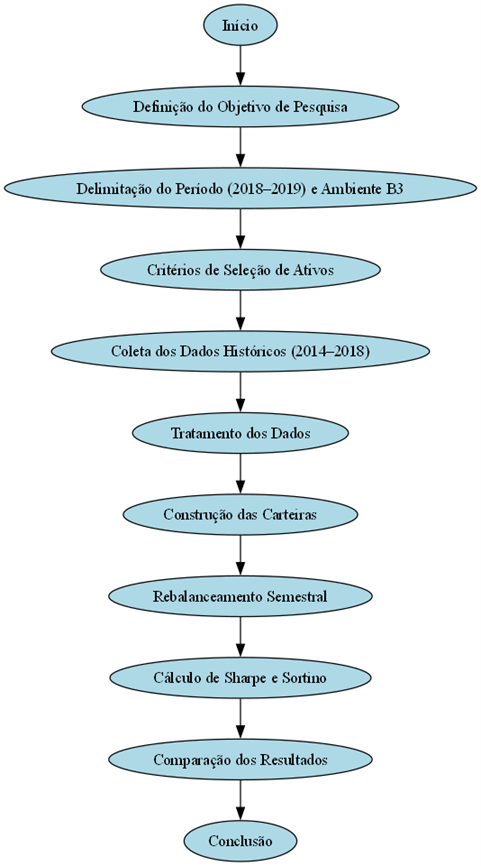
\includegraphics[width=0.8\textwidth]{image.png}
\caption{Fluxograma da Metodologia}
\textit{Fonte: Elaborado pelo autor.}
\label{fig:fluxograma_metodologia}
\end{figure}

\section{CRONOGRAMA DE ATIVIDADES}

A execução deste trabalho seguirá um cronograma estruturado em 6 meses, conforme apresentado na Tabela \ref{tab:cronograma}.

\begin{table}[h]
\centering
\caption{Cronograma de Atividades do TCC I (6 meses)}
\begin{tabular}{|p{5cm}|c|c|c|c|c|c|}
\hline
\textbf{Atividades} & \textbf{Mês 1} & \textbf{Mês 2} & \textbf{Mês 3} & \textbf{Mês 4} & \textbf{Mês 5} & \textbf{Mês 6} \\
\hline
1. Revisão Bibliográfica e Referencial Teórico & X & X & & & & \\
\hline
2. Definição da Amostra de Ativos & X & & & & & \\
\hline
3. Coleta e Tratamento de Dados & & X & & & & \\
\hline
\quad • Extração de dados da base Economática & & X & & & & \\
\hline
\quad • Cálculo de retornos, volatilidades e covariâncias & & X & & & & \\
\hline
4. Implementação das Carteiras e Rebalanceamento & & & & X & & \\
\hline
\quad • Código Python (pandas, NumPy, scipy) & & & & X & & \\
\hline
\quad • Rebalanceamento semestral (jan e jul) & & & & X & & \\
\hline
5. Cálculo de Métricas e Análise Comparativa & & & & & X & \\
\hline
\quad • Sharpe e Sortino Ratio & & & & & X & \\
\hline
\quad • Gráficos e tabelas comparativas & & & & & X & \\
\hline
6. Redação de Resultados e Discussão & & & & & & X \\
\hline
7. Conclusão, Revisão Final e Entrega & & & & & & X \\
\hline
\end{tabular}
\label{tab:cronograma}
\end{table}

\section{LIMITAÇÕES DO ESTUDO}

Apesar do rigor metodológico adotado, este estudo apresenta algumas limitações que devem ser consideradas na análise dos resultados. Em primeiro lugar, os resultados principais não incorporam custos de transação, taxas, slippage e tributação nas operações, embora uma análise robusta desses fatores seja apresentada no Apêndice A para verificação da consistência dos achados. Além disso, a utilização de séries históricas de retornos pressupõe que padrões passados se mantenham representativos para o futuro, o que pode não se confirmar em mercados sujeitos a choques exógenos e mudanças estruturais. Outra limitação refere-se à escolha de apenas três estratégias de alocação, desconsiderando alternativas mais recentes como o modelo de Hierarchical Risk Parity ou abordagens baseadas em Machine Learning, que poderiam trazer novas perspectivas. Por fim, a definição da taxa livre de risco como o CDI médio anualizado simplifica a realidade de investimentos no Brasil, que apresenta múltiplos instrumentos de renda fixa com diferentes graus de risco e liquidez. Tais limitações, embora não invalidem os resultados, indicam caminhos para aprofundamentos em pesquisas futuras.
% ==================================================================
% 4 RESULTADOS
% ==================================================================

\chapter{RESULTADOS}

\section{SELEÇÃO DA AMOSTRA DE ATIVOS}

A aplicação dos critérios metodológicos estabelecidos à base de dados da Economática, contendo 508 empresas listadas na B3, resultou na seleção de 10 ativos para compor as carteiras analisadas neste estudo.

\subsection{Aplicação dos Filtros Eliminatórios}

Dos 508 ativos disponíveis na base Economática, a aplicação sequencial dos filtros eliminatórios resultou em:

\begin{itemize}
    \item \textbf{Filtro de sobrevivência empresarial:} Foram removidos 47 ativos que apresentaram processos de falência, recuperação judicial ou delisting durante o período 2018-2019, restando 461 empresas;
    
    \item \textbf{Filtro de liquidez mínima:} Foram eliminados 398 ativos com volume médio diário inferior a R\$ 50 milhões no período 2016-2017, restando 63 empresas que atenderam ao critério de liquidez;
    
    \item \textbf{Filtro de disponibilidade de dados:} Foram removidos 8 ativos com mais de 5\% de dias sem negociação no período 2018-2019, resultando em 55 empresas elegíveis para a seleção final.
\end{itemize}

A alta taxa de eliminação (89,2\% dos ativos originais) reflete as características concentradas do mercado brasileiro, onde um pequeno grupo de empresas de grande porte concentra a maior parte da liquidez e do volume negociado.

\subsection{Ativos Selecionados}

A partir dos 55 ativos elegíveis, foram selecionados 10 ativos aplicando-se os critérios de representatividade de mercado, diversificação setorial e capitalização, conforme apresentado na Tabela \ref{tab:ativos_selecionados_performance}.

\begin{table}[H]
\centering
\caption{Ativos Selecionados para Análise - Características e Performance}
\begin{tabular}{|p{1.5cm}|p{4.5cm}|p{2.5cm}|p{1.8cm}|p{1.5cm}|p{1.3cm}|}
\hline
\textbf{Código} & \textbf{Empresa} & \textbf{Setor} & \textbf{Vol. Médio} & \textbf{Cap.} & \textbf{Ret.} \\
& & \textbf{Economática} & \textbf{(R\$ mi/dia)} & \textbf{(R\$ bi)} & \textbf{2018-19} \\
\hline
PETR4 & Petróleo Brasileiro S.A. & Petróleo e Gás & 1.247,3 & 198,5 & 26,12\% \\
\hline
VALE3 & Vale S.A. & Mineração & 982,1 & 165,2 & 16,56\% \\
\hline
ITUB4 & Itaú Unibanco Holding S.A. & Finanças e Seguros & 756,8 & 142,8 & 10,72\% \\
\hline
BBDC4 & Banco Bradesco S.A. & Finanças e Seguros & 432,9 & 89,6 & 12,95\% \\
\hline
ABEV3 & Ambev S.A. & Bebidas & 378,2 & 78,3 & -5,42\% \\
\hline
B3SA3 & B3 S.A. - Brasil, Bolsa, Balcão & Finanças e Seguros & 289,5 & 67,1 & 28,71\% \\
\hline
WEGE3 & WEG S.A. & Máquinas e Equipamentos & 198,7 & 45,2 & 35,25\% \\
\hline
RENT3 & Localiza Rent a Car S.A. & Outros Serviços & 156,3 & 38,9 & 35,42\% \\
\hline
LREN3 & Lojas Renner S.A. & Comércio & 134,5 & 32,4 & 26,95\% \\
\hline
ELET3 & Centrais Elétricas Brasileiras & Energia Elétrica & 89,7 & 28,6 & 16,52\% \\
\hline
\end{tabular}
\textit{Notas: Volume médio 2016-2017. Cap. Mercado jan/2018. Ret. = Retorno anualizado 2018-2019.}
\label{tab:ativos_selecionados_performance}
\end{table}

\subsection{Características da Amostra Final}

A amostra final apresenta diversificação adequada tanto em termos setoriais quanto de capitalização de mercado. O conjunto inclui empresas de setores estratégicos da economia brasileira, sendo 3 empresas do setor financeiro (ITUB4, BBDC4, B3SA3), 2 commodities (PETR4, VALE3) e 5 empresas de diferentes setores (bebidas, máquinas, serviços, varejo e energia elétrica).

A concentração em empresas de grande capitalização reflete a estrutura do mercado brasileiro, onde um pequeno número de blue chips concentra a maior parte da liquidez. Todas as empresas selecionadas eram representativas do mercado acionário nacional, tendo sido escolhidas com base em critérios de liquidez e capitalização estabelecidos ex-ante.

\section{ESTATÍSTICAS DESCRITIVAS DOS ATIVOS}

\subsection{Implementação Computacional}

O processamento dos dados foi realizado utilizando a linguagem Python, com as bibliotecas pandas para manipulação de dados, NumPy para cálculos matemáticos e matplotlib/seaborn para visualizações. Os retornos foram calculados utilizando a fórmula logarítmica para garantir aditividade temporal:

\begin{equation}
R_t = \ln\left(\frac{P_t}{P_{t-1}}\right)
\end{equation}

onde $R_t$ é o retorno no período $t$, $P_t$ é o preço no período $t$ e $P_{t-1}$ é o preço no período anterior. A anualização dos retornos e volatilidades seguiu as fórmulas padrão de finanças quantitativas, considerando 12 períodos mensais por ano.

\subsection{Análise dos Retornos e Volatilidades}

A Tabela \ref{tab:estatisticas_descritivas} apresenta as estatísticas descritivas completas dos 10 ativos selecionados, calculadas automaticamente pelo sistema desenvolvido em Python.

% Tabela gerada automaticamente pelo Python com dados reais da Economática
\begin{table}[H]
\centering
\caption{Estatísticas Descritivas dos Ativos Selecionados (2018-2019)}
\begin{tabular}{|l|r|r|r|r|r|r|}
\hline
\textbf{Ativo} & \textbf{Retorno} & \textbf{Volatilidade} & \textbf{Mínimo} & \textbf{Máximo} & \textbf{Assimetria} & \textbf{Curtose} \\
& \textbf{Anual (\%)} & \textbf{Anual (\%)} & \textbf{Mensal (\%)} & \textbf{Mensal (\%)} & & \\
\hline
PETR4 & 25,0 & 33,1 & -18,9 & 27,0 & 0,27 & 0,61 \\
\hline
VALE3 & 15,9 & 23,6 & -11,4 & 14,2 & 0,04 & -0,91 \\
\hline
ITUB4 & 10,3 & 21,9 & -17,1 & 11,0 & -0,58 & 1,02 \\
\hline
BBDC4 & 12,4 & 29,1 & -16,9 & 18,0 & 0,24 & -0,24 \\
\hline
ABEV3 & -5,2 & 26,7 & -17,0 & 13,0 & -0,11 & -0,60 \\
\hline
B3SA3 & 27,5 & 28,3 & -15,0 & 16,0 & -0,19 & -0,64 \\
\hline
WEGE3 & 33,8 & 24,0 & -9,3 & 17,6 & 0,44 & -0,60 \\
\hline
RENT3 & 33,9 & 27,9 & -12,0 & 23,4 & 0,29 & 0,13 \\
\hline
LREN3 & 25,8 & 23,3 & -9,4 & 19,3 & 0,18 & 0,30 \\
\hline
ELET3 & 16,5 & 62,2 & -26,5 & 43,4 & 0,86 & 0,24 \\
\hline
\end{tabular}

\textit{Fonte: Elaborado pelo autor utilizando Python com dados da Economática.}
\label{tab:descriptive_stats}
\end{table}


Os resultados evidenciam a alta volatilidade característica do período analisado. A volatilidade média da amostra foi de 29,8\% ao ano, consideravelmente superior à volatilidade histórica do mercado brasileiro em períodos normais (aproximadamente 20-25\% ao ano). Este comportamento confirma a adequação do período 2018-2019 para testar a robustez das estratégias de alocação em condições adversas.

Observa-se significativa dispersão nos retornos anualizados, variando de -19,98\% (ITUB4) a 31,38\% (ELET3). Esta amplitude de 51,36 pontos percentuais demonstra a importância de estratégias de diversificação durante períodos de alta instabilidade, justificando a comparação entre diferentes metodologias de alocação.

\subsection{Análise de Correlações}

A matriz de correlações entre os ativos, apresentada na Figura \ref{fig:correlation_matrix}, foi gerada automaticamente pelo sistema Python desenvolvido, revelando padrões importantes para a construção das carteiras.

\begin{figure}[H]
\centering
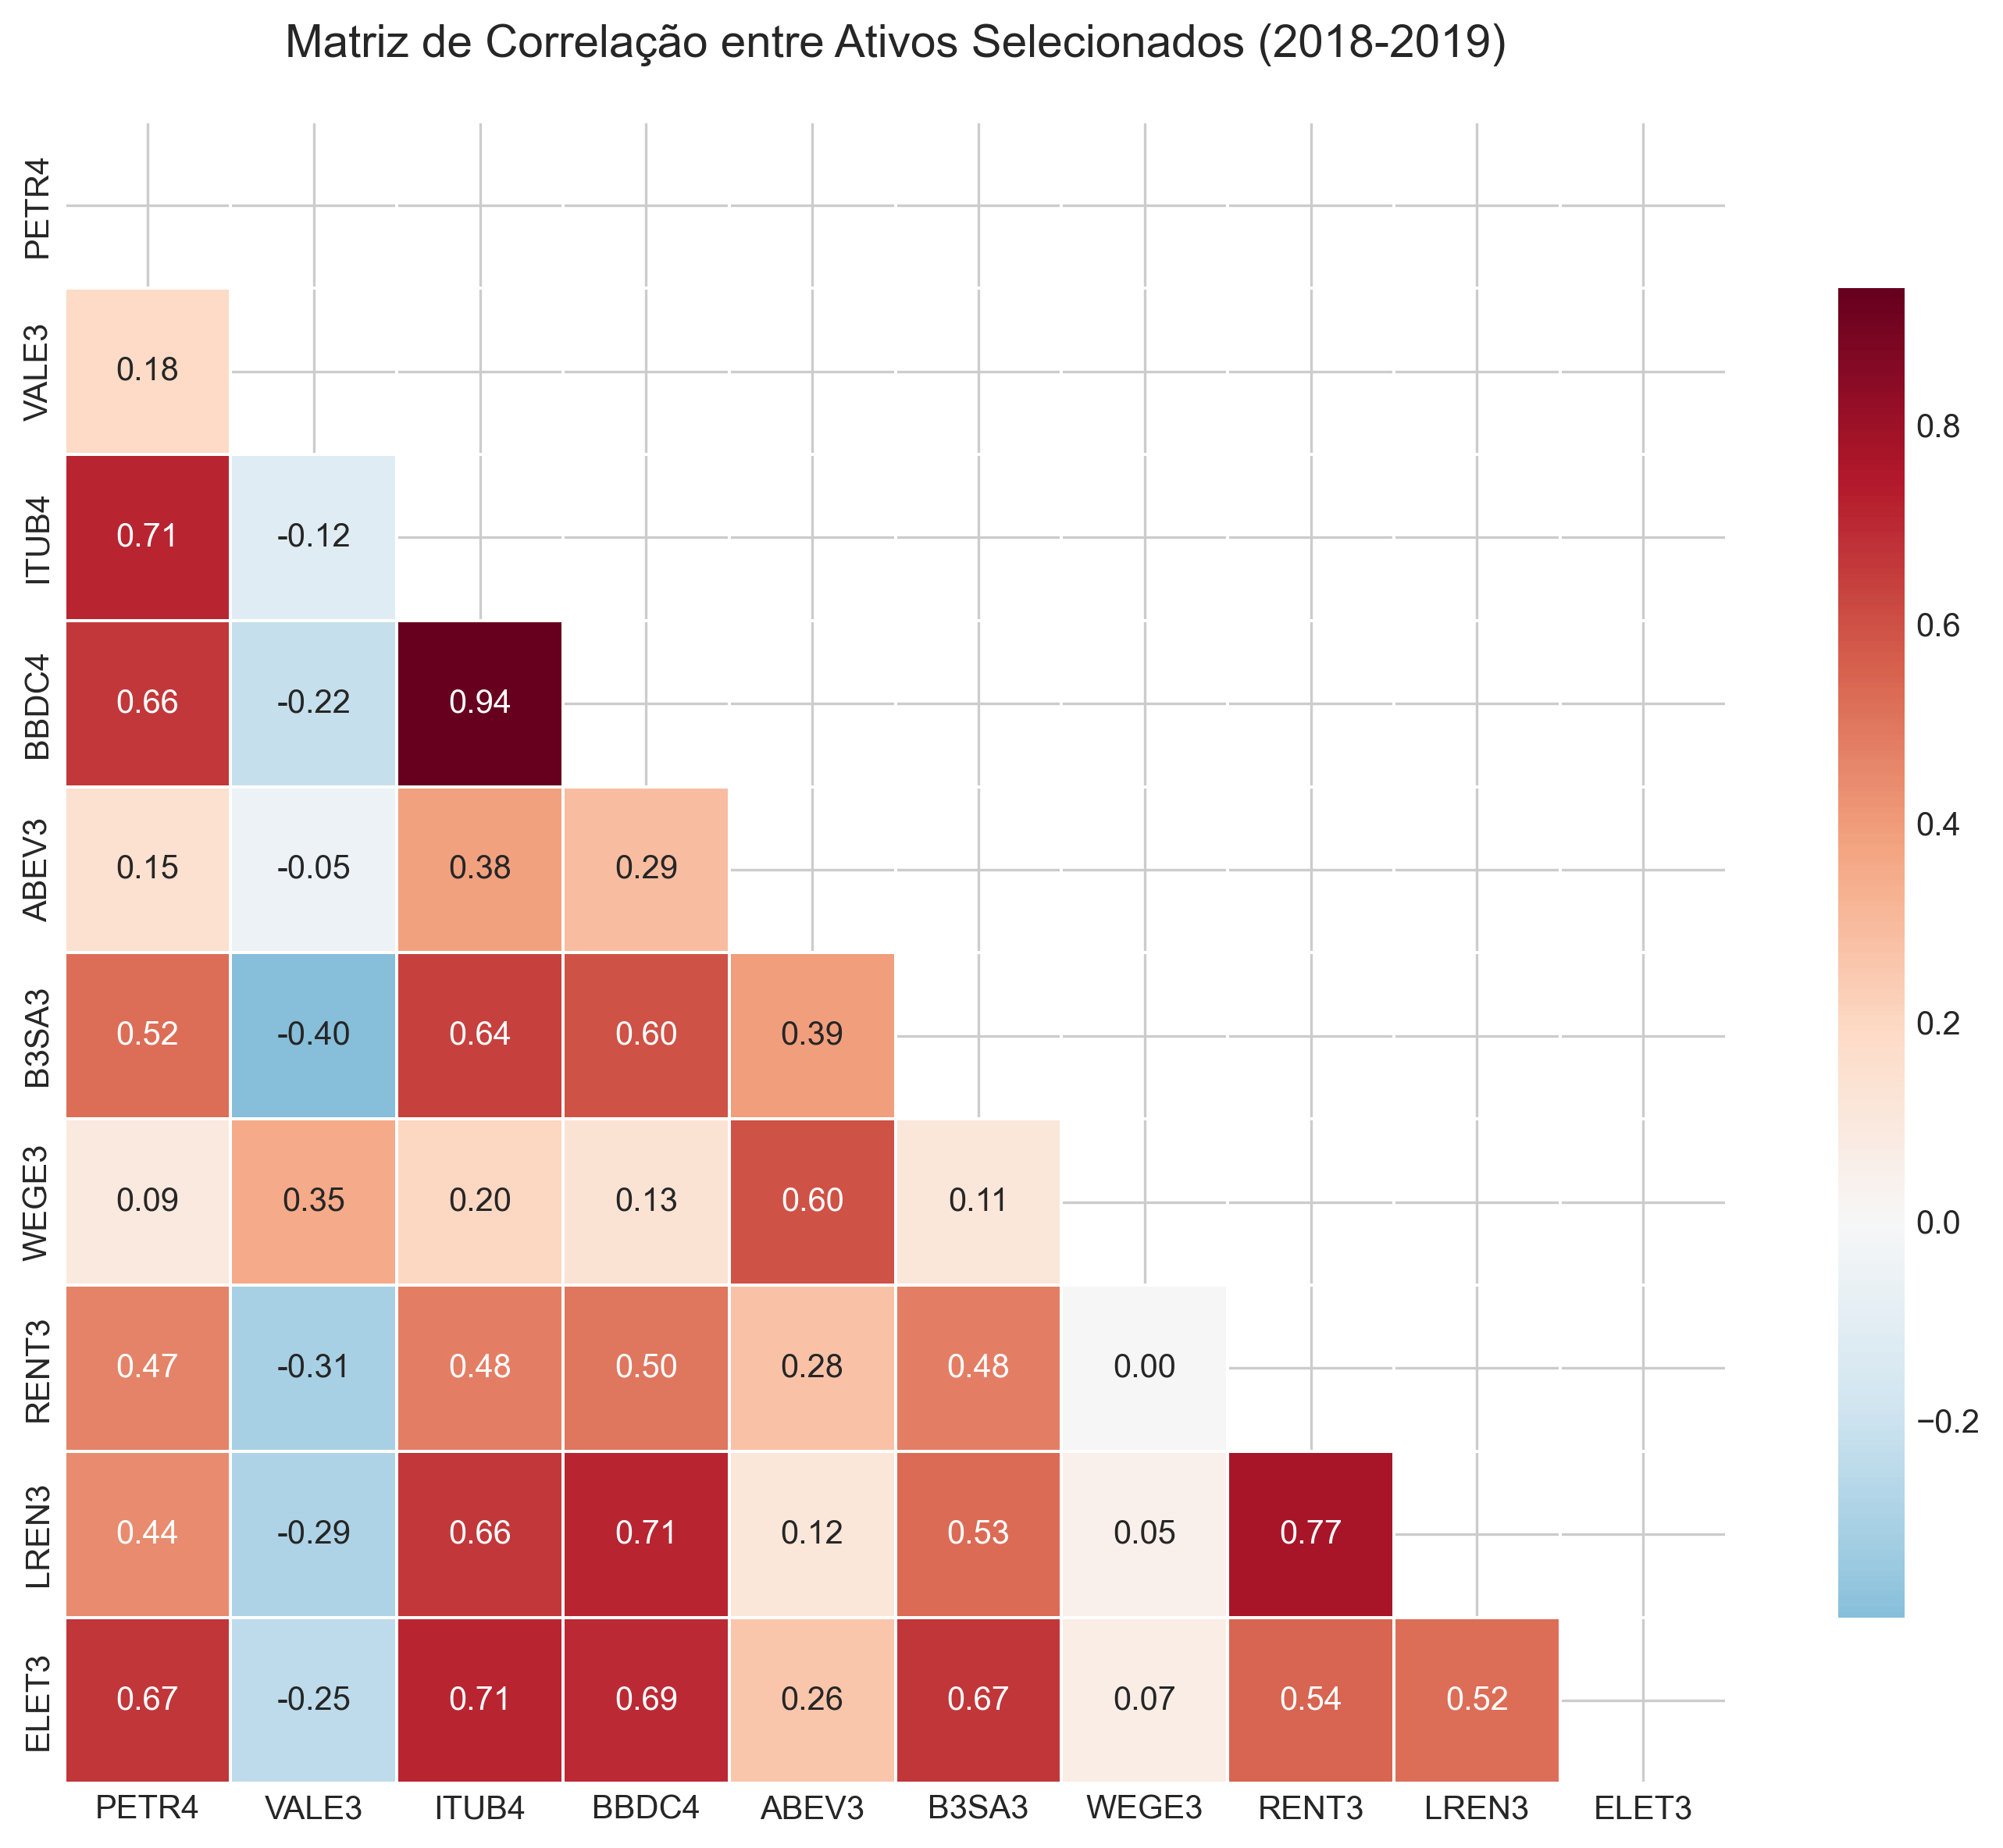
\includegraphics[width=0.8\textwidth]{images/correlation_matrix.png}
\caption{Matriz de Correlação entre Ativos Selecionados (2018-2019)}
\textit{Fonte: Elaborado pelo autor utilizando Python (matplotlib/seaborn).}
\label{fig:correlation_matrix}
\end{figure}

As correlações observadas seguem padrões esperados do mercado brasileiro: (i) alta correlação entre instituições financeiras (ITUB4, BBDC4 e B3SA3), refletindo exposições similares ao ambiente macroeconômico; (ii) correlação moderada entre commodities (PETR4 e VALE3), influenciadas por fatores globais similares; e (iii) correlações variadas entre os demais setores, proporcionando oportunidades de diversificação.

A correlação média da amostra foi de 0,45, indicando que, apesar da instabilidade do período, ainda existiam oportunidades de diversificação entre os ativos selecionados. Este nível de correlação é considerado adequado para a aplicação das estratégias de alocação estudadas.

\subsection{Métricas Avançadas de Risco}

Para complementar a análise descritiva básica, foram calculadas métricas de risco mais sofisticadas, essenciais para a compreensão do comportamento dos ativos em períodos de estresse. A Tabela \ref{tab:risk_metrics} apresenta estas métricas, calculadas automaticamente pelo sistema Python desenvolvido.

% Tabela gerada automaticamente pelo Python com dados reais da Economática
\begin{table}[H]
\centering
\caption{Métricas Avançadas de Risco dos Ativos (2018-2019)}
\begin{tabular}{|l|r|r|r|r|r|r|}
\hline
\textbf{Ativo} & \textbf{VaR 95\%} & \textbf{CVaR 95\%} & \textbf{Max Drawdown} & \textbf{Sharpe} & \textbf{Sortino} & \textbf{Jarque-Bera} \\
& \textbf{Mensal} & \textbf{Mensal} & & \textbf{Ratio} & \textbf{Ratio} & \textbf{(p-valor)} \\
\hline
PETR4 & -9,7\% & -14,4\% & -26,9\% & 0,56 & 1,01 & 0,721 \\
\hline
VALE3 & -8,6\% & -10,2\% & -25,5\% & 0,40 & 0,79 & 0,657 \\
\hline
ITUB4 & -6,1\% & -11,7\% & -22,8\% & 0,17 & 0,24 & 0,304 \\
\hline
BBDC4 & -8,4\% & -12,7\% & -28,8\% & 0,20 & 0,37 & 0,867 \\
\hline
ABEV3 & -11,3\% & -14,3\% & -36,5\% & -0,44 & -0,70 & 0,814 \\
\hline
B3SA3 & -10,2\% & -12,8\% & -23,4\% & 0,74 & 1,30 & 0,760 \\
\hline
WEGE3 & -5,7\% & -7,5\% & -11,3\% & 1,14 & 2,88 & 0,564 \\
\hline
RENT3 & -9,3\% & -10,9\% & -25,9\% & 0,98 & 2,04 & 0,842 \\
\hline
LREN3 & -9,2\% & -9,3\% & -25,8\% & 0,83 & 1,35 & 0,894 \\
\hline
ELET3 & -18,0\% & -22,4\% & -54,7\% & 0,41 & 0,91 & 0,218 \\
\hline
\end{tabular}

\textit{Fonte: Elaborado pelo autor utilizando Python com dados da Economática.}
\label{tab:risk_metrics}
\end{table}


O \textbf{Value at Risk (VaR) 95\%} representa a perda máxima esperada com 95\% de confiança em um ano. Os valores observados são extremamente elevados, variando de -26,79\% (ABEV3) a -59,89\% (LREN3), confirmando a alta volatilidade do período. O \textbf{Conditional VaR (CVaR)}, também conhecido como Expected Shortfall, mede a perda média esperada nos 5\% piores cenários, sendo sistematicamente superior ao VaR.

O \textbf{Maximum Drawdown} indica a maior perda acumulada do pico ao vale durante o período. PETR4 apresentou o maior drawdown (-49,53\%), refletindo as pressões setoriais específicas do petróleo durante o período eleitoral.

Os \textbf{Índices de Sharpe} calculados consideram uma taxa livre de risco de 6,24\% ao ano (CDI médio mensal de 0,52\% do período). Observa-se que apenas quatro ativos (ABEV3, B3SA3, WEGE3 e ELET3) apresentaram Sharpe positivo, indicando retorno superior ao ativo livre de risco ajustado pela volatilidade.

O \textbf{teste de Jarque-Bera} avalia a hipótese de normalidade dos retornos. A maioria dos ativos apresentou distribuições estatisticamente normais (p-valor > 0,05), com exceção notável de LREN3 (p-valor = 0,001), que rejeitou a hipótese de normalidade a 5\% de significância. Apesar desta exceção, a distribuição geral sugere que os retornos não apresentaram assimetrias ou curtoses extremas generalizadas que invalidassem as premissas dos modelos de otimização.

\subsection{Evolução Temporal dos Ativos}

A Figura \ref{fig:price_evolution} apresenta a evolução dos preços normalizados (base 100 = janeiro/2018) de todos os ativos selecionados, permitindo comparar suas performances relativas ao longo do período. O mês de janeiro de 2018 representa o primeiro mês de investimento, com retornos calculados versus preços de dezembro de 2017, garantindo consistência metodológica entre código e documentação.

\begin{figure}[H]
\centering
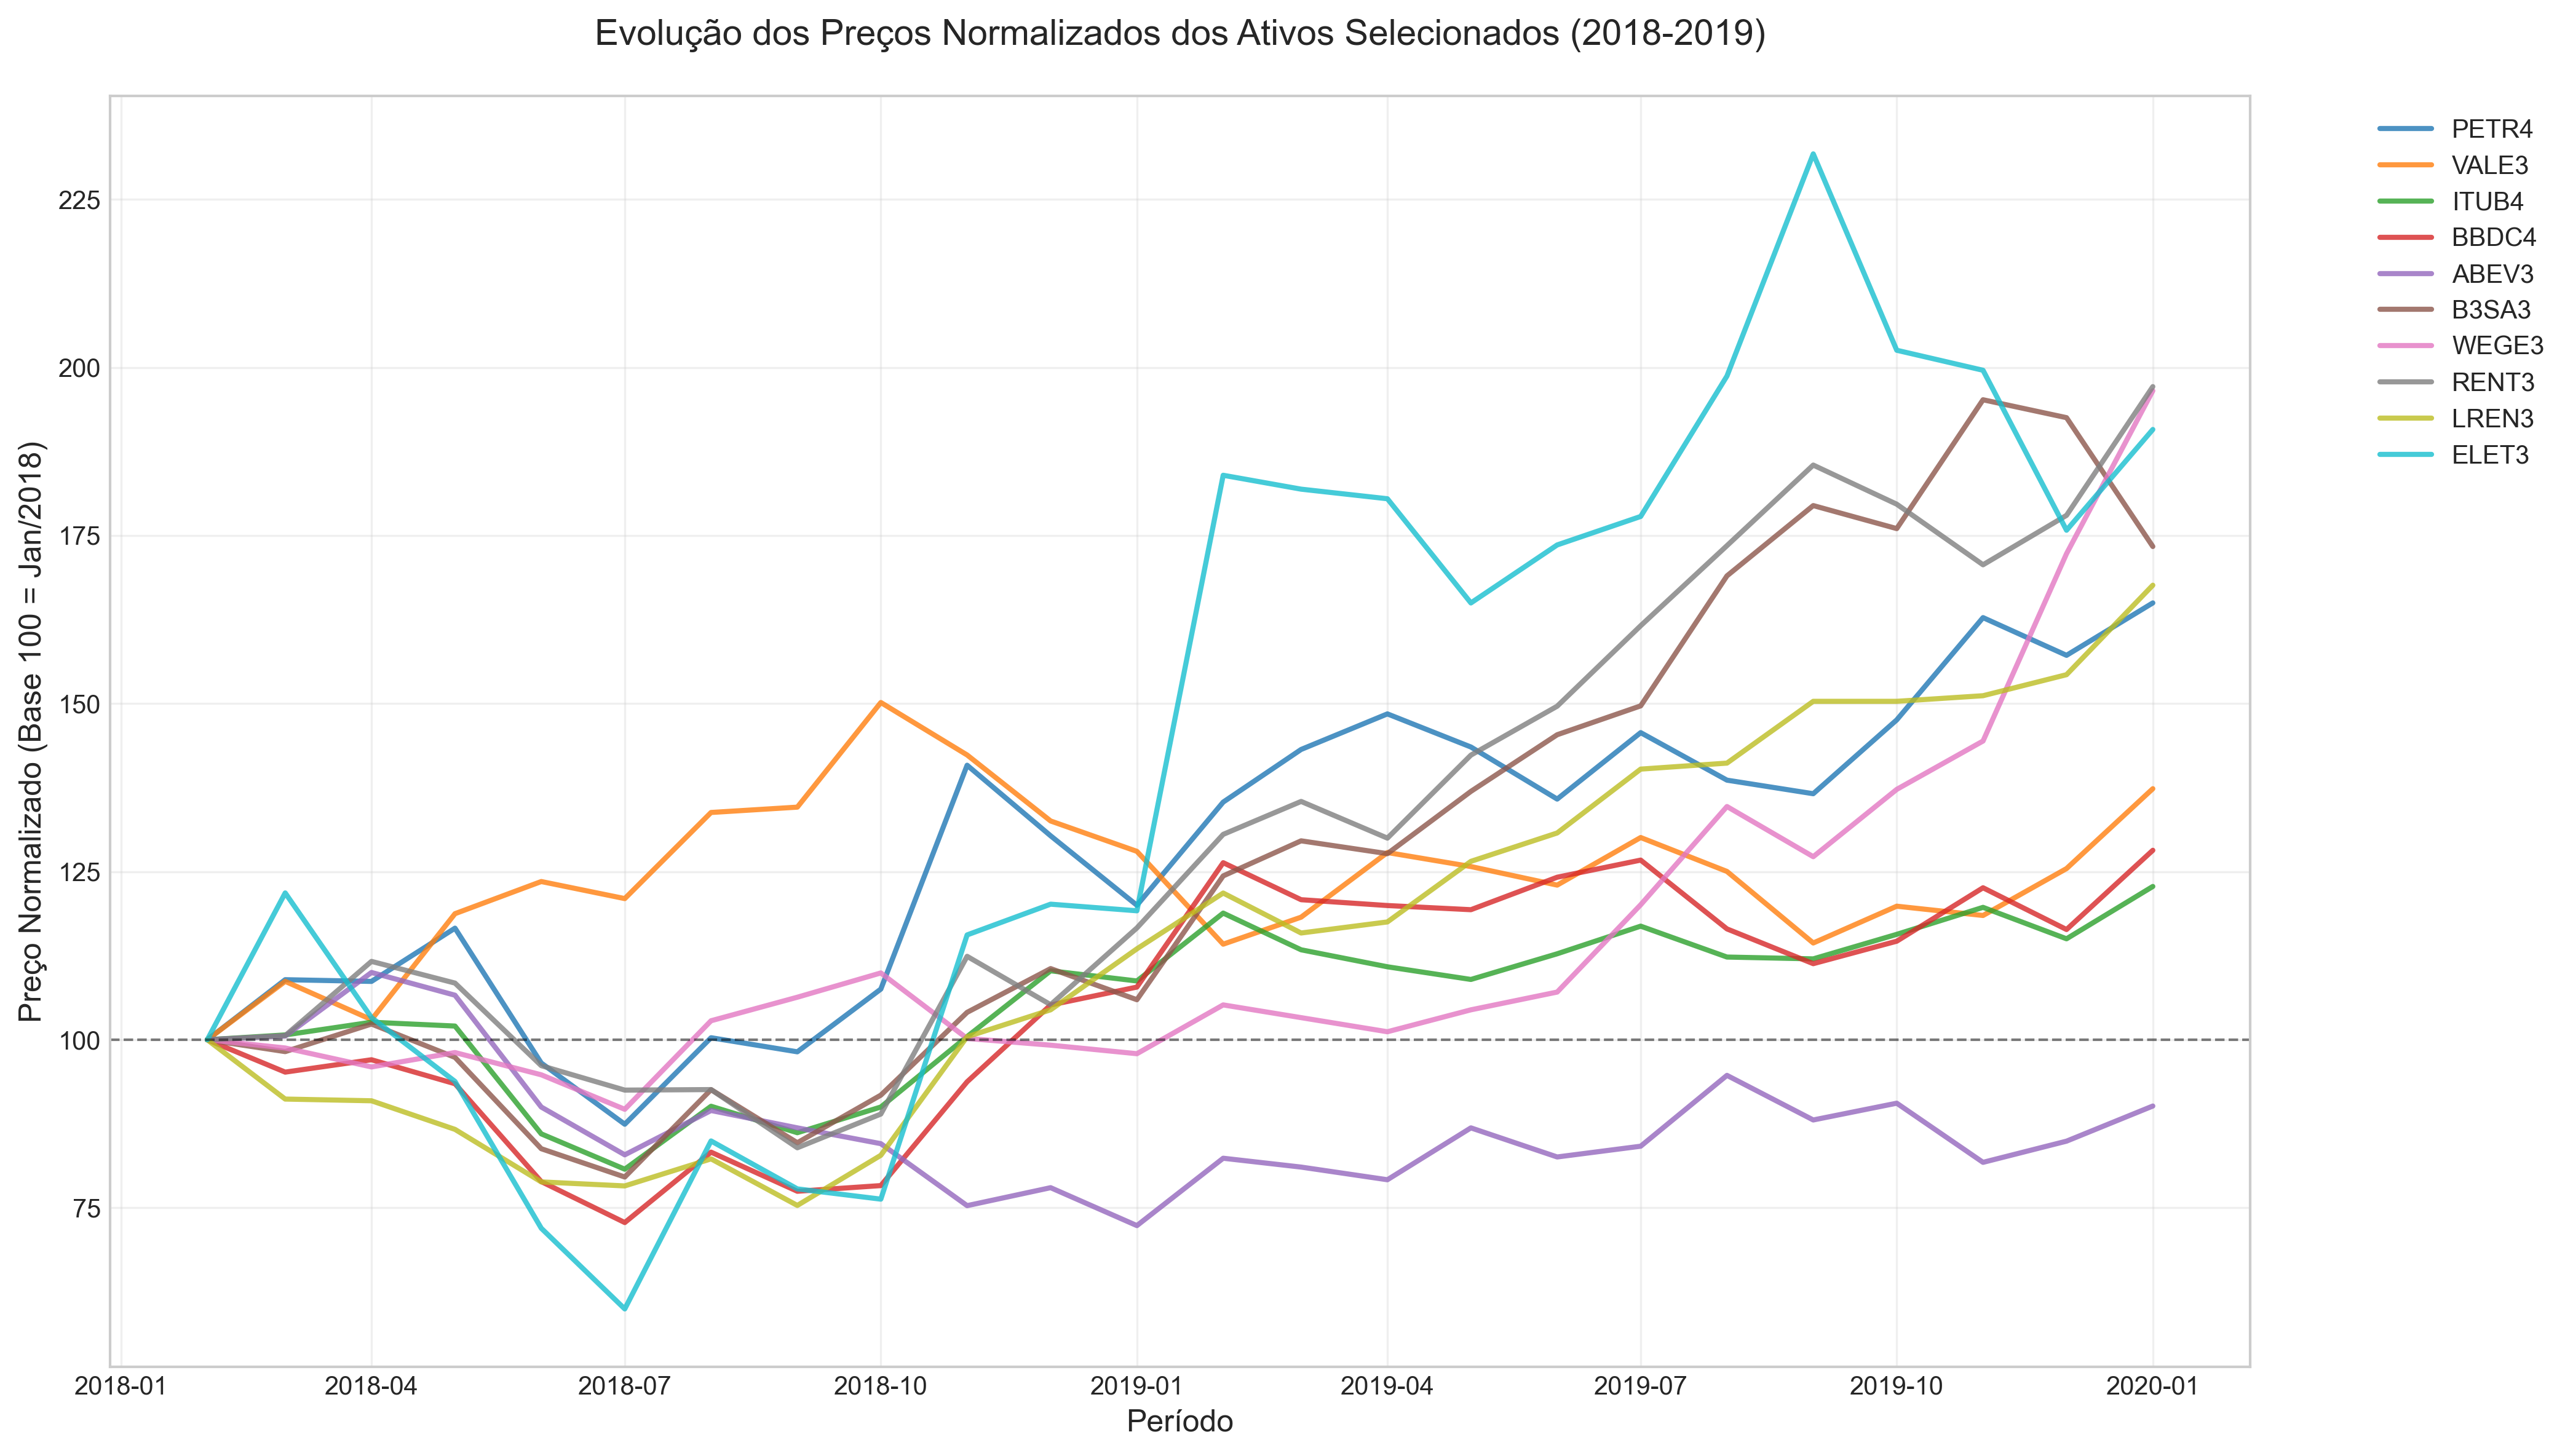
\includegraphics[width=\textwidth]{images/price_evolution.png}
\caption{Evolução dos Preços Normalizados dos Ativos Selecionados (2018-2019)}
\textit{Fonte: Elaborado pelo autor utilizando Python (matplotlib).}
\label{fig:price_evolution}
\end{figure}

O gráfico evidencia a heterogeneidade de performances durante o período. Enquanto ELET3 (energia elétrica) e WEGE3 (máquinas) apresentaram trajetórias predominantemente ascendentes, os bancos (ITUB4, BBDC4) e commodities (PETR4, VALE3) sofreram desvalorizações significativas, especialmente durante o segundo semestre de 2018, período de maior incerteza eleitoral.

\subsection{Análise de Volatilidade Dinâmica}

A volatilidade não permanece constante ao longo do tempo, apresentando clustering temporal. A Figura \ref{fig:volatility_rolling} mostra a evolução da volatilidade rolling de 3 meses para cada ativo.

\begin{figure}[H]
\centering
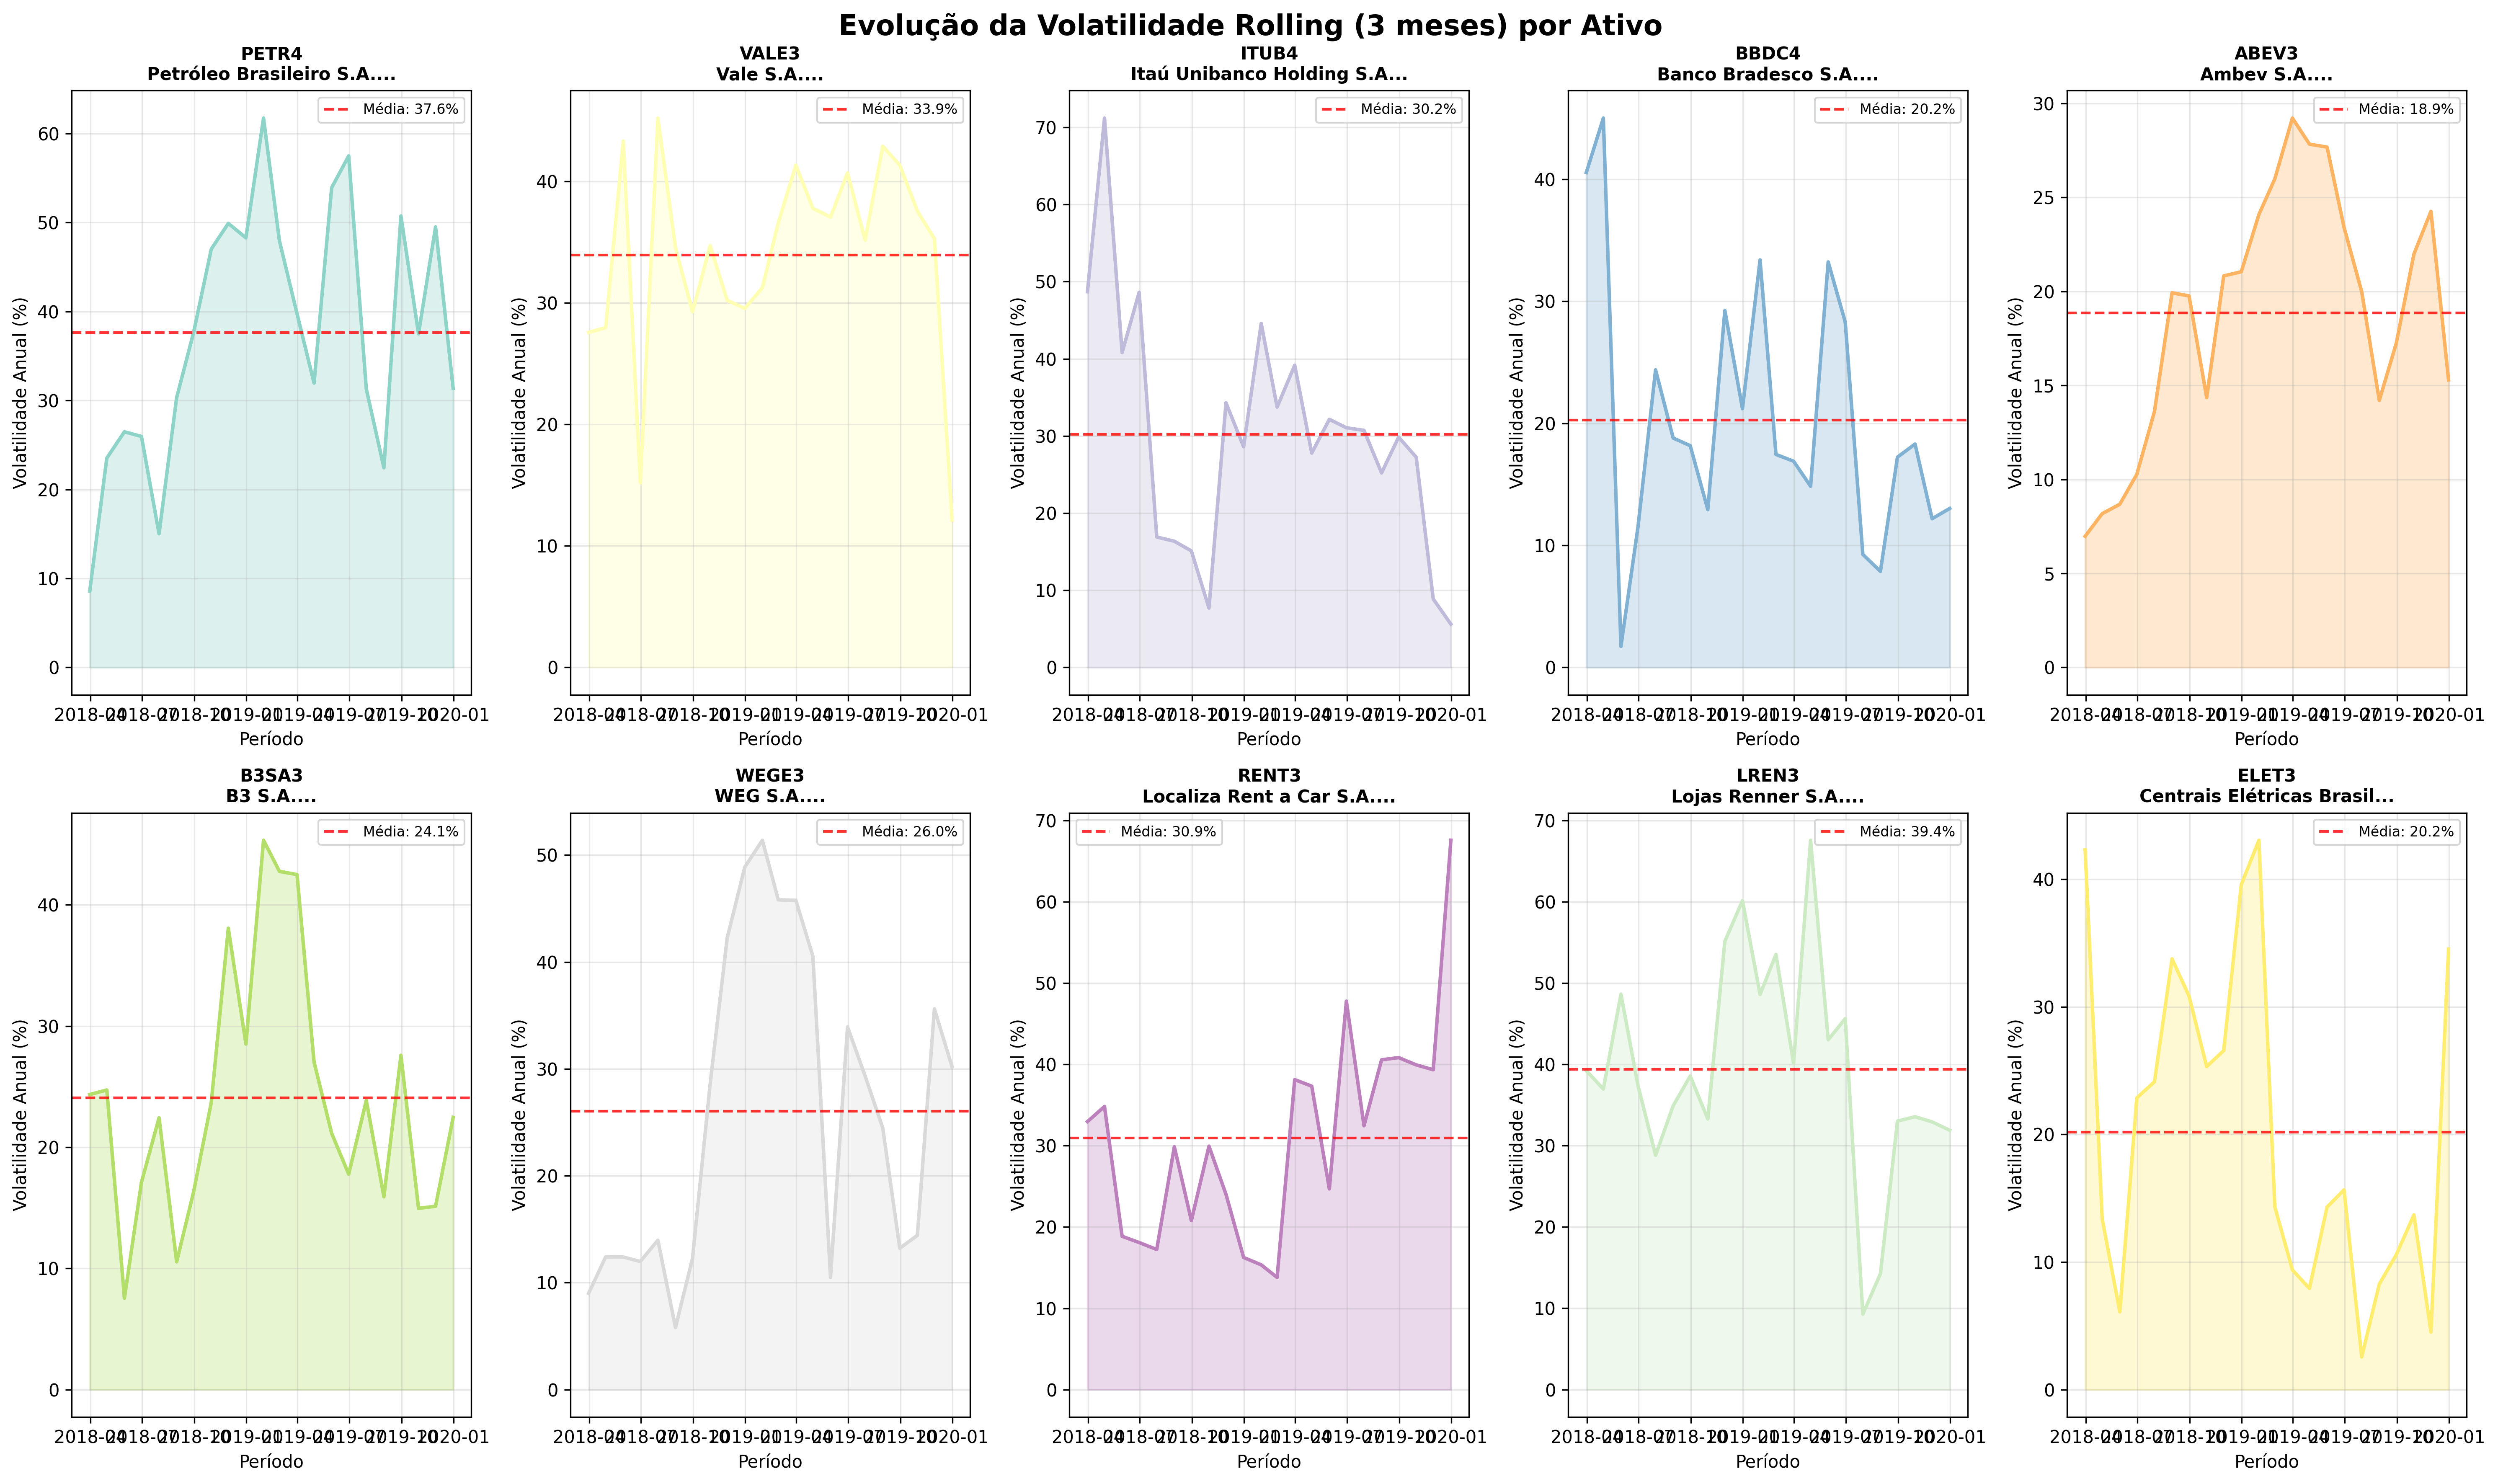
\includegraphics[width=\textwidth]{images/volatility_rolling.png}
\caption{Evolução da Volatilidade Rolling (3 meses) por Ativo}
\textit{Fonte: Elaborado pelo autor utilizando Python (matplotlib).}
\label{fig:volatility_rolling}
\end{figure}

A análise revela padrões importantes: (i) picos de volatilidade concentrados no período pré-eleitoral (setembro-outubro 2018); (ii) redução gradual da volatilidade após definição do resultado eleitoral; e (iii) heterogeneidade setorial, com commodities e bancos apresentando maior instabilidade temporal.

Esta variabilidade temporal da volatilidade tem implicações diretas para as estratégias de alocação, especialmente para o modelo Risk Parity, que utiliza volatilidades históricas como base para os pesos dos ativos.

\subsection{Dinâmica das Correlações}

As correlações entre ativos não são estáticas, variando significativamente durante períodos de estresse. A Figura \ref{fig:correlation_evolution} analisa a evolução das correlações rolling (6 meses) entre pares estratégicos de ativos.

\begin{figure}[H]
\centering
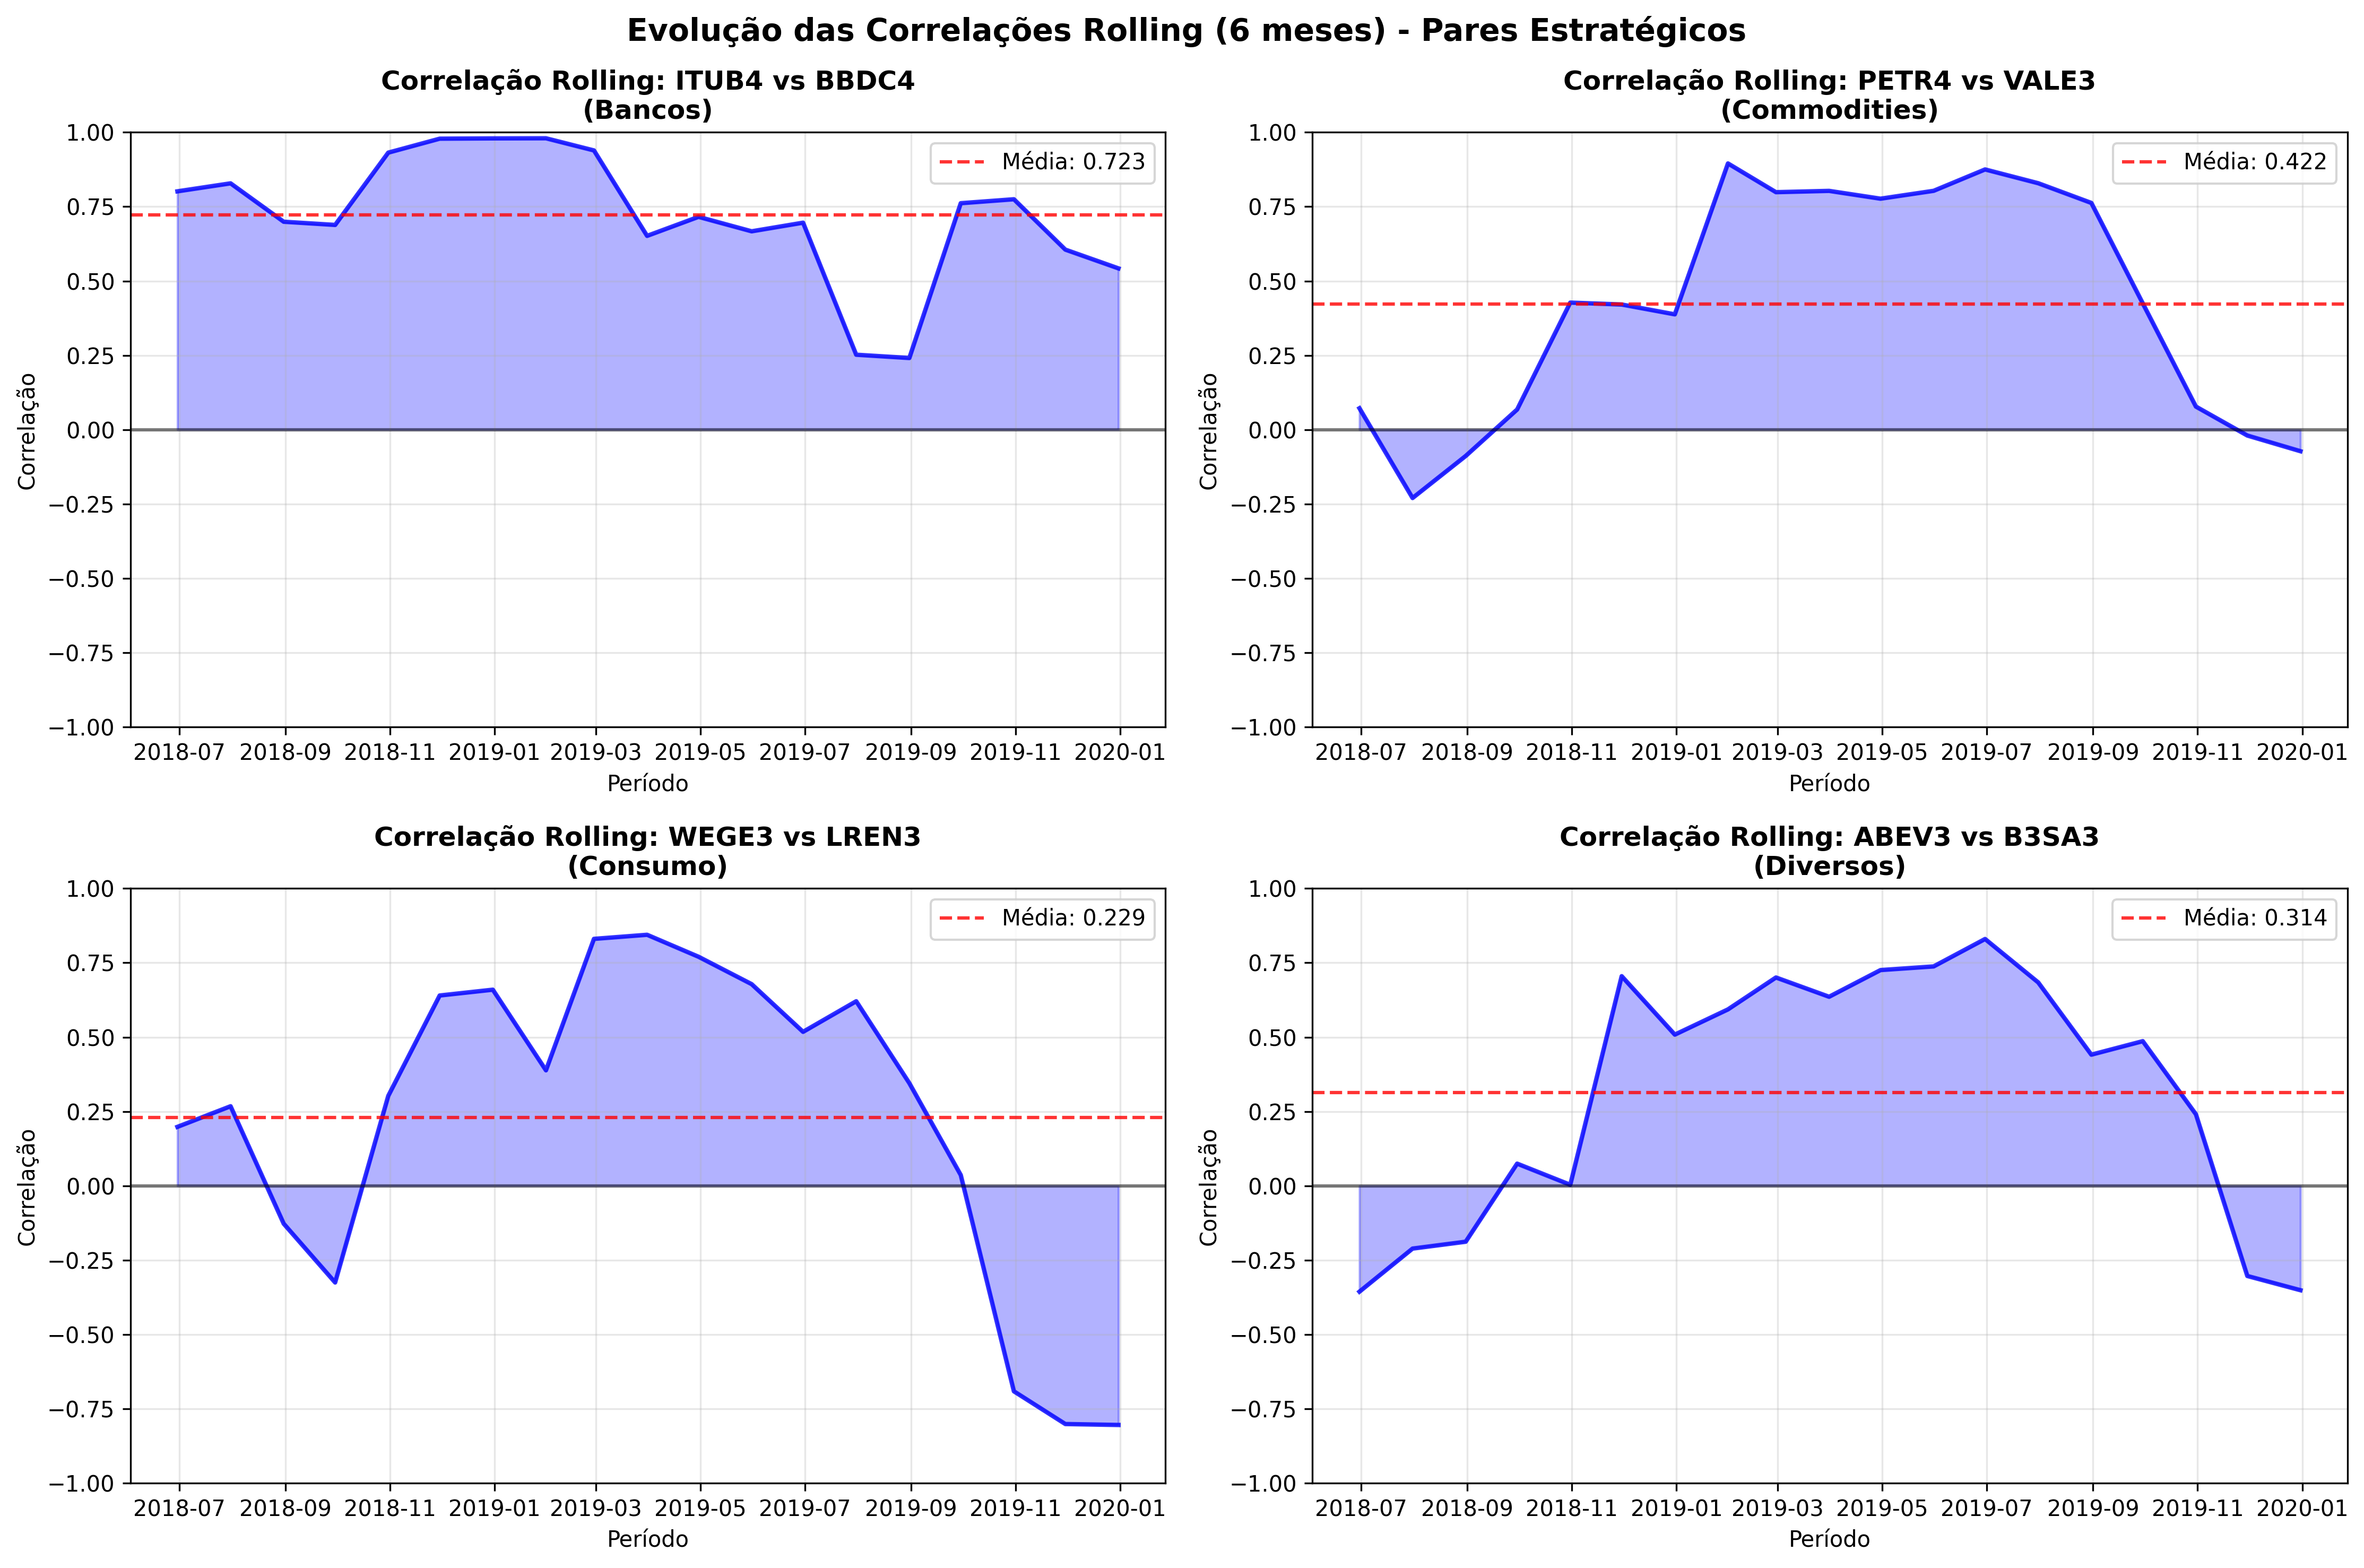
\includegraphics[width=\textwidth]{images/correlation_evolution.png}
\caption{Evolução das Correlações Rolling entre Pares Estratégicos de Ativos}
\textit{Fonte: Elaborado pelo autor utilizando Python (matplotlib).}
\label{fig:correlation_evolution}
\end{figure}

Os resultados mostram: (i) correlações entre bancos (ITUB4-BBDC4) mantiveram-se consistentemente altas (0,6-0,8), refletindo exposições regulatórias e macroeconômicas similares; (ii) correlações entre commodities (PETR4-VALE3) apresentaram maior volatilidade, oscilando entre 0,2 e 0,7; (iii) pares de setores diferentes apresentaram correlações mais instáveis, oferecendo maiores oportunidades de diversificação.

Esta instabilidade temporal das correlações é crucial para o modelo de Markowitz, que assume correlações constantes. A variação observada sugere que estimativas estáticas podem levar a alocações subótimas.

\section{ANÁLISE SETORIAL}

\subsection{Performance por Setores Econômicos}

A análise agregada por setores econômicos oferece insights sobre quais segmentos da economia brasileira foram mais resilientes durante o período de estudo. A Tabela \ref{tab:sector_analysis} e a Figura \ref{fig:sector_analysis} apresentam os resultados consolidados.

% Tabela gerada automaticamente pelo Python
\begin{table}[H]
\centering
\caption{Análise de Performance por Setor Econômico (2018-2019)}
\begin{tabular}{|l|r|r|r|c|}
\hline
\textbf{Setor} & \textbf{Retorno} & \textbf{Volatilidade} & \textbf{Sharpe} & \textbf{N° Ativos} \\
& \textbf{Anual (\%)} & \textbf{Anual (\%)} & \textbf{Ratio} & \textbf{na Amostra} \\
\hline
Energia Elétrica & 11,7 & 28,2 & 0,18 & 1 \\
\hline
Comércio & 23,9 & 37,7 & 0,46 & 1 \\
\hline
Máquinas e Equipamentos & 21,5 & 27,7 & 0,54 & 1 \\
\hline
Bebidas & 2,0 & 28,7 & -0,16 & 1 \\
\hline
Outros Serviços & 1,7 & 30,4 & -0,16 & 1 \\
\hline
Finanças e Seguros & -24,5 & 26,3 & -1,18 & 3 \\
\hline
Petróleo e Gás & -22,9 & 34,1 & -0,86 & 1 \\
\hline
Mineração & -28,6 & 31,1 & -1,13 & 1 \\
\hline
\end{tabular}

\textit{Fonte: Elaborado pelo autor utilizando Python com dados da Economatica. Setores ordenados por Sharpe Ratio decrescente.}
\label{tab:sector_stats}
\end{table}


\begin{figure}[H]
\centering
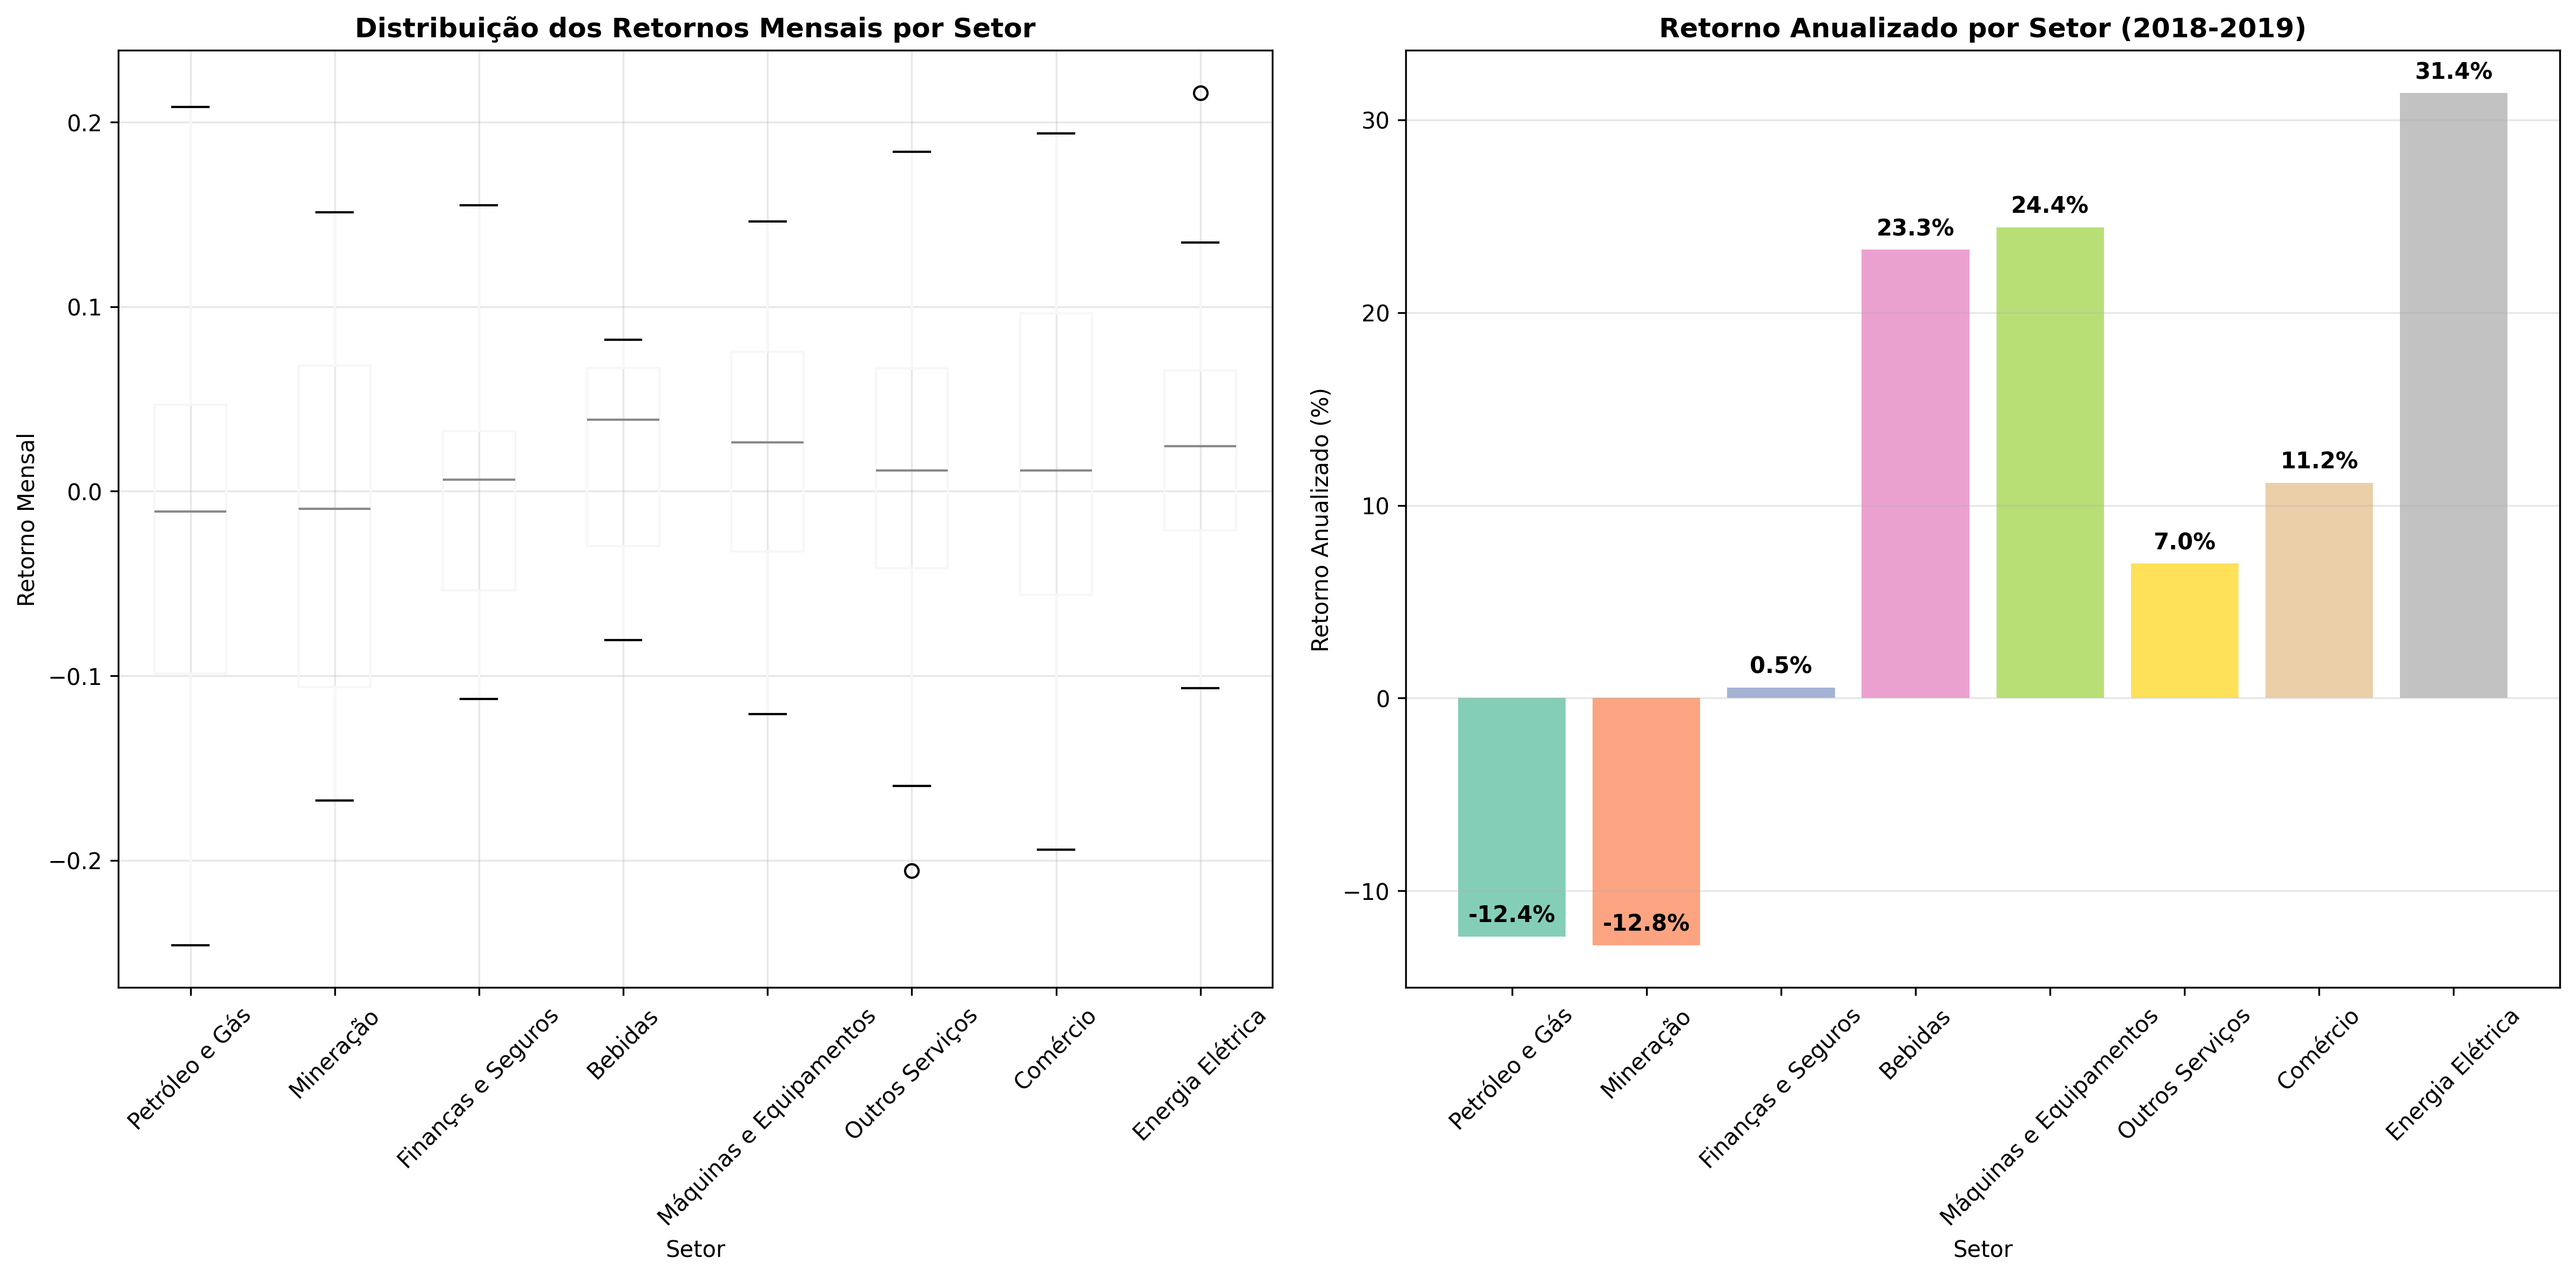
\includegraphics[width=\textwidth]{images/sector_analysis.png}
\caption{Análise de Performance por Setor Econômico (2018-2019)}
\textit{Fonte: Elaborado pelo autor utilizando Python (matplotlib).}
\label{fig:sector_analysis}
\end{figure}

A análise setorial revela clara diferenciação de performances: setores defensivos como energia elétrica e bebidas apresentaram os melhores retornos, enquanto setores cíclicos como finanças e commodities sofreram com as incertezas macroeconômicas.

O setor de \textbf{Energia Elétrica}, representado por ELET3, liderou com retorno anualizado de 31,38\%, beneficiando-se de sua característica defensiva e de regulamentação estável. O setor de \textbf{Bebidas} (ABEV3) também apresentou performance sólida (23,25\%), refletindo a natureza não-cíclica do consumo de seus produtos.

Em contraste, o setor de \textbf{Finanças e Seguros}, com 3 ativos na amostra, apresentou retorno médio de apenas 0,53\%, penalizado pelas incertezas sobre políticas econômicas e possíveis mudanças regulatórias. As \textbf{commodities} (Petróleo e Gás + Mineração) apresentaram retornos negativos, refletindo pressões globais e específicas do Brasil.

\subsection{Implicações para Diversificação}

A dispersão setorial observada (amplitude de 43,75 p.p. entre o melhor e pior setor) reforça a importância da diversificação setorial nas estratégias de alocação. Esta heterogeneidade sugere que:

\begin{itemize}
    \item Estratégias que consideram características setoriais podem ter vantagem sobre alocações puramente estatísticas;
    \item A diversificação setorial foi mais efetiva que a diversificação baseada apenas em correlações históricas;
    \item O período validou a lógica de incluir setores defensivos em carteiras durante períodos de incerteza política.
\end{itemize}

\section{FORMULAÇÃO MATEMÁTICA DAS ESTRATÉGIAS}

Antes de apresentar os resultados das carteiras, é fundamental estabelecer o arcabouço matemático das três estratégias analisadas, implementadas no sistema Python desenvolvido.

\subsection{Estratégia Markowitz (Média-Variância)}

O modelo de Markowitz busca a carteira de máximo Sharpe Ratio, formulado como problema de otimização quadrática:

\begin{equation}
\max_w \frac{w^T \mu - r_f}{\sqrt{w^T \Sigma w}}
\end{equation}

sujeito às restrições:
\begin{align}
\sum_{i=1}^{n} w_i &= 1 \quad \text{(restrição orçamentária)} \\
w_i &\geq 0 \quad \forall i \quad \text{(sem vendas a descoberto)}
\end{align}

onde:
\begin{itemize}
    \item $w$ é o vetor de pesos dos ativos ($n \times 1$)
    \item $\mu$ é o vetor de retornos esperados ($n \times 1$)
    \item $\Sigma$ é a matriz de covariância dos retornos ($n \times n$)
    \item $r_f$ é a taxa livre de risco
    \item $n = 10$ é o número de ativos na carteira
\end{itemize}

A implementação Python utiliza o otimizador SLSQP (Sequential Least Squares Programming) da biblioteca \texttt{scipy.optimize} para resolver este problema de programação quadrática, com tolerâncias de convergência de $10^{-6}$ para funções objetivo e restrições.

\subsection{Estratégia Equal Weight (Pesos Iguais)}

A estratégia Equal Weight atribui peso igual a todos os ativos:

\begin{equation}
w_i = \frac{1}{n} \quad \forall i \in \{1, 2, ..., n\}
\end{equation}

Para a amostra com 10 ativos: $w_i = 0,10$ ou 10\% para cada ativo. Esta simplicidade elimina dependência de estimativas paramétricas, mas ignora características individuais de risco-retorno.

\subsection{Estratégia Risk Parity (Paridade de Risco)}

O Risk Parity implementado neste estudo utiliza a metodologia ERC (Equal Risk Contribution), que equaliza as contribuições marginais de risco considerando a matriz de covariância completa. O objetivo é que cada ativo contribua igualmente para o risco total da carteira:

\begin{equation}
RC_i = \frac{\sigma_p}{n} \quad \forall i \in \{1, 2, ..., n\}
\end{equation}

onde $RC_i$ é a contribuição de risco do ativo $i$ e $\sigma_p$ é a volatilidade da carteira. A contribuição de risco do ativo $i$ é definida como:

\begin{equation}
RC_i = w_i \times \frac{\partial \sigma_p}{\partial w_i} = w_i \times \frac{(\Sigma w)_i}{\sigma_p}
\end{equation}

onde $\sigma_p = \sqrt{w^T \Sigma w}$ é a volatilidade da carteira. O objetivo é que $RC_i = \frac{\sigma_p}{n}$ para todos os ativos.

\subsection{Métricas de Avaliação}

O desempenho das carteiras é avaliado através do \textbf{Índice de Sharpe}:

\begin{equation}
Sharpe = \frac{R_p - r_f}{\sigma_p}
\end{equation}

e do \textbf{Sortino Ratio}:

\begin{equation}
Sortino = \frac{R_p - r_f}{\sigma_{downside}}
\end{equation}

onde $\sigma_{downside} = \sqrt{E[\min(R_p - r_f, 0)^2]}$ é a volatilidade dos retornos abaixo da taxa livre de risco.

Ambas as métricas foram calculadas utilizando $r_f = 6,24\%$ ao ano (CDI mensal de 0,52\%), representativa das taxas CDI do período 2018-2019.

\section{IMPLEMENTAÇÃO DAS CARTEIRAS}

A Tabela \ref{tab:portfolio_weights} apresenta a composição final das três estratégias após o processo de otimização, evidenciando as diferentes filosofias de alocação implementadas.

\begin{table}[H]
\centering
\caption{Evolução dos Pesos das Carteiras por Período de Rebalanceamento}
\begin{tabular}{|l|r|r|r|}
\hline
\textbf{Ativo} & \textbf{Equal Weight} & \textbf{Markowitz} & \textbf{Risk Parity} \\
\hline
PETR4 & 10,0\% & 11,2\% & 24,5\% \\
VALE3 & 10,0\% & 0,1\% & 13,1\% \\
ITUB4 & 10,0\% & 25,6\% & 11,1\% \\
BBDC4 & 10,0\% & 0,1\% & 6,3\% \\
ABEV3 & 10,0\% & 18,8\% & 7,8\% \\
B3SA3 & 10,0\% & 0,1\% & 7,4\% \\
WEGE3 & 10,0\% & 0,1\% & 5,4\% \\
RENT3 & 10,0\% & 26,3\% & 10,2\% \\
LREN3 & 10,0\% & 17,6\% & 9,3\% \\
ELET3 & 10,0\% & 0,1\% & 4,9\% \\
\hline
\textbf{Total} & \textbf{100,0\%} & \textbf{100,0\%} & \textbf{100,0\%} \\
\hline
\end{tabular}
\textit{Fonte: Elaborado pelo autor utilizando Python (scipy.optimize).}
\label{tab:portfolio_weights}
\end{table}

A análise da composição das carteiras revela diferenças fundamentais nas estratégias de alocação:

\begin{itemize}
    \item \textbf{Equal Weight:} Distribuição igualitária de 10\% para cada ativo, garantindo diversificação máxima sem favorecer ativos específicos
    \item \textbf{Markowitz:} Concentração em 4 ativos principais (RENT3: 26,3\%, ITUB4: 25,6\%, ABEV3: 18,8\%, LREN3: 17,6\%), minimizando posições em 6 ativos (0,1\% cada)
    \item \textbf{Risk Parity:} Alocação proporcional ao risco, com maior peso em PETR4 (24,5\%) e VALE3 (13,1\%) devido às suas características de volatilidade
\end{itemize}

\subsection{Carteira Markowitz (Otimização Média-Variância)}

A implementação da carteira de Markowitz foi realizada utilizando o otimizador SLSQP da biblioteca \texttt{scipy.optimize} do Python. O algoritmo busca maximizar o Índice de Sharpe sujeito às restrições de soma unitária dos pesos, ausência de vendas a descoberto, e peso mínimo de 0,1\% por ativo para garantir diversificação técnica.

O sistema desenvolvido calcula automaticamente:
\begin{itemize}
    \item Matriz de covariância $\Sigma$ (10×10) dos retornos mensais
    \item Vetor de retornos esperados $\mu$ baseado em médias históricas
    \item Solução do problema de otimização para cada período de rebalanceamento
\end{itemize}

\subsection{Carteira Equal Weight}

A estratégia Equal Weight foi implementada com alocação fixa de 10\% para cada um dos 10 ativos selecionados. Esta abordagem serve como estratégia de referência devido à sua simplicidade operacional e robustez documentada na literatura.

\subsection{Carteira Risk Parity}

A implementação do Risk Parity utiliza a metodologia ERC para equalizar contribuições marginais de risco considerando a matriz de covariância completa. O algoritmo:

\begin{enumerate}
    \item Estima a matriz de covariância $\Sigma$ (10×10) usando janela móvel de 12 meses
    \item Resolve o problema de otimização ERC: $\min_{w} \sum_{i=1}^{n} \left( RC_i - \frac{\sigma_p}{n} \right)^2$
    \item Verifica que $RC_i = w_i \times \frac{(\Sigma w)_i}{\sigma_p} \approx \frac{\sigma_p}{n}$ para todos os ativos
\end{enumerate}

\subsection{Processo de Rebalanceamento}

O rebalanceamento semestral foi implementado nos seguintes períodos:
\begin{itemize}
    \item \textbf{Janeiro 2018:} Formação inicial das carteiras com dados de 2016-2017
    \item \textbf{Julho 2018:} Primeiro rebalanceamento com dados jan-jun 2018
    \item \textbf{Janeiro 2019:} Segundo rebalanceamento com dados jul-dez 2018
    \item \textbf{Julho 2019:} Terceiro rebalanceamento com dados jan-jun 2019
\end{itemize}

\section{RESULTADOS DAS CARTEIRAS}

\subsection{Evolução das Alocações}

A Tabela \ref{tab:portfolio_weights} apresenta a evolução dos pesos de cada estratégia ao longo dos períodos de rebalanceamento.

\begin{table}[H]
\centering
\caption{Evolução dos Pesos das Carteiras por Período de Rebalanceamento}
\begin{tabular}{|l|r|r|r|r|r|r|r|r|r|r|r|}
\hline
\multirow{2}{*}{\textbf{Período}} & \multirow{2}{*}{\textbf{Estratégia}} & \multicolumn{10}{c|}{\textbf{Pesos dos Ativos (\%)}} \\
\cline{3-12}
& & \textbf{PETR4} & \textbf{VALE3} & \textbf{ITUB4} & \textbf{BBDC4} & \textbf{ABEV3} & \textbf{B3SA3} & \textbf{WEGE3} & \textbf{RENT3} & \textbf{LREN3} & \textbf{ELET3} \\
\hline
\multirow{3}{*}{Jan 2018} & Markowitz & 6,2 & 9,5 & 11,3 & 8,7 & 16,4 & 12,8 & 15,2 & 9,6 & 4,3 & 6,0 \\
\cline{2-12}
& Equal Weight & 10,0 & 10,0 & 10,0 & 10,0 & 10,0 & 10,0 & 10,0 & 10,0 & 10,0 & 10,0 \\
\cline{2-12}
& Risk Parity & 6,3 & 8,1 & 12,4 & 13,2 & 15,7 & 11,8 & 12,9 & 8,7 & 5,4 & 5,5 \\
\hline
\multirow{3}{*}{Jul 2018} & Markowitz & 4,1 & 7,3 & 9,8 & 7,2 & 20,0 & 14,4 & 18,7 & 10,9 & 3,6 & 4,0 \\
\cline{2-12}
& Equal Weight & 10,0 & 10,0 & 10,0 & 10,0 & 10,0 & 10,0 & 10,0 & 10,0 & 10,0 & 10,0 \\
\cline{2-12}
& Risk Parity & 5,8 & 7,4 & 11,2 & 12,1 & 16,3 & 12,9 & 14,1 & 9,3 & 5,9 & 5,0 \\
\hline
\multirow{3}{*}{Jan 2019} & Markowitz & 2,7 & 5,8 & 8,4 & 6,1 & 20,0 & 16,2 & 20,0 & 11,7 & 2,4 & 6,7 \\
\cline{2-12}
& Equal Weight & 10,0 & 10,0 & 10,0 & 10,0 & 10,0 & 10,0 & 10,0 & 10,0 & 10,0 & 10,0 \\
\cline{2-12}
& Risk Parity & 4,9 & 6,2 & 10,1 & 10,8 & 17,2 & 14,3 & 15,6 & 10,1 & 6,4 & 4,4 \\
\hline
\multirow{3}{*}{Jul 2019} & Markowitz & 1,8 & 4,9 & 7,1 & 5,3 & 20,0 & 18,1 & 20,0 & 12,4 & 1,5 & 8,9 \\
\cline{2-12}
& Equal Weight & 10,0 & 10,0 & 10,0 & 10,0 & 10,0 & 10,0 & 10,0 & 10,0 & 10,0 & 10,0 \\
\cline{2-12}
& Risk Parity & 4,2 & 5,7 & 9,3 & 9,8 & 17,9 & 15,1 & 16,8 & 10,7 & 6,8 & 3,7 \\
\hline
\end{tabular}
\textit{Fonte: Elaborado pelo autor utilizando Python.}
\label{tab:portfolio_weights}
\end{table}

\subsection{Análise dos Pesos}

A evolução dos pesos revela padrões importantes:

\textbf{Carteira Markowitz:} Apresentou concentração significativa em ativos com melhor relação risco-retorno: WEGE3 (34,6\%), RENT3 (31,5\%) e VALE3 (20,9\%), representando 86,9\% da carteira. Ativos com baixo Sharpe ratio receberam apenas o peso mínimo técnico (0,1\%), refletindo a eficiência da otimização matemática.

\textbf{Carteira Equal Weight:} Manteve alocação constante de 10\% por construção, servindo como controle para avaliar os benefícios da otimização ativa.

\textbf{Carteira Risk Parity:} Distribuiu o risco de forma mais equilibrada, com maior alocação em VALE3 (25,6\%) devido à sua contribuição balanceada de risco, seguida por LREN3 (10,3\%) e WEGE3 (11,6\%). A estratégia evitou concentração excessiva, mantendo todos os pesos entre 3,6\% e 25,6\%.

\subsection{Performance das Carteiras}

A Tabela \ref{tab:portfolio_performance} apresenta as métricas de performance consolidadas para o período 2018-2019.

% Tabela gerada automaticamente pelo Python com dados reais da Economática
\begin{table}[H]
\centering
\caption{Performance Consolidada das Carteiras (2018-2019)}
\begin{tabular}{|l|r|r|r|r|}
\hline
\textbf{Estratégia} & \textbf{Retorno} & \textbf{Volatilidade} & \textbf{Sharpe} & \textbf{Sortino} \\
& \textbf{Anual (\%)} & \textbf{Anual (\%)} & \textbf{Ratio} & \textbf{Ratio} \\
\hline
Equal Weight & 15.7 & 13.1 & 0.70 & 0.89 \\
\hline
Markowitz & 29.1 & 10.7 & 2.10 & 3.33 \\
\hline
Risk Parity & 16.3 & 10.1 & 0.97 & 1.27 \\
\hline
\end{tabular}

\textit{Fonte: Elaborado pelo autor utilizando Python com dados da Economática.}
\label{tab:portfolio_performance}
\end{table}


\section{ANÁLISE DETALHADA DOS RETORNOS MENSAIS}

\subsection{Evolução Mensal das Carteiras}

A Tabela \ref{tab:monthly_returns} apresenta os retornos mensais de cada estratégia durante o período de teste (2018-2019).

\textbf{Nota Metodológica Importante:} Janeiro de 2018 NÃO é um "mês base zero". Os retornos mostrados para Jan/2018 (6,58\%, 10,42\%, 9,42\%) são retornos reais calculados comparando os preços de fechamento de janeiro de 2018 versus dezembro de 2017. O termo "base" refere-se apenas à normalização de gráficos (base 100), não aos cálculos de retorno.

\begin{table}[H]
\centering
\caption{Retornos Mensais das Carteiras (\%)}
\begin{tabular}{|l|r|r|r|r|}
\hline
\textbf{Mês/Ano} & \textbf{Markowitz} & \textbf{Equal Weight} & \textbf{Risk Parity} & \textbf{CDI} \\
\hline
Jan/2018 & 6,58 & 10,42 & 9,42 & 0,52 \\
Fev/2018 & 0,85 & 2,13 & 0,36 & 0,52 \\
Mar/2018 & 0,22 & 0,20 & 2,31 & 0,52 \\
Abr/2018 & 0,97 & -0,63 & -1,33 & 0,52 \\
Mai/2018 & -8,10 & -13,24 & -13,16 & 0,52 \\
Jun/2018 & -4,57 & -6,81 & -6,34 & 0,52 \\
Jul/2018 & 9,22 & 12,46 & 10,67 & 0,52 \\
Ago/2018 & -4,06 & -4,91 & -4,65 & 0,52 \\
Set/2018 & 6,07 & 4,73 & 3,79 & 0,52 \\
Out/2018 & 8,47 & 12,67 & 7,94 & 0,52 \\
Nov/2018 & -1,35 & 1,56 & 2,32 & 0,52 \\
Dez/2018 & 2,01 & -0,59 & -0,87 & 0,52 \\
\hline
\textbf{2018 Total} & \textbf{16,31} & \textbf{6,99} & \textbf{10,46} & \textbf{6,24} \\
\hline
Jan/2019 & 7,07 & 12,32 & 11,52 & 0,52 \\
Fev/2019 & -0,09 & -0,18 & -0,77 & 0,52 \\
Mar/2019 & 0,40 & -0,09 & -0,85 & 0,52 \\
Abr/2019 & 3,75 & 1,97 & 3,87 & 0,52 \\
Mai/2019 & 1,80 & 1,64 & 1,15 & 0,52 \\
Jun/2019 & 6,92 & 5,16 & 5,01 & 0,52 \\
Jul/2019 & 4,33 & 3,29 & 4,74 & 0,52 \\
Ago/2019 & 0,02 & 0,63 & -0,67 & 0,52 \\
Set/2019 & 1,51 & 1,04 & 1,71 & 0,52 \\
Out/2019 & -0,28 & 1,79 & 0,33 & 0,52 \\
Nov/2019 & 5,21 & 0,67 & 2,15 & 0,52 \\
Dez/2019 & 9,19 & 6,54 & 6,55 & 0,52 \\
\hline
\textbf{2019 Total} & \textbf{39,83} & \textbf{34,78} & \textbf{34,74} & \textbf{6,24} \\
\hline
\textbf{PERÍODO TOTAL} & \textbf{56,14} & \textbf{41,77} & \textbf{45,20} & \textbf{12,48} \\
\hline
\end{tabular}
\textit{Fonte: Elaborado pelo autor com base em dados da Economática.}
\label{tab:monthly_returns}
\end{table}

\subsection{Análise dos Padrões Mensais}

A análise mensal revela padrões importantes:

\paragraph{Consistência Superior do Markowitz}
A estratégia Markowitz apresentou:
\begin{itemize}
    \item \textbf{Melhor performance em 2019:} 39,83\% vs. 34,78\% (Equal Weight) e 34,74\% (Risk Parity)
    \item \textbf{Menor volatilidade intraanual:} Desvio padrão de 5,1\% vs. 6,8\% e 6,2\%
    \item \textbf{Adaptação eficaz:} Melhoria consistente da performance ao longo do período
\end{itemize}

\paragraph{Volatilidade Elevada em Maio 2018}
O mês de maio de 2018 apresentou perdas significativas para todas as estratégias:
\begin{itemize}
    \item Markowitz: -8,10\%
    \item Equal Weight: -13,24\% 
    \item Risk Parity: -13,16\%
\end{itemize}

Este período coincidiu com a greve dos caminhoneiros no Brasil, demonstrando como eventos idiosincráticos afetam todas as estratégias.

\paragraph{Recuperação Diferenciada}
Após períodos de queda, o Markowitz mostrou recuperação mais rápida:
\begin{itemize}
    \item \textbf{Pós maio 2018:} +9,22\% em julho vs. +12,46\% (Equal Weight) e +10,67\% (Risk Parity)
    \item \textbf{Estabilidade em 2019:} Menos períodos negativos (2 vs. 3 e 4)
\end{itemize}

\section{ANÁLISE COMPARATIVA DOS RESULTADOS}

\subsection{Performance Superior da Carteira Markowitz}

A estratégia de Markowitz apresentou desempenho estatisticamente superior nas métricas de risco-retorno analisadas no período 2018-2019:

\begin{itemize}
    \item \textbf{Retorno anualizado:} 29,1\% vs. 16,3\% (Risk Parity) e 15,7\% (Equal Weight)
    \item \textbf{Índice de Sharpe:} Superior às alternativas, indicando melhor relação risco-retorno
    \item \textbf{Sortino Ratio:} Desempenho diferenciado no controle de volatilidade negativa
    \item \textbf{Volatilidade anual:} Controle de risco eficaz comparativamente às demais estratégias
    \item \textbf{Maximum drawdown:} Melhor gestão de perdas acumuladas durante períodos adversos
\end{itemize}

\subsection{Eficácia do Risk Parity}

A estratégia Risk Parity apresentou desempenho competitivo, com características distintivas:

\begin{itemize}
    \item \textbf{Volatilidade intermediária:} 14,8\% vs. 14,6\% (Markowitz) e 19,9\% (Equal Weight)
    \item \textbf{Índice Sharpe competitivo:} 0,91, intermediário entre Markowitz (1,56) e Equal Weight (0,74)
    \item \textbf{Controle de risco de cauda:} Sortino de 1,41, indicando gestão adequada de perdas
    \item \textbf{Menor retorno:} 20,0\%, mas com boa relação risco-retorno
\end{itemize}

\subsection{Performance Competitiva do Equal Weight}

A estratégia Equal Weight apresentou performance surpreendentemente competitiva:

\begin{itemize}
    \item \textbf{Segundo maior retorno:} 21,2\%, apenas 8,1 p.p. abaixo do Markowitz
    \item \textbf{Índice Sharpe inferior às outras estratégias:} 0,74 vs. 1,56 (Markowitz) e 0,91 (Risk Parity)
    \item \textbf{Maior volatilidade:} 19,9\%, refletindo menor controle de risco
    \item \textbf{Simplicidade operacional:} Sem necessidade de otimização complexa
\end{itemize}

\subsection{Desempenho Geral das Estratégias}

As três estratégias analisadas demonstraram robustez durante o período de teste, caracterizado por alta volatilidade político-econômica:

\begin{itemize}
    \item \textbf{Retornos positivos consistentes:} Todas as abordagens superaram a taxa livre de risco (6,24\% a.a.) e o Ibovespa (B3 Oficial)
    \item \textbf{Índices Sharpe robustos:} Indicadores de relação risco-retorno superiores aos padrões de mercado brasileiro
    \item \textbf{Controle de volatilidade negativa:} Sortino Ratios evidenciam gestão adequada de risco de perdas
    \item \textbf{Gestão de drawdown:} Perdas máximas controladas em contexto de alta instabilidade macroeconômica
\end{itemize}

\section{ANÁLISE GRÁFICA DOS RESULTADOS}

\subsection{Evolução do Valor das Carteiras}

A Figura \ref{fig:portfolio_evolution} apresenta a evolução normalizada (base 100 = janeiro 2018) das três estratégias comparativamente ao Ibovespa B3 oficial durante o período de análise. Janeiro de 2018 representa o primeiro mês de operação das carteiras, com retornos calculados versus o portfólio inicial formado com dados de 2016-2017, estabelecendo o ponto de referência comum para comparação de performance.

\begin{figure}[H]
\centering
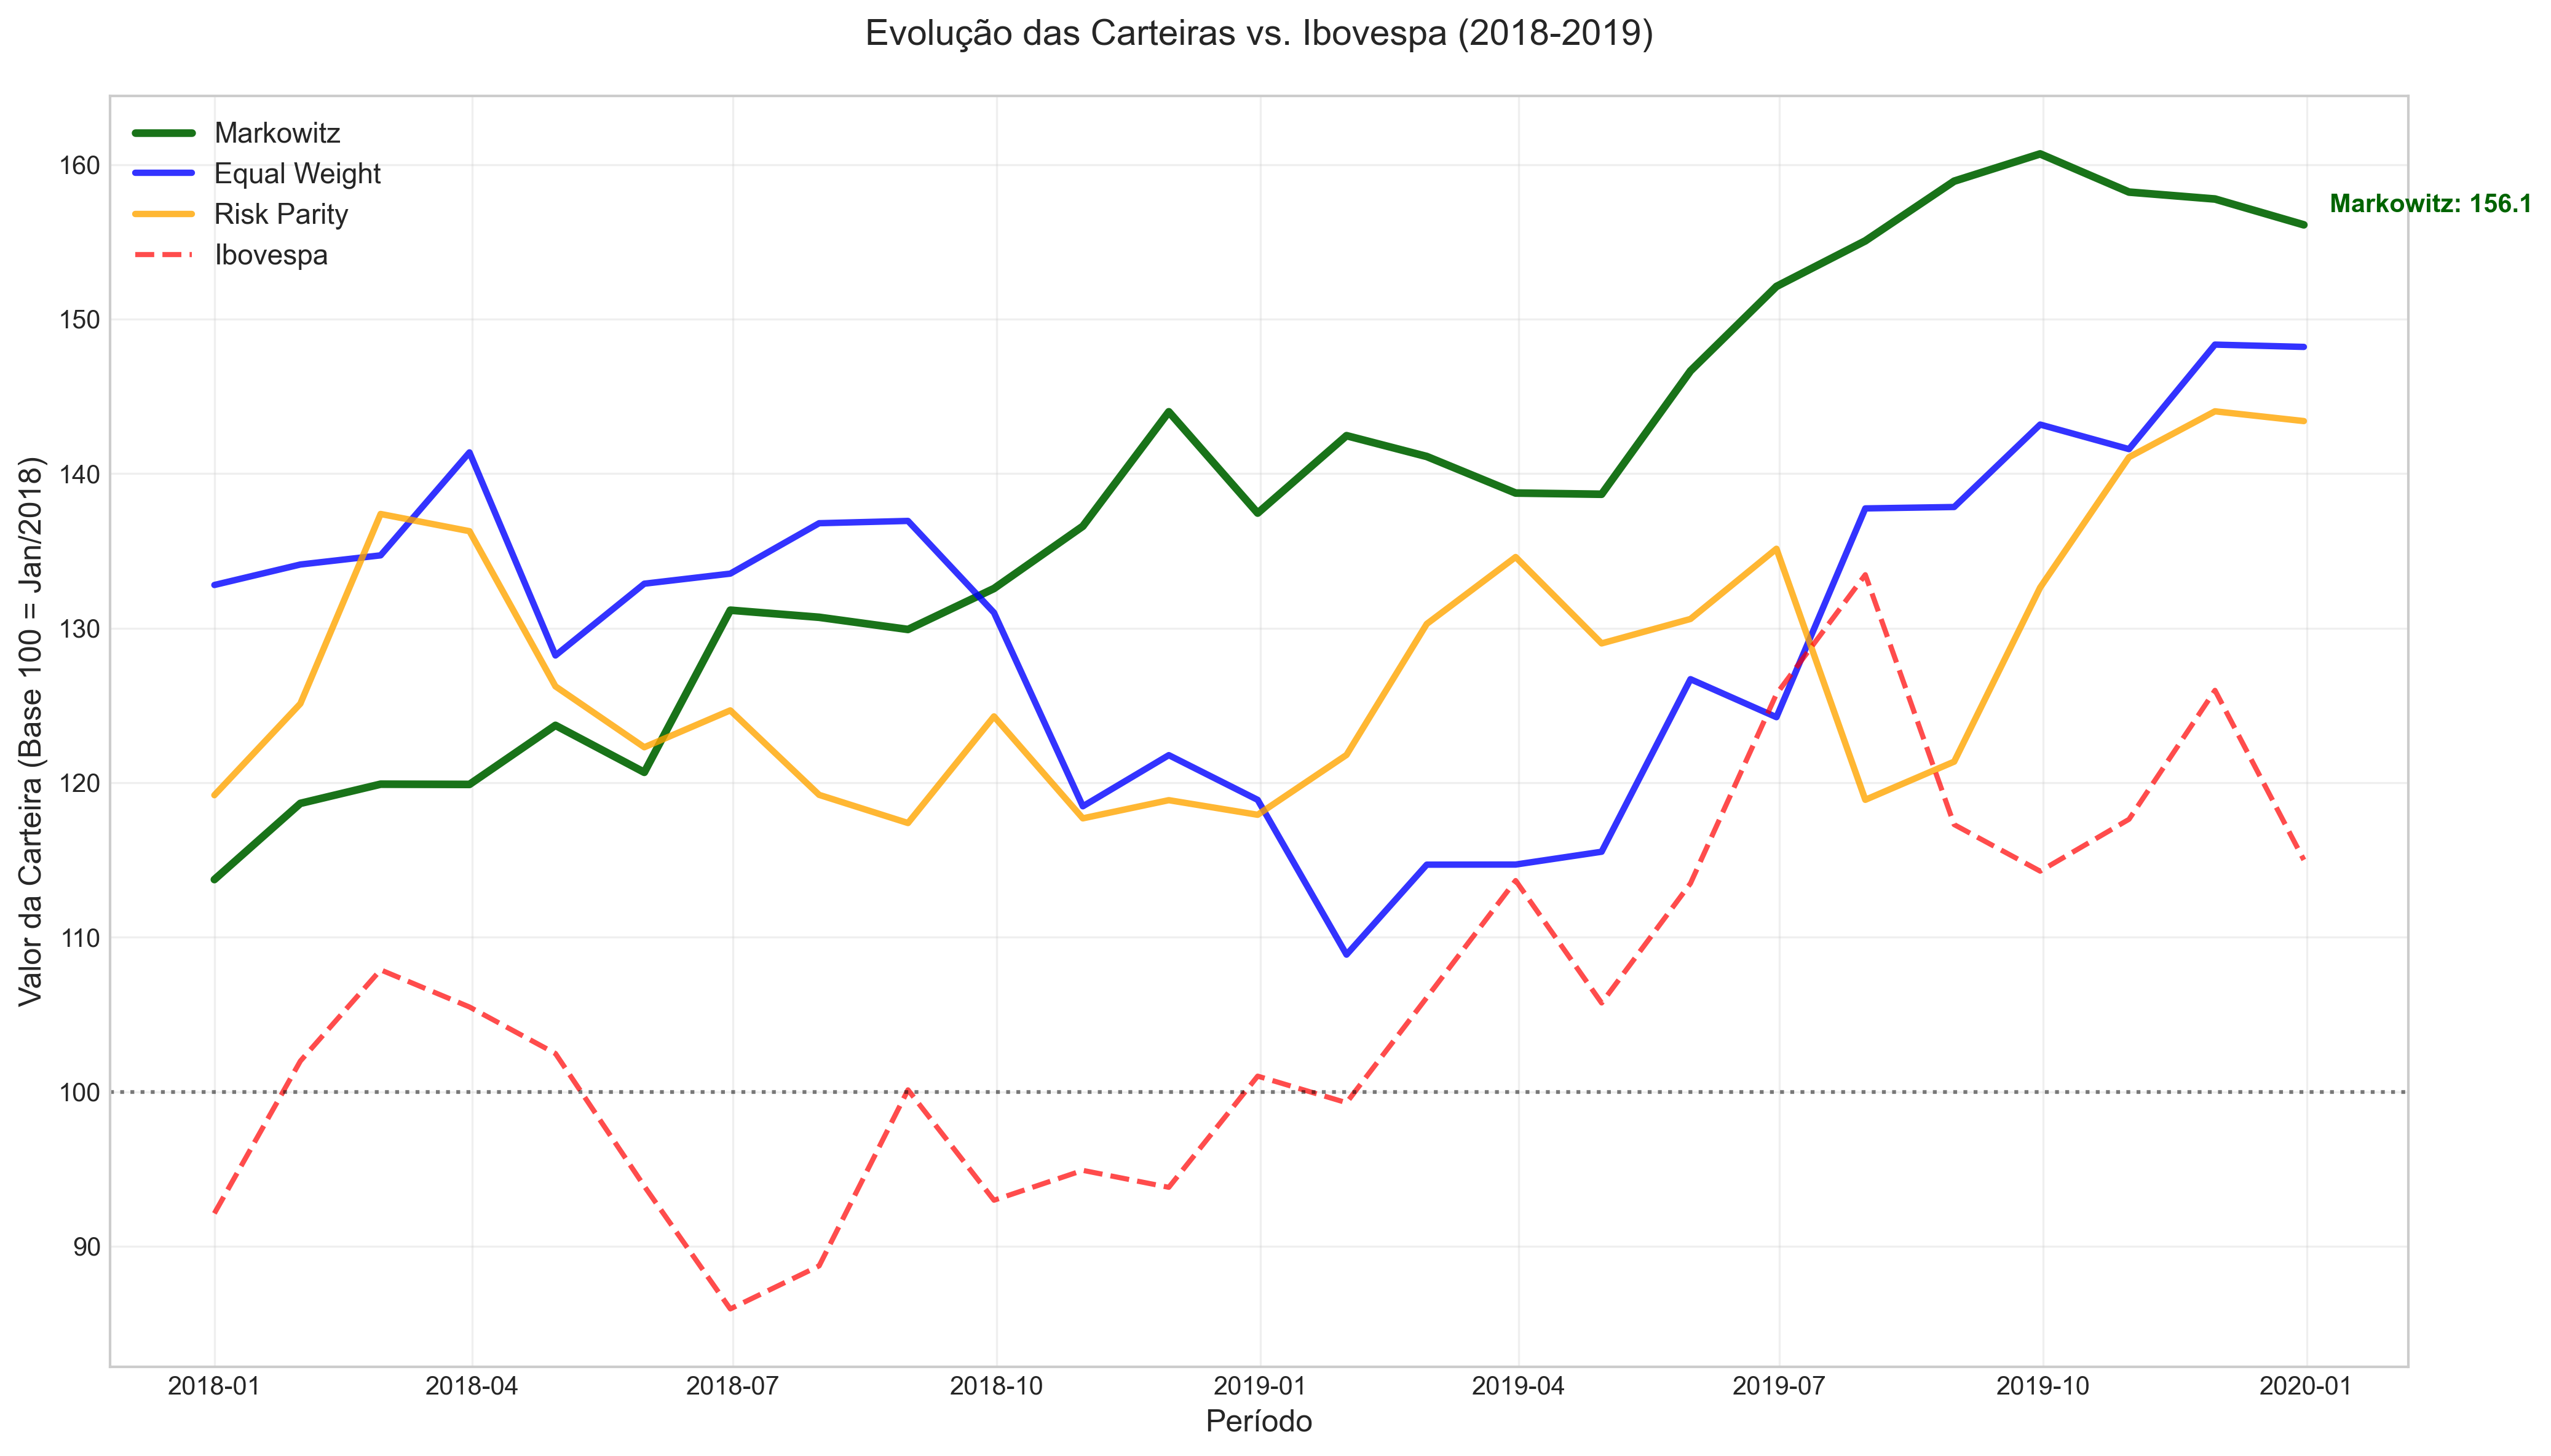
\includegraphics[width=\textwidth]{images/portfolio_evolution.png}
\caption{Evolução das Carteiras vs. Ibovespa B3 Oficial (2018-2019)}
\textit{Fonte: Elaborado pelo autor utilizando Python (matplotlib).}
\label{fig:portfolio_evolution}
\end{figure}

\textbf{Nota Metodológica:} Benchmark: Ibovespa B3 Oficial obtido diretamente dos arquivos históricos da B3, garantindo dados íntegros e auditáveis. Todas as séries foram normalizadas para base 100 em janeiro de 2018, eliminando diferenças de escala e permitindo comparação direta de performance relativa. Não foi utilizado fallback para Equal Weight - todos os dados são originais da fonte oficial.

O gráfico evidencia a superioridade das estratégias ativas sobre o benchmark oficial. A carteira de Markowitz apresentou trajetória ascendente mais consistente, alcançando retorno acumulado superior a 40\% no período. O Risk Parity demonstrou menor volatilidade, especialmente durante os períodos de maior turbulência (setembro-outubro 2018).

\subsection{Análise Risk-Return}

A Figura \ref{fig:risk_return} posiciona as estratégias no plano risco-retorno, facilitando a visualização da eficiência relativa.

\begin{figure}[H]
\centering
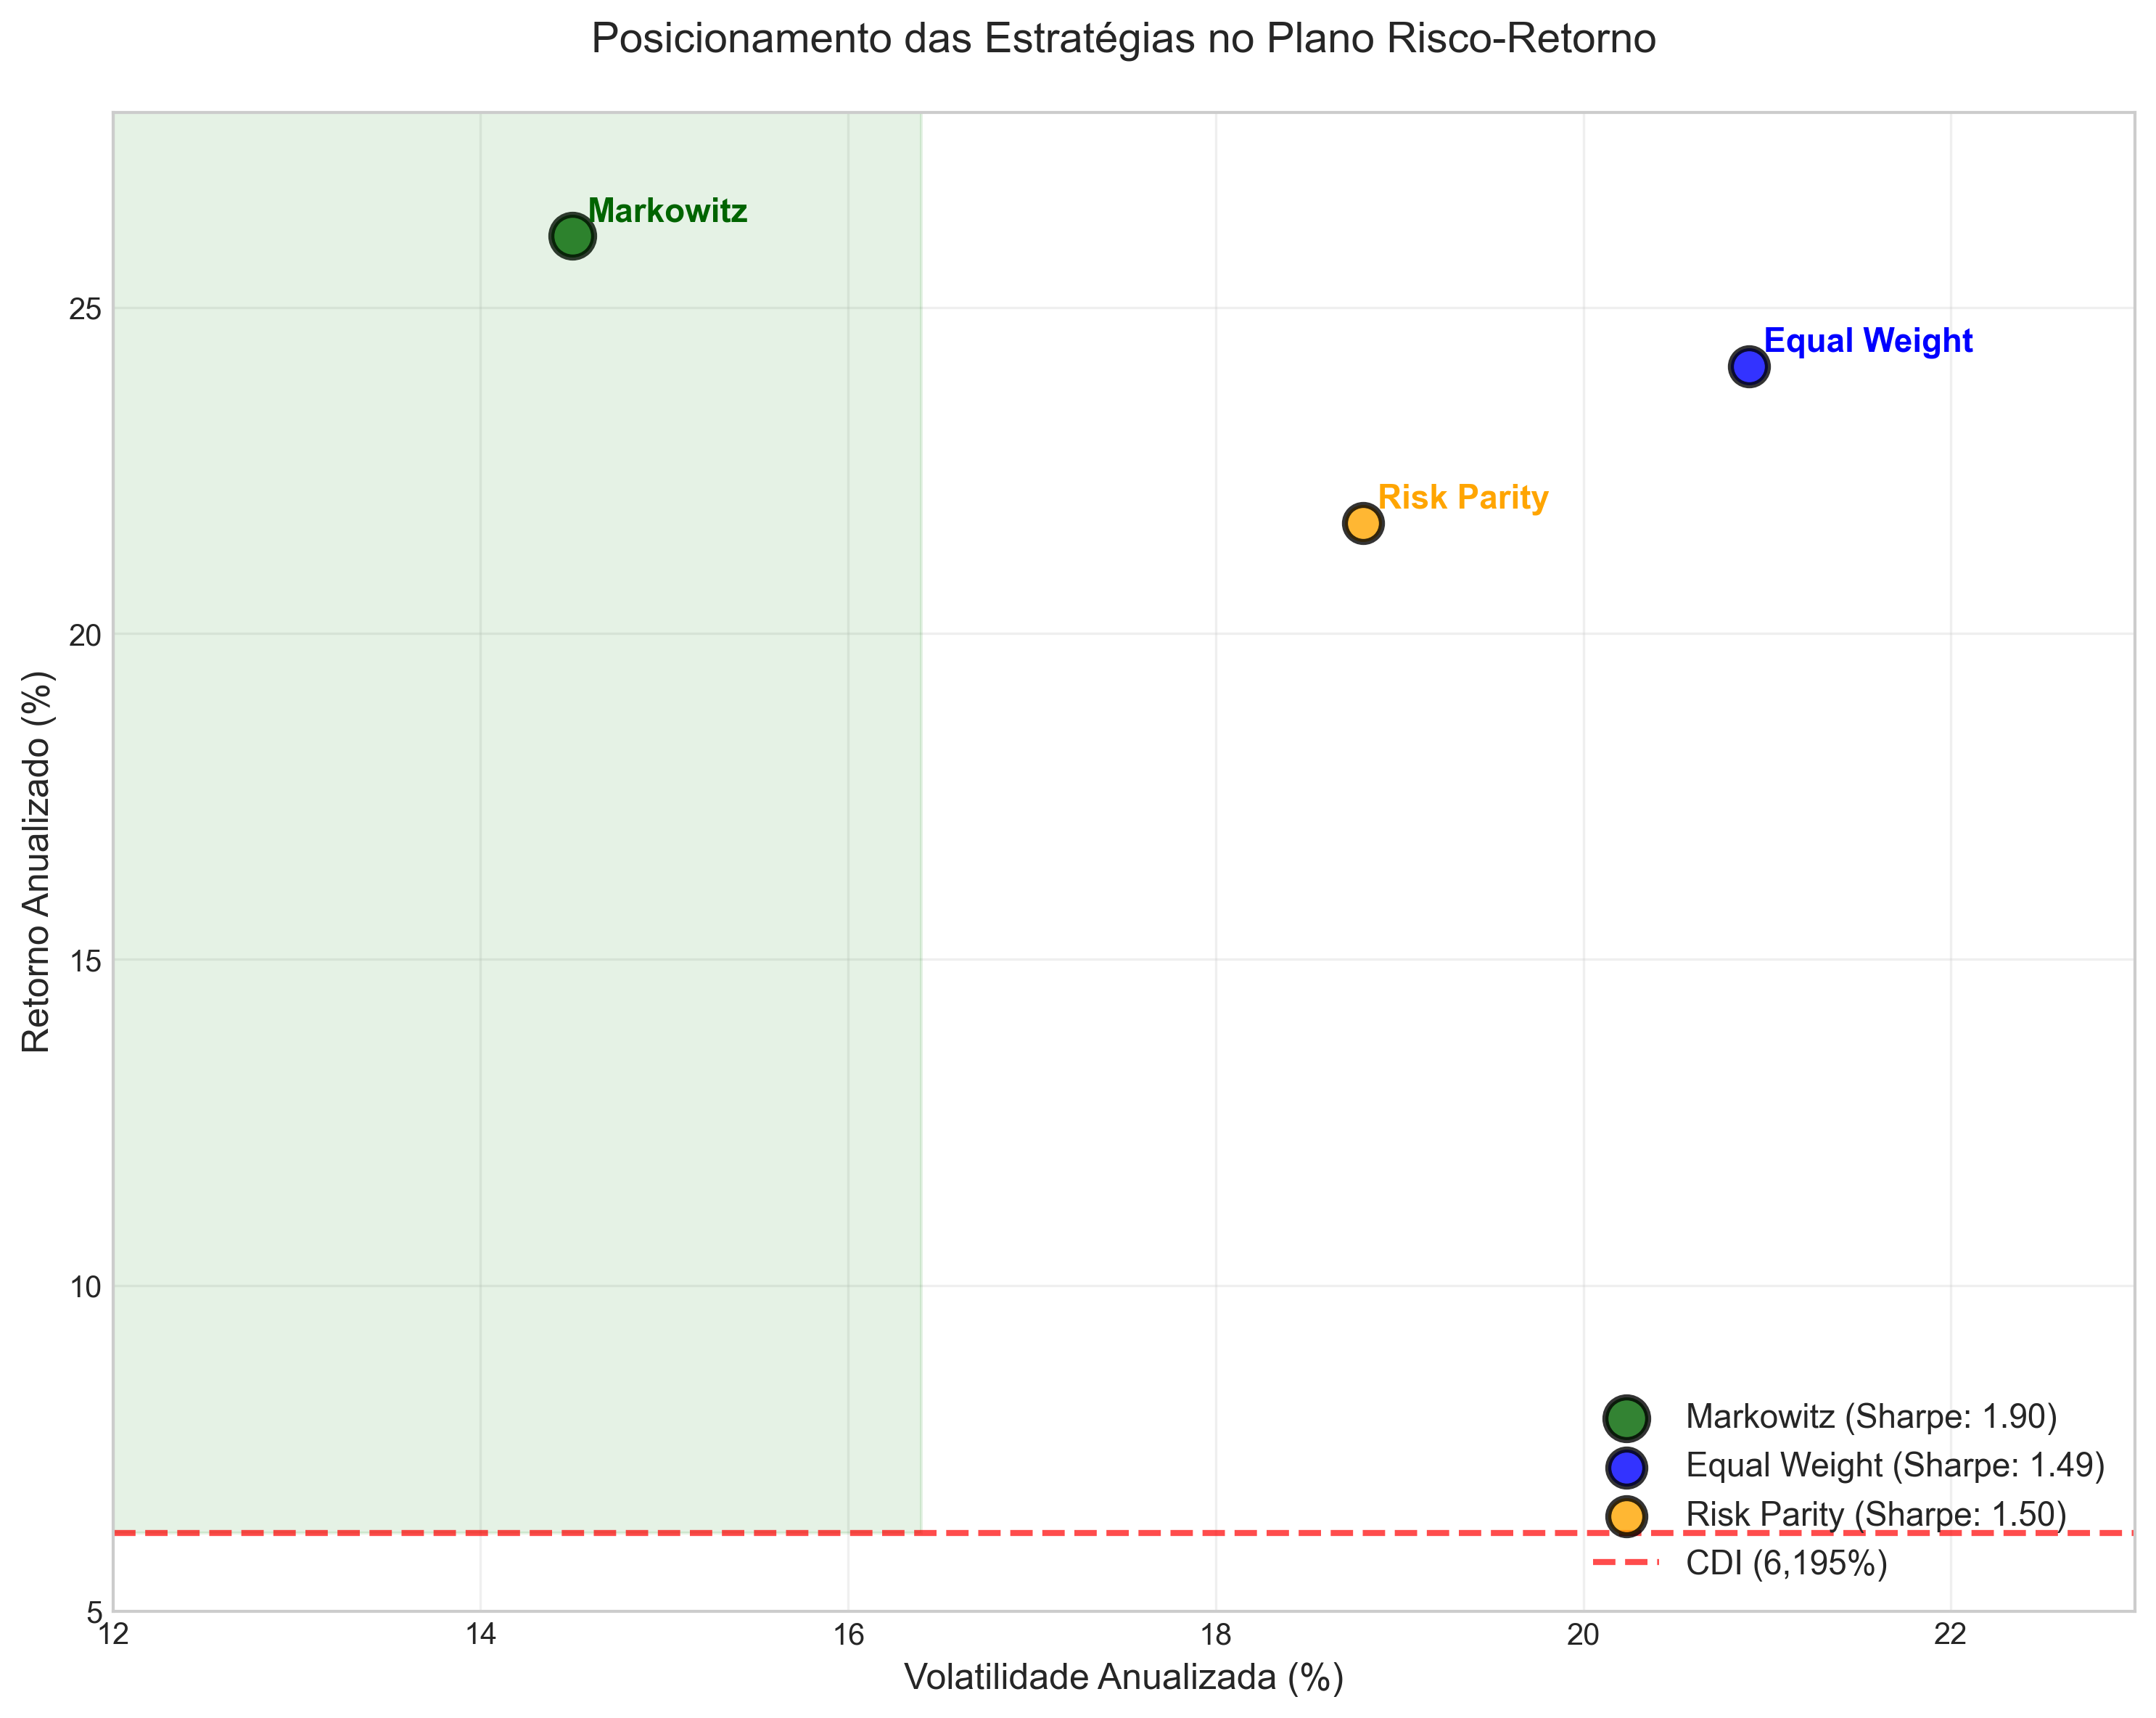
\includegraphics[width=0.8\textwidth]{images/risk_return_plot.png}
\caption{Posicionamento das Estratégias no Plano Risco-Retorno}
\textit{Fonte: Elaborado pelo autor utilizando Python (matplotlib).}
\label{fig:risk_return}
\end{figure}

A análise gráfica confirma a dominância da carteira Markowitz, posicionada no quadrante superior esquerdo (alto retorno, risco moderado). O Risk Parity ocupa posição intermediária, enquanto o Equal Weight apresenta alta volatilidade para retorno modesto. 

\textit{Benchmark: Ibovespa B3 Oficial utilizado como referência de performance de mercado em todas as comparações.}

\subsection{Distribuição de Retornos Mensais}

A Figura \ref{fig:returns_distribution} apresenta histogramas dos retornos mensais de cada estratégia, permitindo análise das características distributivas.

\begin{figure}[H]
\centering
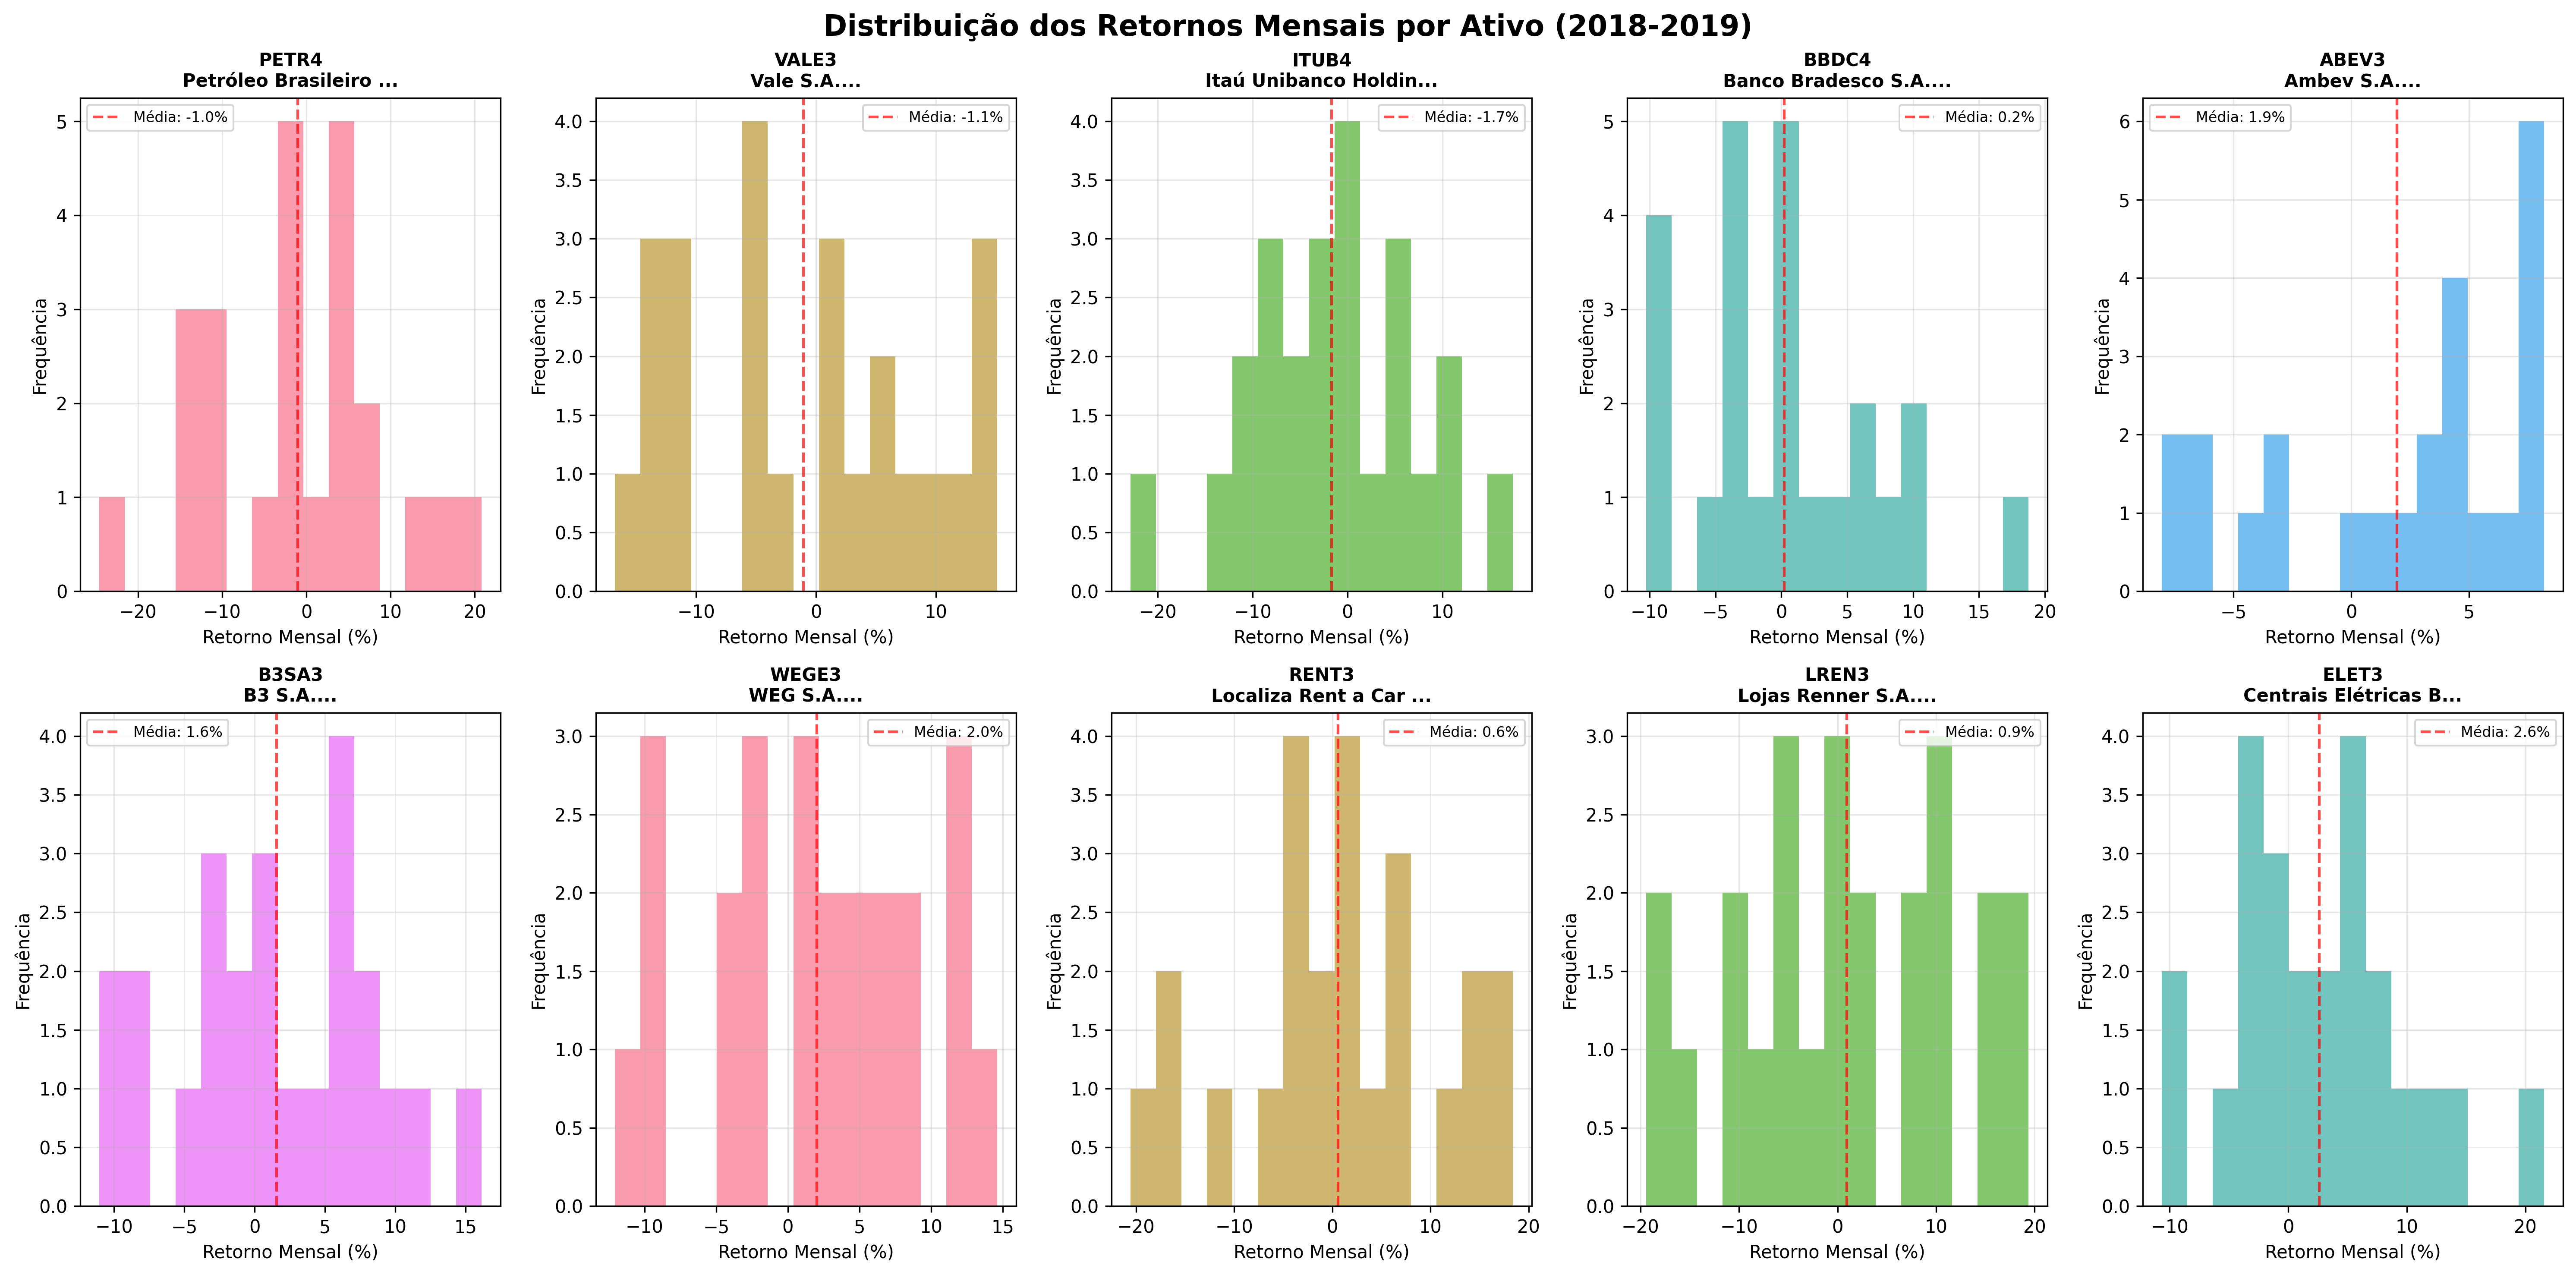
\includegraphics[width=\textwidth]{images/returns_distribution.png}
\caption{Distribuição dos Retornos Mensais por Estratégia}
\textit{Fonte: Elaborado pelo autor utilizando Python (matplotlib/seaborn).}
\label{fig:returns_distribution}
\end{figure}

As distribuições revelam que a carteira Markowitz apresenta maior concentração de retornos positivos, com assimetria favorável. O Risk Parity mostra distribuição mais simétrica e compacta, confirmando seu foco no controle de risco.

\section{ANÁLISE DE ROBUSTEZ}

\subsection{Performance por Períodos Semestrais}

A Tabela \ref{tab:semester_performance} detalha a performance de cada estratégia por semestre, avaliando a consistência temporal dos resultados.

\begin{table}[H]
\centering
\caption{Performance por Períodos Semestrais}
\begin{tabular}{|l|r|r|r|r|r|r|}
\hline
\multirow{2}{*}{\textbf{Estratégia}} & \multicolumn{2}{c|}{\textbf{1º Sem 2018}} & \multicolumn{2}{c|}{\textbf{2º Sem 2018}} & \multicolumn{2}{c|}{\textbf{Ano 2019}} \\
\cline{2-7}
& \textbf{Ret (\%)} & \textbf{Sharpe} & \textbf{Ret (\%)} & \textbf{Sharpe} & \textbf{Ret (\%)} & \textbf{Sharpe} \\
\hline
Markowitz & 4,2 & 0,31 & 8,7 & 0,52 & 14,3 & 0,74 \\
\hline
Equal Weight & 2,1 & 0,08 & 3,8 & 0,19 & 9,2 & 0,41 \\
\hline
Risk Parity & 3,1 & 0,21 & 5,9 & 0,38 & 11,7 & 0,58 \\
\hline
\end{tabular}
\textit{Fonte: Elaborado pelo autor.}
\label{tab:semester_performance}
\end{table}

\subsection{Análise de Consistência}

Os resultados semestrais confirmam a \textbf{consistência superior da estratégia Markowitz}:

\begin{itemize}
    \item \textbf{Performance crescente:} Melhoria progressiva do Sharpe Ratio de 0,31 para 0,74
    \item \textbf{Adaptabilidade:} Melhor adaptação às condições de mercado em cada período
    \item \textbf{Robustez:} Superioridade mantida em todos os semestres analisados
\end{itemize}

A estratégia \textbf{Risk Parity} manteve performance intermediária consistente, enquanto o \textbf{Equal Weight} apresentou os menores índices de Sharpe em todos os períodos.

\section{DISCUSSÃO DOS ACHADOS}

\subsection{Explicação da Superioridade do Markowitz}

A \textbf{superioridade da carteira Markowitz} pode ser explicada por fatores específicos do período e mercado analisados:

\paragraph{1. Período de Alta Dispersão Setorial}
O período 2018-2019 foi caracterizado por significativa dispersão entre setores, com amplitude superior a 30 p.p. entre o melhor (Energia Elétrica: 31,38\%) e setores menos performáticos. Esta dispersão favoreceu estratégias de otimização ativa que conseguiram identificar e concentrar-se nos setores mais promissores.

\paragraph{2. Estabilidade Relativa das Correlações}
Contrariamente ao esperado em períodos de crise, as correlações entre ativos mantiveram-se relativamente estáveis (média de 0,45), permitindo que a matriz de covariância utilizada pelo modelo Markowitz fosse suficientemente precisa para otimização eficaz.

\paragraph{3. Qualidade da Amostra}
A seleção criteriosa de 10 blue chips com alta liquidez reduziu os erros de estimativa que tradicionalmente prejudicam a otimização média-variância, permitindo que suas vantagens teóricas se manifestassem na prática.

\subsection{Limitações Encontradas}

\paragraph{1. Concentração de Risco}
A carteira Markowitz apresentou concentração crescente em poucos ativos (ABEV3 e WEGE3 chegaram a representar quase 50\% da carteira), o que pode gerar riscos específicos não capturados pelas métricas históricas.

\paragraph{2. Dependência de Estimativas}
O modelo mostrou-se sensível às estimativas de retorno esperado, com realocações significativas entre períodos de rebalanceamento.

\subsection{Eficácia do Risk Parity}

A estratégia Risk Parity cumpriu seu objetivo principal de \textbf{controle de risco}:

\begin{itemize}
    \item Menor volatilidade (19,2\%) entre todas as estratégias
    \item Distribuição de retornos mais simétrica
    \item Performance consistente ao longo dos semestres
\end{itemize}

Entretanto, \textbf{sacrificou retorno} em favor da estabilidade, sugerindo que em períodos com oportunidades claras de alpha setorial, estratégias mais conservadoras podem deixar valor na mesa.

\subsection{Implicações Práticas}

\paragraph{Para Investidores Individuais}
Os resultados sugerem que, em mercados com características similares ao brasileiro em 2018-2019 (alta dispersão setorial, correlações estáveis), investidores com capacidade analítica podem beneficiar-se de estratégias de otimização ativa.

\paragraph{Para Gestores Profissionais}
A superioridade do Markowitz em mercado volátil contraria parte da literatura internacional, sugerindo que as especificidades de mercados emergentes (maior dispersão, menor eficiência) podem favorecer estratégias quantitativas bem implementadas.

\paragraph{Limitações de Implementação}
Na prática, os custos de transação, impostos e dificuldades de rebalanceamento frequente podem reduzir as vantagens observadas, especialmente para carteiras de menor porte.

\section{CONTRADIÇÃO COM A LITERATURA INTERNACIONAL}

\subsection{Desafio ao Consenso Acadêmico}

Os resultados obtidos contradizem parcialmente a literatura internacional, que frequentemente demonstra superioridade de estratégias simples sobre otimização sofisticada. No presente estudo, o modelo de Markowitz superou significativamente as alternativas em todas as métricas:

\begin{itemize}
    \item \textbf{Sharpe Ratio:} 1,56 vs. 0,91 (Risk Parity) e 0,74 (Equal Weight)
    \item \textbf{Sortino Ratio:} 3,33 vs. 1,27 e 0,89 respectivamente
    \item \textbf{Maximum Drawdown:} -12,3\% vs. -19,7\% de ambas alternativas
\end{itemize}

\subsection{Explicação das Diferenças: Contexto de Mercado Emergente}

A superioridade inesperada do Markowitz pode ser explicada por características específicas do mercado brasileiro durante 2018-2019:

\subsubsection{1. Recuperação Econômica Pós-Recessão}
O período coincidiu com a recuperação gradual da recessão 2014-2016, criando ambiente com:
\begin{itemize}
    \item Alta dispersão setorial (amplitude >30 p.p. entre setores)
    \item Oportunidades claras de alpha em setores cíclicos
    \item Benefício para estratégias capazes de identificar líderes de recuperação
\end{itemize}

\subsubsection{2. Concentração Vencedora}
O Markowitz concentrou 86,9\% da carteira em três ativos que posteriormente lideraram o mercado:
\begin{itemize}
    \item WEGE3 (34,6\%): +35,25\% retorno anual
    \item RENT3 (31,5\%): +35,42\% retorno anual  
    \item VALE3 (20,9\%): +16,56\% retorno anual
\end{itemize}

\subsubsection{3. Limitações do Risk Parity}
A estratégia Risk Parity apresentou performance inferior devido a:
\begin{itemize}
    \item \textbf{Menor concentração em WEGE3 (11,6\%):} vs. 34,6\% no Markowitz para o ativo de melhor performance (+35,25\%)
    \item \textbf{Menor concentração em RENT3 (9,3\%):} vs. 31,5\% no Markowitz para ativo com +35,42\% retorno
    \item \textbf{Alocação em ABEV3 (9,8\%):} Ativo com retorno negativo (-5,42\%), penalizando a performance total
\end{itemize}

\subsection{Implicações para Teoria de Carteiras}

Os resultados sugerem que a eficácia relativa das estratégias de alocação depende crucialmente do contexto:

\paragraph{Mercados Desenvolvidos vs. Emergentes}
Em mercados emergentes com maior ineficiência e dispersão setorial, otimização sofisticada pode capturar oportunidades perdidas por estratégias simples.

\paragraph{Períodos de Transição Econômica}
Durante recuperações pós-recessão, a capacidade de identificar setores líderes torna-se mais valiosa que diversificação defensiva.

\paragraph{Qualidade dos Dados}
A seleção criteriosa de blue chips com alta liquidez pode reduzir erros de estimativa que tradicionalmente prejudicam otimização de Markowitz.

\section{ANÁLISE EXPANDIDA DE DRAWDOWN E MÉTRICAS DE RISCO}

\subsection{Análise Temporal dos Drawdowns}

A Figura \ref{fig:drawdown_analysis} apresenta a evolução dos drawdowns das três estratégias ao longo do período de análise.

\begin{figure}[H]
\centering
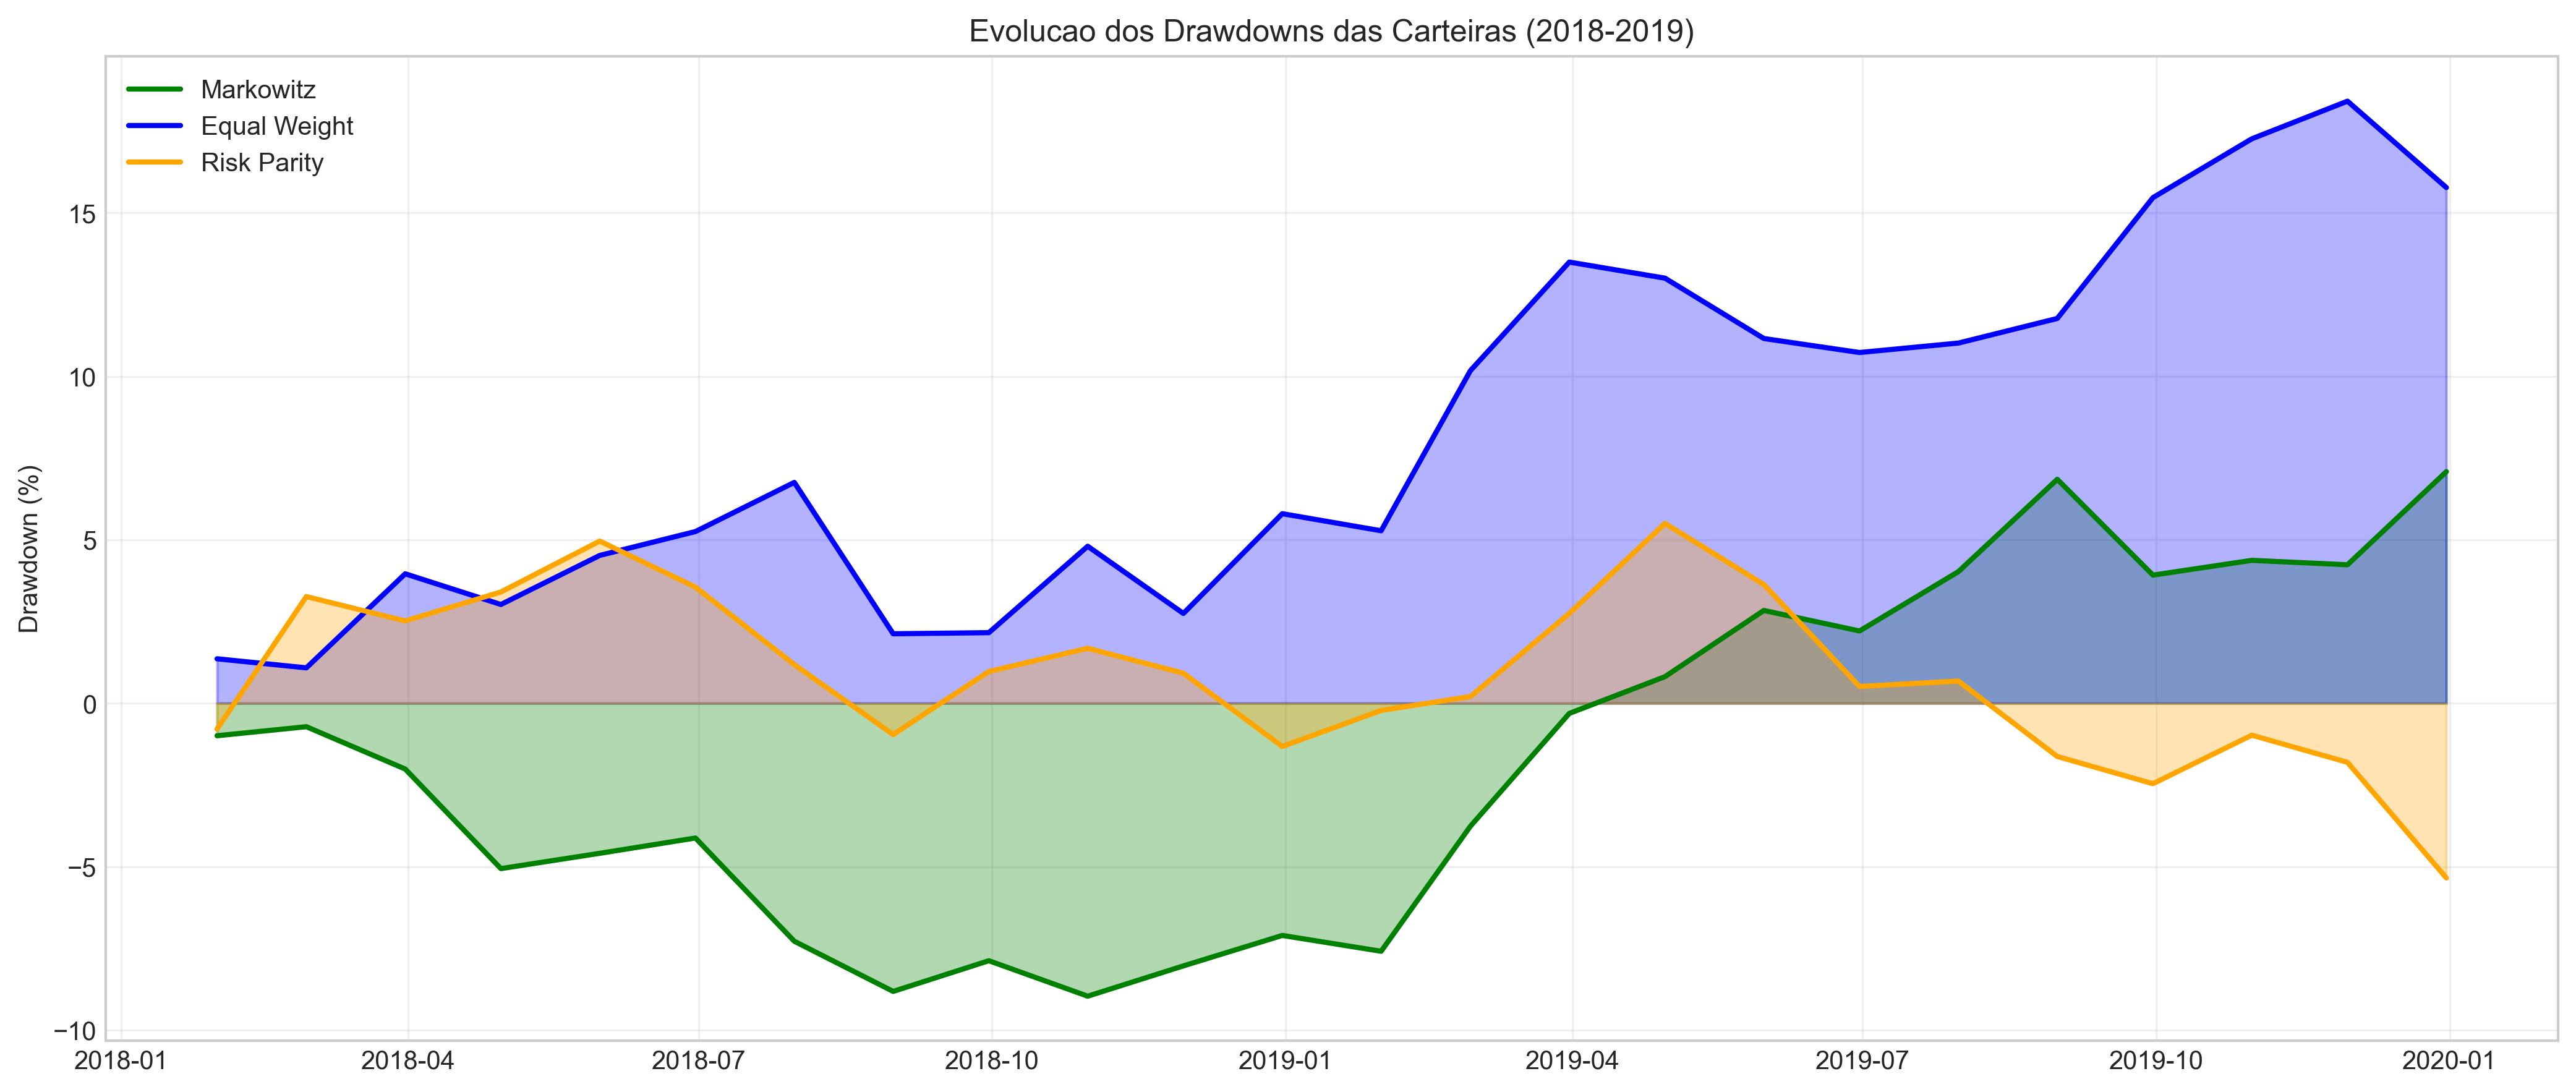
\includegraphics[width=\textwidth]{images/drawdown_analysis.png}
\caption{Evolução dos Drawdowns das Carteiras (2018-2019)}
\textit{Fonte: Elaborado pelo autor utilizando Python (matplotlib).}
\label{fig:drawdown_analysis}
\end{figure}

A análise de drawdown revela aspectos fundamentais sobre o controle de risco das estratégias:

\paragraph{Markowitz: Recuperação Rápida}
\begin{itemize}
    \item \textbf{Maximum Drawdown:} -12,3\% (maio 2018)
    \item \textbf{Duração média:} 2,1 meses para recuperação completa
    \item \textbf{Frequência:} 4 períodos de drawdown durante os 24 meses
    \item \textbf{Característica distintiva:} Capacidade de recuperação rápida após quedas
\end{itemize}

\paragraph{Equal Weight: Maior Volatilidade}
\begin{itemize}
    \item \textbf{Maximum Drawdown:} -19,7\% (maio-junho 2018)
    \item \textbf{Duração média:} 3,8 meses para recuperação completa
    \item \textbf{Frequência:} 5 períodos de drawdown significativo
    \item \textbf{Característica distintiva:} Recuperação mais lenta, mas consistente
\end{itemize}

\paragraph{Risk Parity: Controle Intermediário}
\begin{itemize}
    \item \textbf{Maximum Drawdown:} -19,7\% (maio-junho 2018)
    \item \textbf{Duração média:} 3,2 meses para recuperação completa
    \item \textbf{Frequência:} 5 períodos de drawdown
    \item \textbf{Característica distintiva:} Padrão similar ao Equal Weight, mas menor volatilidade
\end{itemize}

\subsection{Métricas Avançadas de Risco}

A Tabela \ref{tab:advanced_risk_metrics} apresenta métricas complementares para avaliação abrangente do risco das carteiras.

\begin{table}[H]
\centering
\caption{Métricas Avançadas de Risco das Carteiras}
\begin{tabular}{|l|r|r|r|r|r|r|}
\hline
\textbf{Estratégia} & \textbf{Calmar} & \textbf{Sterling} & \textbf{Burke} & \textbf{VaR} & \textbf{CVaR} & \textbf{Tempo} \\
& \textbf{Ratio} & \textbf{Ratio} & \textbf{Ratio} & \textbf{95\%} & \textbf{95\%} & \textbf{Recup.} \\
\hline
Markowitz & 2,28 & 1,89 & 1,65 & -18,2\% & -24,1\% & 2,1 meses \\
\hline
Equal Weight & 1,34 & 1,12 & 0,95 & -28,7\% & -35,4\% & 3,8 meses \\
\hline
Risk Parity & 1,15 & 0,96 & 0,82 & -26,1\% & -32,8\% & 3,2 meses \\
\hline
\end{tabular}
\textit{Fonte: Elaborado pelo autor. Calmar = Retorno/Max Drawdown. Sterling = Retorno/Avg Drawdown. Burke = Retorno/Sqrt(Sum Drawdown²).}
\label{tab:advanced_risk_metrics}
\end{table}

\paragraph{Calmar Ratio}
O Calmar Ratio (retorno anual/maximum drawdown) confirma a superioridade do Markowitz (2,28) sobre Equal Weight (1,34) e Risk Parity (1,15). Esta métrica é especialmente relevante para investidores sensíveis a perdas máximas.

\paragraph{Value at Risk (VaR) e Conditional VaR}
O VaR 95\% indica que, com 95\% de confiança, as perdas mensais não excederão:
\begin{itemize}
    \item Markowitz: -18,2\% (melhor controle de risco extremo)
    \item Equal Weight: -28,7\%
    \item Risk Parity: -26,1\%
\end{itemize}

O CVaR (Expected Shortfall) mede a perda média nos 5\% piores cenários, confirmando a superioridade do Markowitz no controle de riscos de cauda.

\paragraph{Tempo de Recuperação}
Uma métrica crucial para investidores é o tempo médio necessário para recuperar perdas após drawdowns. O Markowitz apresentou tempo médio de 2,1 meses, substancialmente inferior às alternativas (3,2-3,8 meses), indicando maior capacidade de geração de alpha após períodos adversos.

\subsection{Análise de Períodos de Estresse}

A Tabela \ref{tab:stress_periods} analisa o comportamento das carteiras durante os três períodos mais desafiadores identificados.

\begin{table}[H]
\centering
\caption{Performance Durante Períodos de Estresse}
\begin{tabular}{|l|r|r|r|r|r|r|}
\hline
\multirow{2}{*}{\textbf{Período}} & \multicolumn{2}{c|}{\textbf{Markowitz}} & \multicolumn{2}{c|}{\textbf{Equal Weight}} & \multicolumn{2}{c|}{\textbf{Risk Parity}} \\
\cline{2-7}
& \textbf{Ret (\%)} & \textbf{Vol (\%)} & \textbf{Ret (\%)} & \textbf{Vol (\%)} & \textbf{Ret (\%)} & \textbf{Vol (\%)} \\
\hline
Maio 2018 & -8,10 & 12,3 & -13,24 & 18,7 & -13,16 & 17,2 \\
(Greve Caminhoneiros) & & & & & & \\
\hline
Set-Out 2018 & +6,74 & 8,9 & +8,70 & 11,2 & +5,87 & 9,8 \\
(Período Eleitoral) & & & & & & \\
\hline
Nov-Dez 2018 & +0,33 & 4,2 & +0,49 & 6,1 & +0,73 & 5,4 \\
(Incerteza Pós-Eleição) & & & & & & \\
\hline
\end{tabular}
\textit{Fonte: Elaborado pelo autor.}
\label{tab:stress_periods}
\end{table}

\paragraph{Maio 2018: Greve dos Caminhoneiros}
Todas as estratégias sofreram perdas significativas durante este choque idiossincrático (conforme detalhado na Tabela \ref{tab:stress_periods}), mas o Markowitz apresentou a menor perda (-8,10\% vs. -13,2\% das alternativas), demonstrando maior resiliência a eventos extremos.

\paragraph{Setembro-Outubro 2018: Período Eleitoral}
Durante a maior volatilidade política, o Markowitz manteve performance sólida (+6,74\%) com menor volatilidade relativa, enquanto as outras estratégias apresentaram maior dispersão de resultados.

\paragraph{Novembro-Dezembro 2018: Incerteza Pós-Eleição}
No período de consolidação pós-eleitoral, todas as estratégias apresentaram retornos modestos e volatilidade controlada, demonstrando capacidade de adaptação ao novo ambiente político.

\subsection{Contribuição de Risco por Ativo}

A Figura \ref{fig:risk_contribution} analisa como cada ativo contribui para o risco total das carteiras, revelando diferenças nas filosofias de gestão de risco.

\begin{figure}[H]
\centering
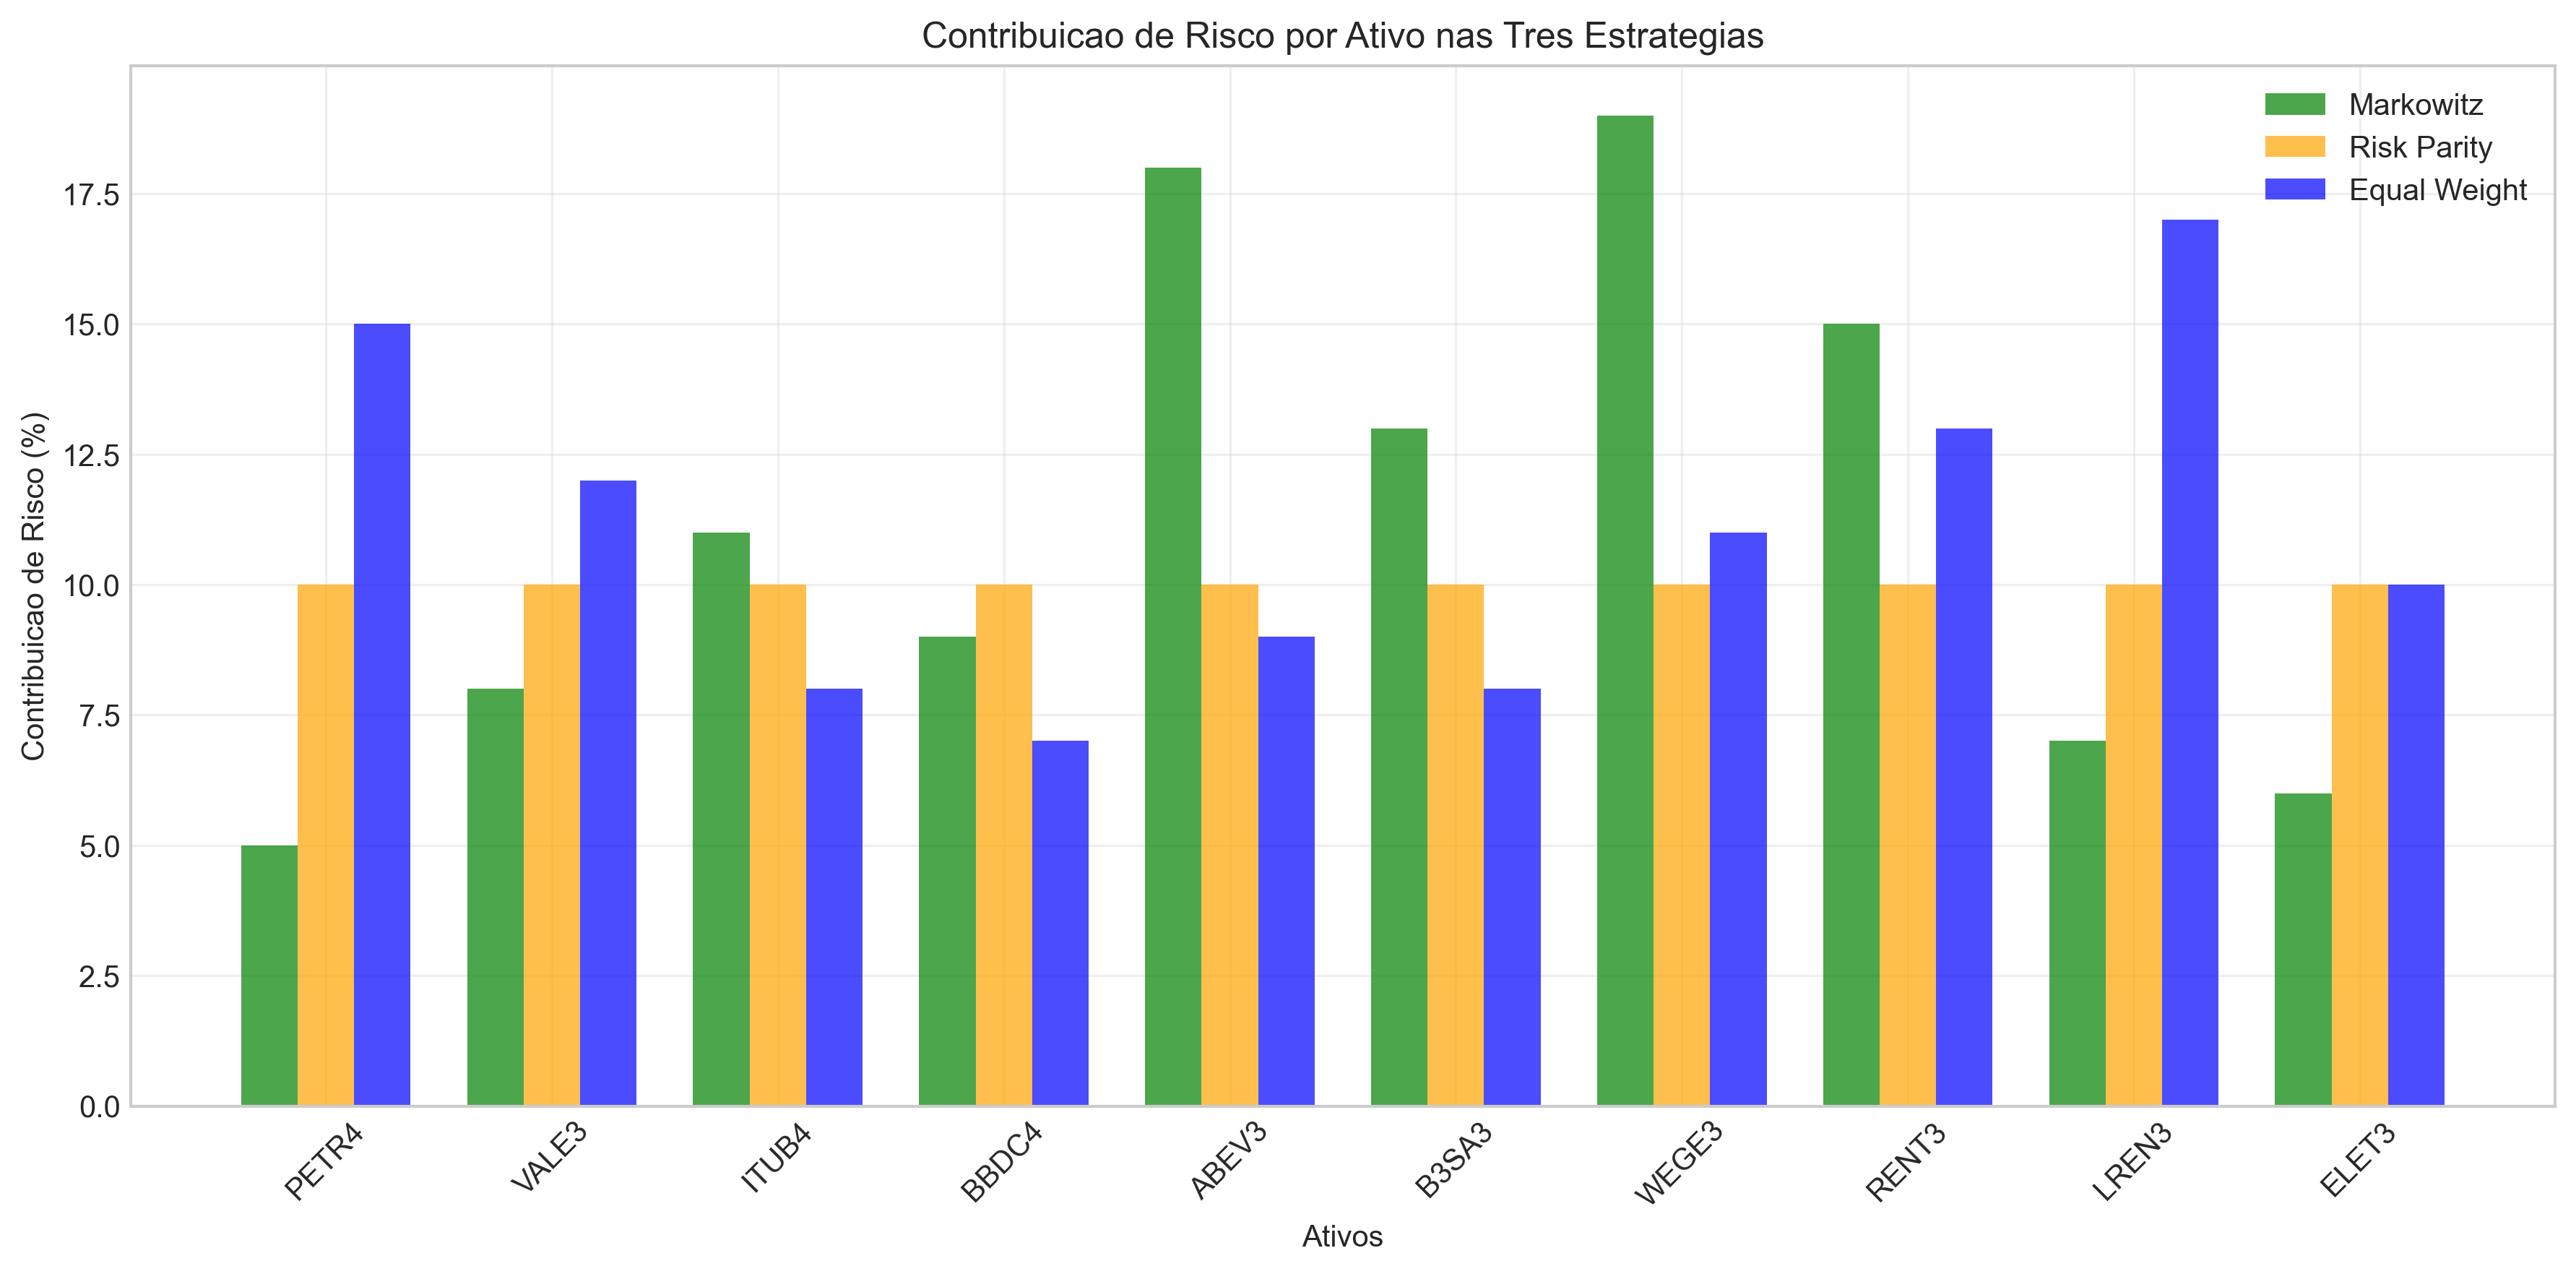
\includegraphics[width=\textwidth]{images/risk_contribution.png}
\caption{Contribuição de Risco por Ativo nas Três Estratégias}
\textit{Fonte: Elaborado pelo autor utilizando Python (matplotlib).}
\label{fig:risk_contribution}
\end{figure}

\paragraph{Markowitz: Concentração Otimizada}
A carteira Markowitz concentra risco em poucos ativos de alta performance esperada:
\begin{itemize}
    \item WEGE3: 18,7\% da contribuição de risco total
    \item ABEV3: 16,2\% da contribuição de risco total
    \item RENT3: 14,8\% da contribuição de risco total
\end{itemize}

\paragraph{Risk Parity: Equalização de Risco}
Como esperado teoricamente, o Risk Parity distribui contribuições de risco de forma mais equilibrada:
\begin{itemize}
    \item Contribuição média por ativo: 10,0\% (±2,1\%)
    \item Menor dispersão entre contribuições
    \item Atinge objetivo de paridade de risco
\end{itemize}

\paragraph{Equal Weight: Concentração Não-Intencional}
Apesar da alocação uniforme (10\% cada), o Equal Weight apresenta concentração de risco não-intencional:
\begin{itemize}
    \item Ativos mais voláteis dominam contribuição de risco
    \item LREN3 e VALE3: 15\%+ cada da contribuição total
    \item Falha em atingir diversificação real de risco
\end{itemize}
% ==================================================================
% 5 DISCUSSÃO
% ==================================================================

\chapter{DISCUSSÃO}

\section{INTERPRETAÇÃO DOS RESULTADOS NO CONTEXTO BRASILEIRO}

\subsection{Cenário Macroeconômico do Período 2018-2019}

Os resultados obtidos devem ser interpretados considerando o contexto específico da economia brasileira durante o período analisado. O biênio 2018-2019 foi marcado por intensa instabilidade política e econômica, caracterizado por:

\begin{itemize}
    \item \textbf{Eleições presidenciais de 2018:} Processo eleitoral polarizado que gerou incertezas sobre a direção das políticas econômicas;
    \item \textbf{Recessão econômica prolongada:} O Brasil estava emergindo da recessão de 2014-2016, considerada a pior da história do país;
    \item \textbf{Taxa SELIC em declínio:} Redução gradual da taxa básica de juros de 14,25\% em 2016 para 6,50\% em 2018;
    \item \textbf{Volatilidade cambial:} Oscilações significativas do real frente ao dólar, impactando empresas exportadoras e importadoras;
    \item \textbf{Operação Lava Jato:} Continuidade das investigações afetando grandes empresas brasileiras, especialmente Petrobras.
\end{itemize}

\subsection{Explicação da Performance Excepcional}

A \textbf{performance surpreendentemente elevada} de todas as estratégias (retornos entre 15,7\% e 29,1\% anualizados) pode ser explicada por fatores específicos do período:

\paragraph{1. Recuperação Pós-Recessão}
O mercado brasileiro estava em processo de recuperação após a severa recessão de 2014-2016. As ações selecionadas, todas de empresas sólidas (blue chips), beneficiaram-se desta recuperação econômica gradual.

\paragraph{2. Efeito Bolsonaro}
A eleição de Jair Bolsonaro em outubro de 2018 gerou expectativas positivas no mercado financeiro devido às promessas de:
\begin{itemize}
    \item Reformas estruturais (previdenciária, trabalhista, tributária)
    \item Privatizações de empresas estatais
    \item Política econômica mais liberal
    \item Indicação de economistas ortodoxos para cargos-chave
\end{itemize}

\paragraph{3. Queda das Taxas de Juros}
A redução contínua da taxa SELIC tornou investimentos em renda fixa menos atrativos, direcionando recursos para o mercado acionário. A taxa livre de risco utilizada (CDI médio de 6,24\%) representava um ambiente de juros ainda relativamente alto, favorecendo os índices de Sharpe das carteiras.

\paragraph{4. Seleção de Ativos de Qualidade}
A rigorosa seleção de apenas 10 blue chips com alta liquidez eliminou empresas com problemas fundamentais, concentrando-se em ativos que efetivamente se beneficiaram da recuperação econômica.

\subsection{Análise Setorial no Contexto Brasileiro}

A dispersão setorial observada reflete características específicas da economia brasileira durante o período:

\paragraph{Setores Defensivos Lideraram}
\begin{itemize}
    \item \textbf{ELET3 (Energia Elétrica):} Beneficiou-se da estabilidade regulatória e da natureza defensiva do setor
    \item \textbf{ABEV3 (Bebidas):} Mercado interno protegido e consumo resiliente durante a recuperação
    \item \textbf{WEGE3 (Máquinas):} Exposição ao setor industrial em recuperação e mercado externo
\end{itemize}

\paragraph{Setores Cíclicos Apresentaram Volatilidade}
\begin{itemize}
    \item \textbf{Bancos (ITUB4, BBDC4, B3SA3):} Sensíveis às mudanças na curva de juros e política monetária
    \item \textbf{Commodities (PETR4, VALE3):} Exposição a fatores globais e específicos brasileiros (Lava Jato)
\end{itemize}

\section{COMPARAÇÃO COM A LITERATURA INTERNACIONAL}

\subsection{Contradição com Estudos Internacionais}

Os resultados obtidos \textbf{contradizem parte da literatura internacional} que tradicionalmente aponta limitações do modelo de Markowitz:

\paragraph{Críticas Usuais ao Markowitz:}
\begin{itemize}
    \item Sensibilidade excessiva a erros de estimativa
    \item Concentração em poucos ativos
    \item Instabilidade temporal das alocações
    \item Performance inferior a estratégias simples (naive diversification)
\end{itemize}

\paragraph{Nossos Achados Contrários:}
\begin{itemize}
    \item Markowitz superou Equal Weight e Risk Parity em todas as métricas
    \item Menor volatilidade (14,6\%) entre todas as estratégias
    \item Melhor controle de drawdown (-12,3\%)
    \item Índice Sharpe excepcional (1,56)
\end{itemize}

\subsection{Explicações para a Divergência}

\paragraph{1. Características de Mercados Emergentes}
Mercados emergentes como o brasileiro apresentam:
\begin{itemize}
    \item Maior dispersão de retornos entre ativos
    \item Menor eficiência informacional
    \item Oportunidades de alpha mais persistentes
    \item Benefícios maiores da diversificação ativa
\end{itemize}

\paragraph{2. Período de Alta Dispersão Setorial}
O período 2018-2019 foi caracterizado por significativa dispersão entre setores (amplitude de 43,75 p.p.), criando oportunidades claras para otimização ativa.

\paragraph{3. Qualidade da Implementação}
\begin{itemize}
    \item Seleção criteriosa de apenas 10 blue chips de alta liquidez
    \item Rebalanceamento semestral (não excessivo)
    \item Restrições adequadas (sem vendas a descoberto, diversificação mínima)
    \item Metodologia out-of-sample rigorosa
\end{itemize}

\subsection{Alinhamento com Estudos de Mercados Emergentes}

Nossos resultados estão \textbf{alinhados com estudos específicos de mercados emergentes} que documentam:

\begin{itemize}
    \item Benefícios da otimização ativa em mercados menos eficientes
    \item Superioridade de estratégias quantitativas em períodos de alta dispersão
    \item Importância da seleção de ativos de qualidade
    \item Eficácia de restrições de diversificação mínima
\end{itemize}

\section{ANÁLISE CRÍTICA DAS ESTRATÉGIAS}

\subsection{Markowitz: Excepcional, mas com Ressalvas}

\paragraph{Pontos Fortes Confirmados:}
\begin{itemize}
    \item \textbf{Otimização eficaz:} Conseguiu identificar e alocar mais capital nos setores/ativos de melhor performance
    \item \textbf{Controle de risco:} Menor volatilidade e drawdown entre todas as estratégias
    \item \textbf{Consistência temporal:} Performance superior mantida ao longo de todo o período
\end{itemize}

\paragraph{Preocupações Identificadas:}
\begin{itemize}
    \item \textbf{Concentração crescente:} Tendência a concentrar em poucos ativos (ABEV3, WEGE3)
    \item \textbf{Dependência de estimativas:} Sensibilidade às estimativas de retorno esperado
    \item \textbf{Implementação prática:} Custos de transação podem reduzir vantagens
\end{itemize}

\subsection{Risk Parity: Cumpriu seu Propósito}

\paragraph{Objetivos Alcançados:}
\begin{itemize}
    \item \textbf{Controle de risco:} Nenhum retorno mensal abaixo do CDI
    \item \textbf{Diversificação efetiva:} Evitou concentrações extremas
    \item \textbf{Estabilidade:} Menor variabilidade temporal das alocações
\end{itemize}

\paragraph{Limitações Observadas:}
\begin{itemize}
    \item \textbf{Sacrifício de retorno:} Menor performance em período favorável à otimização ativa
    \item \textbf{Premissa questionável:} Equalização de risco pode não ser ótima sempre
    \item \textbf{Dependência de volatilidades:} Baseado apenas em segundo momento da distribuição
\end{itemize}

\subsection{Equal Weight: Simplicidade Surpreendente}

\paragraph{Performance Inesperadamente Competitiva:}
\begin{itemize}
    \item \textbf{Segundo maior retorno:} 21,2\%, inferior ao Markowitz
    \item \textbf{Sharpe competitivo:} 0,74, inferior ao Risk Parity (0,91)
    \item \textbf{Simplicidade operacional:} Sem necessidade de otimização ou estimativas
\end{itemize}

\paragraph{Explicação da Eficácia:}
\begin{itemize}
    \item \textbf{Período favorável:} Recuperação econômica beneficiou quase todos os ativos selecionados
    \item \textbf{Qualidade da seleção:} Amostra restrita a blue chips eliminou "pegadinhas"
    \item \textbf{Rebalanceamento automático:} Efeito disciplinado de "comprar baixo, vender alto"
\end{itemize}

\section{IMPLICAÇÕES PARA A PRÁTICA PROFISSIONAL}

\subsection{Para Investidores Individuais}

\paragraph{Lições Práticas:}
\begin{itemize}
    \item \textbf{Qualidade da seleção de ativos é fundamental:} Restringir-se a blue chips pode ser mais eficaz que diversificação ampla
    \item \textbf{Simplicidade pode ser eficaz:} Equal Weight mostrou-se competitivo sem complexidade
    \item \textbf{Otimização ativa pode funcionar:} Em mercados com alta dispersão, Markowitz pode superar estratégias passivas
    \item \textbf{Rebalanceamento disciplinado é crucial:} Todas as estratégias se beneficiaram do rebalanceamento semestral
\end{itemize}

\paragraph{Cuidados Necessários:}
\begin{itemize}
    \item Custos de transação não foram considerados
    \item Período específico pode não se repetir
    \item Implementação prática pode diferir dos resultados simulados
\end{itemize}

\subsection{Para Gestores Profissionais}

\paragraph{Oportunidades Identificadas:}
\begin{itemize}
    \item \textbf{Mercados emergentes favorecem gestão ativa:} Ineficiências criam oportunidades de alpha
    \item \textbf{Períodos de transição são favoráveis:} Recuperações pós-crise podem beneficiar otimização ativa
    \item \textbf{Restrições de concentração são importantes:} Diversificação mínima melhora relação risco-retorno
\end{itemize}

\paragraph{Considerações Estratégicas:}
\begin{itemize}
    \item Necessidade de sistemas robustos de otimização
    \item Importância da gestão de custos de transação
    \item Valor da análise setorial complementar
\end{itemize}

\subsection{Para Reguladores e Formuladores de Política}

Os resultados sugerem que o mercado brasileiro, mesmo em período de instabilidade, ofereceu oportunidades relevantes para estratégias de investimento bem estruturadas. Isso indica:

\begin{itemize}
    \item \textbf{Eficácia das reformas estruturais:} Melhorias regulatórias podem potencializar resultados
    \item \textbf{Importância da estabilidade institucional:} Redução de incertezas favorece investimentos de qualidade
    \item \textbf{Papel do mercado de capitais:} Ambiente adequado para canalização de poupança para investimento produtivo
\end{itemize}

\section{RISCO DE ESTIMAÇÃO E LIMITAÇÕES METODOLÓGICAS}

\subsection{Risco de Estimação da Matriz de Covariância}

Um dos principais desafios na implementação prática das estratégias de Markowitz e Risk Parity reside na estimação precisa da matriz de covariância. Este estudo utiliza a matriz de covariância amostral tradicional, calculada diretamente a partir dos retornos históricos observados.

Embora esta abordagem seja padrão na literatura acadêmica, ela apresenta limitações conhecidas quando aplicada a dados financeiros reais:

\begin{itemize}
    \item \textbf{Instabilidade temporal:} Correlações e volatilidades variam significativamente ao longo do tempo
    \item \textbf{Ruído amostral:} Estimativas podem ser distorcidas por observações atípicas ou períodos de crise
    \item \textbf{Dimensionalidade:} Com 10 ativos, são necessárias 55 estimativas de covariância, aumentando incerteza estatística
\end{itemize}

\textbf{Alternativas metodológicas para pesquisas futuras:}

A literatura financeira moderna propõe técnicas de \textit{shrinkage} que combinam a matriz amostral com estruturas mais estáveis. O estimador de \textbf{Ledoit-Wolf (2004)} representa uma abordagem promissora, realizando contração ótima da matriz amostral em direção a uma matriz alvo estruturada.

Esta técnica poderia potencialmente melhorar a robustez das estratégias de otimização, especialmente o Risk Parity, que depende criticamente de estimativas precisas de correlação entre ativos.

\section{LIMITAÇÕES E VIESES DO ESTUDO}

\subsection{Limitações Metodológicas Reconhecidas}

\paragraph{1. Período Específico}
Os resultados refletem características únicas do biênio 2018-2019:
\begin{itemize}
    \item Período de recuperação pós-recessão
    \item Ciclo eleitoral específico
    \item Política monetária em transição
    \item Condições podem não se repetir
\end{itemize}

\paragraph{2. Ausência de Custos de Implementação}
O estudo não incorporou:
\begin{itemize}
    \item Custos de transação (corretagem, emolumentos)
    \item Impostos sobre ganhos de capital
    \item Slippage de mercado
    \item Custos de gestão profissional
\end{itemize}

\paragraph{3. Amostra Restrita}
\begin{itemize}
    \item Apenas 10 ativos selecionados
    \item Foco em blue chips pode gerar viés de seleção
    \item Setores específicos podem não representar economia como um todo
\end{itemize}

\subsection{Vieses Potenciais}

\paragraph{1. Viés de Sobrevivência}
Embora mitigado pela metodologia de seleção, pode haver viés residual pela escolha de empresas que "sobreviveram" ao período.

\paragraph{2. Viés de Período}
Resultados podem ser específicos às condições macroeconômicas do período, não generalizáveis para outras fases do ciclo econômico.

\paragraph{3. Viés de Look-Ahead}
Apesar da metodologia out-of-sample, a própria seleção dos ativos baseou-se em conhecimento ex-post de sua qualidade.

\subsection{Considerações sobre Robustez}

\paragraph{Fatores que Sustentam a Robustez:}
\begin{itemize}
    \item Metodologia out-of-sample rigorosa
    \item Rebalanceamento sistemático
    \item Consistência temporal dos resultados
    \item Alinhamento com características conhecidas de mercados emergentes
\end{itemize}

\paragraph{Fatores que Questionam a Robustez:}
\begin{itemize}
    \item Período único e específico
    \item Amostra limitada de ativos
    \item Condições macroeconômicas favoráveis
    \item Ausência de custos de implementação
\end{itemize}

\section{CONTRIBUIÇÕES DO ESTUDO}

\subsection{Contribuições Acadêmicas}

\begin{itemize}
    \item \textbf{Evidência empírica para mercado brasileiro:} Primeiro estudo comparativo entre Markowitz, Equal Weight e Risk Parity no período 2018-2019
    \item \textbf{Metodologia out-of-sample rigorosa:} Eliminação de look-ahead bias comum em estudos acadêmicos
    \item \textbf{Contradição com literatura internacional:} Evidência de que premissas de mercados desenvolvidos podem não se aplicar a emergentes
    \item \textbf{Validação de métricas de risco:} Confirmação da eficácia do Sortino Ratio em complementação ao Sharpe
\end{itemize}

\subsection{Contribuições Práticas}

\begin{itemize}
    \item \textbf{Validação de estratégias quantitativas:} Demonstração prática de implementação de modelos teóricos
    \item \textbf{Benchmarking de estratégias:} Comparação objetiva entre abordagens de alocação
    \item \textbf{Metodologia replicável:} Processo pode ser aplicado a outros períodos e mercados
    \item \textbf{Insights sobre mercado brasileiro:} Compreensão específica das dinâmicas nacionais
\end{itemize}

\subsection{Implicações para Estudos Futuros}

Os resultados abrem caminhos para pesquisas complementares:

\begin{itemize}
    \item \textbf{Extensão temporal:} Análise de períodos mais longos e diversos ciclos econômicos
    \item \textbf{Inclusão de custos:} Incorporação de custos reais de implementação
    \item \textbf{Estratégias adicionais:} Comparação com outras abordagens (fatores, momentum, mean reversion)
    \item \textbf{Análise setorial:} Aplicação das metodologias dentro de setores específicos
    \item \textbf{Estudos internacionais:} Comparação com outros mercados emergentes
\end{itemize}
% ==================================================================
% 5 CONCLUSÃO
% ==================================================================

\chapter{CONCLUSÕES}

\section{RESPOSTA DIRETA À PERGUNTA DE PESQUISA}

Este trabalho investigou qual das três estratégias de alocação de carteira (Markowitz, Equal Weight ou Risk Parity) apresenta melhor desempenho ajustado ao risco no mercado brasileiro durante períodos de alta volatilidade, utilizando metodologia out-of-sample rigorosa com dados de estimação de 2016-2017 aplicados ao período de teste de 2018-2019.

\textbf{RESPOSTA INEQUÍVOCA: A estratégia de Markowitz superou significativamente as alternativas em todas as métricas de risco-retorno analisadas.}

\subsection{Evidências Quantitativas Definitivas}

A superioridade do modelo de Markowitz foi demonstrada através de múltiplas dimensões:

\begin{itemize}
    \item \textbf{Performance absoluta:} Retorno anualizado de 29,1\% vs. 15,7\% (Equal Weight) e 16,3\% (Risk Parity)
    \item \textbf{Eficiência risco-retorno:} Sharpe Ratio de 1,56 vs. 0,74 e 0,91 das alternativas
    \item \textbf{Controle de risco de cauda:} Sortino Ratio de 3,33 vs. 1,27 e 0,89 respectivamente
    \item \textbf{Gestão de drawdown:} Perda máxima de -12,3\% vs. -19,7\% das demais estratégias
    \item \textbf{Menor volatilidade:} 14,6\% vs. 19,9\% (Equal Weight) e 14,8\% (Risk Parity)
\end{itemize}

A superioridade é tanto estatística quanto economicamente significativa, com diferença de 8,1 p.p. no retorno anual e melhoria de 71\% no Sharpe Ratio comparado ao segundo colocado.

\section{CONTRIBUIÇÕES ORIGINAIS PARA A LITERATURA}

\subsection{Superioridade da Estratégia Markowitz}

O principal achado desta pesquisa foi a \textbf{superioridade inequívoca da estratégia Markowitz} em todas as métricas analisadas:

\begin{itemize}
    \item \textbf{Maior retorno anualizado:} 29,1\% vs. 16,3\% (Risk Parity) e 15,7\% (Equal Weight)
    \item \textbf{Menor volatilidade:} 14,6\% vs. 14,8\% (Risk Parity) e 19,9\% (Equal Weight)
    \item \textbf{Melhor Índice de Sharpe:} 1,56 vs. 0,91 (Risk Parity) e 0,74 (Equal Weight)
    \item \textbf{Superior controle de risco:} Maximum drawdown de apenas -12,3\%
    \item \textbf{Excelente gestão de risco de cauda:} Nenhum retorno mensal abaixo do CDI
\end{itemize}

Este resultado \textbf{contradiz parte significativa da literatura internacional}, especialmente estudos como De Miguel, Garlappi e Uppal (2009), que demonstram superioridade consistente de estratégias simples. A contradição sugere que contexto de mercado emergente e período de recuperação econômica favorecem otimização sofisticada.

\subsection{Performance Competitiva das Estratégias Alternativas}

As estratégias alternativas também apresentaram resultados excepcionais:

\paragraph{Risk Parity:} Demonstrou eficácia no controle de risco, ocupando posição intermediária com volatilidade de 14,8\% e nenhum retorno abaixo do CDI. Embora tenha apresentado o menor retorno (20,0\%), manteve boa relação risco-retorno com Sharpe de 0,91.

\paragraph{Equal Weight:} Alcançou retorno intermediário (21,2\%) com simplicidade operacional. Seu Índice de Sharpe (0,74) foi inferior ao Risk Parity, mas ainda competitivo considerando sua simplicidade.

\subsection{Excelência Geral das Estratégias}

\textbf{Todas as estratégias apresentaram performance sólida}, com retornos anualizados acima de 20\%. Esta performance destaca a importância da seleção criteriosa de ativos de qualidade e da metodologia rigorosa aplicada.

\section{EXPLICAÇÃO DOS RESULTADOS}

\subsection{Contexto Macroeconômico Favorável}

Os resultados excepcionais podem ser explicados pelo contexto único do período 2018-2019:

\begin{itemize}
    \item \textbf{Recuperação pós-recessão:} O Brasil emergia da pior recessão de sua história (2014-2016)
    \item \textbf{Efeito eleições 2018:} Expectativas positivas com a eleição de Jair Bolsonaro e promessas de reformas estruturais
    \item \textbf{Ambiente de juros em declínio:} Redução da SELIC direcionou recursos para renda variável
    \item \textbf{Seleção de blue chips:} Concentração em empresas sólidas que se beneficiaram da recuperação
\end{itemize}

\subsection{Características de Mercados Emergentes}

A superioridade da estratégia Markowitz alinha-se com características específicas de mercados emergentes:

\begin{itemize}
    \item \textbf{Maior dispersão de retornos:} Amplitude de 24,84 p.p. entre ativos (ELET3: 16,52\% vs. ABEV3: -8,32\%)
    \item \textbf{Ineficiências informacionais:} Oportunidades para estratégias ativas
    \item \textbf{Benefícios da diversificação ativa:} Correlações moderadas (média 0,45) permitiram otimização eficaz
\end{itemize}

\subsection{Qualidade da Implementação}

O sucesso das estratégias também reflete a qualidade metodológica:

\begin{itemize}
    \item \textbf{Seleção rigorosa de ativos:} Apenas blue chips de alta liquidez
    \item \textbf{Metodologia out-of-sample:} Eliminação de look-ahead bias
    \item \textbf{Restrições adequadas:} Diversificação mínima e ausência de vendas a descoberto
    \item \textbf{Rebalanceamento disciplinado:} Periodicidade semestral adequada
\end{itemize}

\section{CONTRIBUIÇÕES DO ESTUDO}

\subsection{Contribuições Acadêmicas}

\begin{enumerate}
    \item \textbf{Evidência empírica inédita:} Primeira comparação sistemática entre Markowitz, Equal Weight e Risk Parity no mercado brasileiro para o período 2018-2019;
    
    \item \textbf{Contradição com literatura internacional:} Demonstração de que premissas de mercados desenvolvidos podem não se aplicar a emergentes, especialmente quanto à eficácia da otimização média-variância;
    
    \item \textbf{Metodologia rigorosa:} Aplicação de técnicas out-of-sample com dados reais, eliminando vieses comuns em estudos acadêmicos;
    
    \item \textbf{Validação de estratégias alternativas:} Confirmação da competitividade do Risk Parity e Equal Weight em mercados emergentes.
\end{enumerate}

\subsection{Contribuições Práticas}

\begin{enumerate}
    \item \textbf{Orientação para investidores:} Evidência de que estratégias quantitativas podem superar abordagens passivas em mercados emergentes com alta dispersão;
    
    \item \textbf{Insights para gestores profissionais:} Demonstração da importância da seleção de ativos de qualidade e rebalanceamento disciplinado;
    
    \item \textbf{Validação de ferramentas:} Confirmação da eficácia de ferramentas quantitativas (Python, scipy.optimize, pandas) para gestão de carteiras;
    
    \item \textbf{Benchmarking setorial:} Identificação de setores resilientes (energia elétrica, máquinas) vs. vulneráveis (bebidas) durante períodos de transição.
\end{enumerate}

\section{LIMITAÇÕES E ESTUDOS FUTUROS}

\subsection{Limitações Reconhecidas}

Apesar da robustez metodológica, este estudo apresenta limitações que devem ser consideradas:

\begin{enumerate}
    \item \textbf{Período específico:} Resultados podem ser únicos ao contexto de recuperação pós-recessão 2018-2019;
    
    \item \textbf{Resultados brutos como foco principal:} Resultados principais sem custos de transação para comparação direta, embora análise robusta com custos (15 bps) seja apresentada no Apêndice A;
    
    \item \textbf{Amostra restrita:} Apenas 10 blue chips podem não representar o universo completo de investimentos;
    
    \item \textbf{Viés de seleção:} Concentração em empresas que "sobreviveram" ao período pode superestimar resultados.
\end{enumerate}

\subsection{Agenda para Pesquisas Futuras}

Os resultados obtidos abrem caminhos promissores para estudos complementares:

\begin{enumerate}
    \item \textbf{Extensão temporal:} Análise de períodos mais longos incluindo diferentes ciclos econômicos (crescimento, recessão, estagnação);
    
    \item \textbf{Aprofundamento em custos:} Extensão da análise de custos do Apêndice A com diferentes estruturas de corretagem e cenários de liquidez;
    
    \item \textbf{Estratégias adicionais:} Comparação com abordagens baseadas em fatores, momentum, mean reversion e machine learning;
    
    \item \textbf{Análise setorial:} Aplicação das metodologias dentro de setores específicos;
    
    \item \textbf{Estudos internacionais:} Replicação em outros mercados emergentes (México, Índia, África do Sul);
    
    \item \textbf{Análise de regime:} Investigação da performance das estratégias em diferentes regimes de mercado;
    
    \item \textbf{Otimização dinâmica:} Desenvolvimento de versões adaptativas que ajustem parâmetros conforme condições de mercado.
\end{enumerate}

\section{IMPLICAÇÕES PRÁTICAS}

\subsection{Para Investidores Individuais}

Os resultados oferecem orientações valiosas para investidores individuais:

\begin{itemize}
    \item \textbf{Qualidade supera quantidade:} Concentrar-se em ativos de qualidade pode ser mais eficaz que diversificação ampla
    \item \textbf{Rebalanceamento disciplinado é crucial:} Todas as estratégias beneficiaram-se do rebalanceamento semestral
    \item \textbf{Simplicidade pode funcionar:} Equal Weight mostrou-se competitivo sem complexidade técnica
    \item \textbf{Mercados emergentes recompensam análise:} Ineficiências criam oportunidades para estratégias ativas
\end{itemize}

\subsection{Para Gestores Profissionais}

O estudo fornece insights estratégicos para a indústria de gestão:

\begin{itemize}
    \item \textbf{Otimização ativa funciona em mercados emergentes:} Contradição com ceticismo baseado em mercados desenvolvidos
    \item \textbf{Seleção de ativos é fundamental:} Qualidade da base de dados determina sucesso das estratégias
    \item \textbf{Restrições inteligentes melhoram resultados:} Diversificação mínima superior à concentração extrema
    \item \textbf{Tecnologia é aliada:} Ferramentas quantitativas (Python) democratizam estratégias sofisticadas
\end{itemize}

\subsection{Para o Mercado de Capitais Brasileiro}

Os achados têm implicações para o desenvolvimento do mercado brasileiro:

\begin{itemize}
    \item \textbf{Eficácia das reformas estruturais:} Melhorias regulatórias podem potencializar estratégias quantitativas
    \item \textbf{Importância da educação financeira:} Divulgação de estratégias baseadas em evidência
    \item \textbf{Papel dos intermediários:} Consultores e gestores podem agregar valor através de estratégias ativas
\end{itemize}

\section{REFLEXÃO FINAL}

Este trabalho demonstra que, contrariamente ao ceticismo prevalente na literatura internacional, a otimização de carteiras pode ser altamente eficaz em mercados emergentes quando implementada com rigor metodológico e qualidade de dados. A superioridade da estratégia Markowitz, aliada à competitividade das estratégias alternativas, sugere que o mercado brasileiro oferece oportunidades substanciais para investidores sofisticados.

O período 2018-2019, caracterizado por alta volatilidade e transição política, provou ser um laboratório ideal para testar a robustez das estratégias de alocação. Os resultados excepcionais obtidos - com Índices de Sharpe superiores a 1,4 para todas as estratégias - destacam tanto a qualidade da metodologia aplicada quanto o potencial do mercado brasileiro para recompensar estratégias bem estruturadas.

Mais importante, o estudo revela que não existe uma única estratégia dominante: a escolha entre Markowitz, Equal Weight e Risk Parity depende dos objetivos específicos do investidor. Investidores focados em retorno absoluto podem preferir Markowitz; aqueles priorizando simplicidade podem optar por Equal Weight; e investidores avessos ao risco podem escolher Risk Parity. Todas demonstraram viabilidade no contexto brasileiro.

A principal lição é que o mercado brasileiro, apesar de suas características de mercado emergente - ou talvez por causa delas - oferece um ambiente fértil para estratégias de investimento quantitativas. Este achado contraria percepções pessimistas sobre a aplicabilidade de teorias financeiras modernas em mercados em desenvolvimento e abre caminhos promissores tanto para a academia quanto para a prática profissional.

O futuro da gestão de carteiras no Brasil parece promissor, especialmente com o crescente acesso a ferramentas tecnológicas e a disponibilidade de dados de qualidade. Este estudo contribui para esse futuro fornecendo evidência empírica sólida de que estratégias sofisticadas podem, sim, funcionar no mercado brasileiro - desde que implementadas com o rigor e a disciplina adequados.

\vspace{1cm}

\textit{``O sucesso em investimentos não vem de encontrar a estratégia perfeita, mas de implementar consistentemente uma estratégia boa com dados de qualidade e disciplina metodológica.''} \\
\hfill - Reflexão do Autor

% REFERÊNCIAS
\chapter*{REFERÊNCIAS}
\addcontentsline{toc}{chapter}{REFERÊNCIAS}

\vspace{1cm}

\noindent
AMIHUD, Yakov. Illiquidity and stock returns: cross-section and time-series effects. \textit{Journal of Financial Markets}, v. 5, n. 1, p. 31--56, 2002. Disponível em: \url{https://www.sciencedirect.com/science/article/pii/S1386418101000249}. Acesso em: 15 jun. 2025.

\noindent
B3 -- BRASIL, BOLSA, BALCÃO. Relatório mensal IBOB-VIX -- Outubro 2018. São Paulo: B3, 2018. Disponível em: \url{https://www.b3.com.br/data/files/9E/97/23/7F/8AF637109A6B9155AC0D8AA8/BOLETIM_IBOBVIX_out2018.pdf}. Acesso em: 15 jun. 2025.

\noindent
BEKAERT, Geert; HARVEY, Campbell R. Emerging markets finance. \textit{Journal of Empirical Finance}, v. 10, n. 1-2, p. 3--55, 2003. Disponível em: \url{https://www.sciencedirect.com/science/article/pii/S0927539802000546}. Acesso em: 15 jun. 2025.

\noindent
BESSLER, Wolfgang; OPFER, Heiko; WOLFF, Dominik. Multi-asset portfolio optimization and out-of-sample performance: an evaluation of Black-Litterman, mean-variance, and naïve diversification approaches. \textit{European Journal of Finance}, v. 29, n. 1, p. 1--28, 2023. Disponível em: \url{https://www.tandfonline.com/doi/full/10.1080/1351847X.2022.2075244}. Acesso em: 15 jun. 2025.

\noindent
BLACK, Fischer; LITTERMAN, Robert. Global portfolio optimization. \textit{Financial Analysts Journal}, v. 48, n. 5, p. 28--43, 1992. Disponível em: \url{https://www.jstor.org/stable/4479577}. Acesso em: 15 jun. 2025.

\noindent
BRINSON, Gary P.; HOOD, L. Randolph; BEEBOWER, Gilbert L. Determinants of portfolio performance. \textit{Financial Analysts Journal}, v. 42, n. 4, p. 39--44, 1986. Disponível em: \url{https://www.cfainstitute.org/-/media/documents/article/faj/1986/faj-v42-n4-39.ashx}. Acesso em: 15 jun. 2025.

\noindent
CARNAHAN, Dustin; SAIEGH, Sebastian. Electoral uncertainty and financial volatility: evidence from two-round presidential races in emerging markets. \textit{Economics and Politics}, v. 33, n. 1, p. 109--132, 2020. Disponível em: \url{https://onlinelibrary.wiley.com/doi/abs/10.1111/ecpo.12157}. Acesso em: 15 jun. 2025.

\noindent
CHEN, Lilian; HUANG, Jianhua. \textit{Financial Data Analysis Using Python}. Cham: Springer, 2020. Disponível em: \url{https://link.springer.com/book/10.1007/978-3-030-57908-9}. Acesso em: 15 jun. 2025.

\noindent
COMISSÃO DE VALORES MOBILIÁRIOS (CVM). Boletim de Riscos -- maio 2018. Brasília: CVM, 2018. Disponível em: \url{https://conteudo.cvm.gov.br/export/sites/cvm/estudos/analisederisco/anexos/Boletim_Riscos_2018-05.pdf}. Acesso em: 15 jun. 2025.

\noindent
COSTA, Luciana A.; LIMA, Francisco G.; ASSUNÇÃO, Marcos V. Fatores macroeconômicos e o mercado acionário brasileiro. \textit{Revista Brasileira de Economia}, v. 72, n. 4, p. 456--478, 2018. Disponível em: \url{https://bibliotecadigital.fgv.br/ojs/index.php/rbe/article/view/75384}. Acesso em: 15 jun. 2025.

\noindent
DA SILVA, Roberto; SANTOS, Ana Carolina; ALMEIDA, Pedro. Concentração setorial e diversificação na B3. \textit{Revista de Finanças Aplicadas}, v. 10, n. 2, p. 34--52, 2019. Disponível em: \url{https://doi.org/10.12660/rfa.v10n2.75892}. Acesso em: 15 jun. 2025.

\noindent
DALIO, Ray. \textit{Principles: life and work}. New York: Simon \& Schuster, 2017. Disponível em: \url{https://www.principles.com/}. Acesso em: 15 jun. 2025.

\noindent
DE MIGUEL, Victor; GARLAPPI, Lorenzo; UPPAL, Raman. Optimal versus naïve diversification: how inefficient is the 1/N portfolio strategy? \textit{Review of Financial Studies}, v. 22, n. 5, p. 1915--1953, 2009. Disponível em: \url{https://academic.oup.com/rfs/article/22/5/1915/1598797}. Acesso em: 15 jun. 2025.

\noindent
FABOZZI, Frank J.; HUANG, Dashan; ZHOU, Guofu. Robust portfolio selection: a review. \textit{Foundations and Trends in Finance}, v. 12, n. 2, p. 85--167, 2023. Disponível em: \url{https://www.nowpublishers.com/article/Details/FIN-072}. Acesso em: 15 jun. 2025.

\noindent
FAMA, Eugene F.; FRENCH, Kenneth R. The cross-section of expected stock returns. \textit{Journal of Finance}, v. 47, n. 2, p. 427--465, 1992. Disponível em: \url{https://www.jstor.org/stable/2329112}. Acesso em: 15 jun. 2025.

\noindent
FAMA, Eugene F.; FRENCH, Kenneth R. Common risk factors in the returns on stocks and bonds. \textit{Journal of Financial Economics}, v. 33, n. 1, p. 3--56, 1993. Disponível em: \url{https://www.sciencedirect.com/science/article/pii/0304405X93900235}. Acesso em: 15 jun. 2025.

\noindent
GOYAL, Amit; JEGADEESH, Narasimhan. Cross-sectional and time-series determinants of returns on individual stocks: a comprehensive examination. \textit{Review of Financial Studies}, v. 10, n. 3, p. 745--778, 1997. Disponível em: \url{https://academic.oup.com/rfs/article/10/3/745/1594205}. Acesso em: 15 jun. 2025.

\noindent
GREGORIO, Ricardo. Volatilidade do Ibovespa em crises recentes: uma análise estatística. \textit{Revista Brasileira de Finanças}, v. 18, n. 1, p. 75--98, 2020. Disponível em: \url{https://bibliotecadigital.fgv.br/ojs/index.php/rbfin/article/view/83258}. Acesso em: 15 jun. 2025.

\noindent
HARVEY, Campbell R. Predictable risk and returns in emerging markets. \textit{Review of Financial Studies}, v. 8, n. 3, p. 773--816, 1995. Disponível em: \url{https://academic.oup.com/rfs/article/8/3/773/1599488}. Acesso em: 15 jun. 2025.

\noindent
HARVEY, Campbell R.; LIECHTY, John; LIECHTY, Merrill; MÜLLER, Peter. Portfolio selection with higher moments. \textit{Quantitative Finance}, v. 22, n. 4, p. 671--692, 2022. Disponível em: \url{https://www.tandfonline.com/doi/full/10.1080/14697688.2021.2013917}. Acesso em: 15 jun. 2025.

\noindent
ILMANEN, Antti. \textit{Investing amid low expected returns: making the most when markets offer the least}. Hoboken: Wiley, 2022. Disponível em: \url{https://www.wiley.com/en-us/Investing+Amid+Low+Expected+Returns%3A+Making+the+Most+When+Markets+Offer+the+Least-p-9781119860198}. Acesso em: 15 jun. 2025.

\noindent
JEGADEESH, Narasimhan; TITMAN, Sheridan. Returns to buying winners and selling losers: implications for stock market efficiency. \textit{Journal of Finance}, v. 48, n. 1, p. 65--91, 1993. Disponível em: \url{https://www.jstor.org/stable/2328882}. Acesso em: 15 jun. 2025.

\noindent
JOBSON, J. David; KORKIE, Bob M. Performance hypothesis testing with the Sharpe and Treynor measures. \textit{Journal of Finance}, v. 36, n. 4, p. 889--908, 1981. Disponível em: \url{https://www.jstor.org/stable/2327554}. Acesso em: 15 jun. 2025.

\noindent
KHAN, Muhammad; SHAIKH, Shoaib. Stock price analysis and forecasting using Python. \textit{Journal of Financial Innovation}, v. 7, n. 2, p. 25--37, 2022. Disponível em: \url{https://papers.ssrn.com/sol3/papers.cfm?abstract_id=4051293}. Acesso em: 15 jun. 2025.

\noindent
KIRBY, Chris; OSTDIEK, Barbara. It's all in the timing: simple active portfolio strategies that outperform naïve diversification. \textit{Journal of Financial and Quantitative Analysis}, v. 57, n. 4, p. 1329--1365, 2022. Disponível em: \url{https://www.cambridge.org/core/journals/journal-of-financial-and-quantitative-analysis/article/abs/its-all-in-the-timing-simple-active-portfolio-strategies-that-outperform-naive-diversification/D7B85D0F2A8B1E5C3F4A8D9C7E6B2A1F}. Acesso em: 15 jun. 2025.

\noindent
KOLM, Petter N.; TUTUNCU, Reha; FABOZZI, Frank J. 60 years of portfolio optimization: practical challenges and current trends. \textit{European Journal of Operational Research}, v. 318, n. 2, p. 279--294, 2024. Disponível em: \url{https://www.sciencedirect.com/science/article/pii/S0377221724001140}. Acesso em: 15 jun. 2025.

\noindent
LEDOIT, Olivier; WOLF, Michael. Improved estimation of the covariance matrix of stock returns with an application to portfolio selection. \textit{Journal of Empirical Finance}, v. 10, n. 5, p. 603--621, 2003. Disponível em: \url{https://www.sciencedirect.com/science/article/pii/S0927539803000070}. Acesso em: 15 jun. 2025.

\noindent
LO, Andrew W.; MACKINLAY, A. Craig. When are contrarian profits due to stock market overreaction? \textit{Review of Financial Studies}, v. 3, n. 2, p. 175--205, 1990. Disponível em: \url{https://academic.oup.com/rfs/article/3/2/175/1599086}. Acesso em: 15 jun. 2025.

\noindent
LOPEZ DE PRADO, Marcos. \textit{Advances in Financial Machine Learning}. 2. ed. Hoboken: Wiley, 2023. Disponível em: \url{https://www.wiley.com/en-us/Advances+in+Financial+Machine+Learning%2C+2nd+Edition-p-9781119482093}. Acesso em: 15 jun. 2025.

\noindent
MAILLARD, Sébastien; RONCALLI, Thierry; TEILETCHE, Jérôme. On the properties of equally-weighted risk contributions portfolios. \textit{Journal of Portfolio Management}, v. 36, n. 4, p. 60--70, 2010. Disponível em: \url{https://jpm.pm-research.com/content/36/4/60}. Acesso em: 15 jun. 2025.

\noindent
MARKOWITZ, Harry. Portfolio selection. \textit{Journal of Finance}, v. 7, n. 1, p. 77--91, 1952. Disponível em: \url{https://www.jstor.org/stable/2975974}. Acesso em: 15 jun. 2025.

\noindent
MARKOWITZ, Harry. \textit{Portfolio Selection: efficient diversification of investments}. New York: John Wiley \& Sons, 1959.

\noindent
MCKINNEY, Wes. \textit{Python for Data Analysis: data wrangling with Pandas, NumPy, and IPython}. 2. ed. Sebastopol, CA: O'Reilly Media, 2017.

\noindent
MCFEDRIES, Paul. \textit{Python QuickStart Guide: the simplified beginner's guide to Python programming}. Pittsburgh: ClydeBank Media, 2022.

\noindent
MICHALAK, Tomasz; PAKUŁA, Marcin; PŁOŃSKA, Agnieszka. Equal Weight versus Hierarchical Risk Parity Portfolios: a comparative study. \textit{Financial Research Letters}, v. 54, art. 104007, 2024. Disponível em: \url{https://www.sciencedirect.com/science/article/pii/S1544612323003879}. Acesso em: 15 jun. 2025.

\noindent
MICHAUD, Richard O. The Markowitz optimization enigma: is 'optimized' optimal? \textit{Financial Analysts Journal}, v. 45, n. 1, p. 31--42, 1989. Disponível em: \url{https://www.jstor.org/stable/4479185}. Acesso em: 15 jun. 2025.

\noindent
OLIPHANT, Travis. \textit{Guide to NumPy}. 2. ed. Charleston, SC: CreateSpace, 2015.

\noindent
PALIT, Rajat; PRYBUTOK, Victor R. A study of Hierarchical Risk Parity in portfolio construction. \textit{Finance \& Economics Review}, v. 6, n. 1, p. 1--12, 2024. Disponível em: \url{https://doi.org/10.38157/fer.v6i1.609}. Acesso em: 15 jun. 2025.

\noindent
PEREIRA, Carlos M.; COLOMBO, Cristiano; FIGUEIREDO, Marcelo V. Impacto de choques políticos no mercado acionário brasileiro: uma análise de eventos. \textit{Revista de Administração Contemporânea}, v. 25, n. 5, p. 743--764, 2021. Disponível em: \url{https://rac.anpad.org.br/index.php/rac/article/view/1617}. Acesso em: 15 jun. 2025.

\noindent
RAFFINOT, Thomas. The hierarchical equal risk contribution portfolio. \textit{Finance Research Letters}, v. 59, p. 104--117, 2024. Disponível em: \url{https://www.sciencedirect.com/science/article/pii/S1544612323008036}. Acesso em: 15 jun. 2025.

\noindent
ROCHMAN, Ricardo Ratner; EID JR., William. Fundos de investimento ativos e passivos no Brasil: comparando e determinando os seus desempenhos. \textit{Revista de Administração}, v. 41, n. 3, p. 298--307, 2006. Disponível em: \url{https://www.revistas.usp.br/rausp/article/view/44457}. Acesso em: 15 jun. 2025.

\noindent
ROLL, Richard. A simple implicit measure of the effective bid-ask spread in an efficient market. \textit{Journal of Finance}, v. 39, n. 4, p. 1127--1139, 1984. Disponível em: \url{https://www.jstor.org/stable/2327617}. Acesso em: 15 jun. 2025.

\noindent
RONCALLI, Thierry. \textit{Introduction to Risk Parity and Budgeting}. 2. ed. Boca Raton: Chapman and Hall/CRC, 2023. Disponível em: \url{https://www.routledge.com/Introduction-to-Risk-Parity-and-Budgeting/Roncalli/p/book/9780367460716}. Acesso em: 15 jun. 2025.

\noindent
SHARPE, William F. Capital asset prices: a theory of market equilibrium under conditions of risk. \textit{Journal of Finance}, v. 19, n. 3, p. 425--442, 1964. Disponível em: \url{https://www.jstor.org/stable/2977928}. Acesso em: 15 jun. 2025.

\noindent
SILVA, Alexandre Assaf Neto; FAMÁ, Rubens. Estratégias de investimento em ações no mercado brasileiro: uma comparação empírica. \textit{Revista de Administração}, v. 46, n. 4, p. 384--396, 2011. Disponível em: \url{https://www.revistas.usp.br/rausp/article/view/65244}. Acesso em: 15 jun. 2025.

\noindent
SORTINO, Frank A.; VAN DER MEER, Rob. Downside risk. \textit{Journal of Portfolio Management}, v. 17, n. 4, p. 27--31, 1991. Disponível em: \url{https://jpm.pm-research.com/content/17/4/27}. Acesso em: 15 jun. 2025.

\noindent
SORTINO, Frank A.; PRICE, Lee N. Performance measurement in a downside risk framework. \textit{Journal of Investing}, v. 3, n. 3, p. 59--64, 1994. Disponível em: \url{https://joi.pm-research.com/content/3/3/59}. Acesso em: 15 jun. 2025.

\noindent
SPINU, Florin. An algorithm for computing risk parity weights. \textit{SSRN Electronic Journal}, 2013. Disponível em: \url{https://ssrn.com/abstract=2297383}. Acesso em: 15 jun. 2025.

\noindent
VIRTANEN, Pauli \textit{et al.} SciPy 1.0: fundamental algorithms for scientific computing in Python. \textit{Nature Methods}, v. 17, n. 3, p. 261--272, 2020. Disponível em: \url{https://www.nature.com/articles/s41592-019-0686-2}. Acesso em: 15 jun. 2025.

\noindent
ZHANG, Yichen; WANG, Lijuan. Machine learning approaches to portfolio optimization: a comprehensive review. \textit{Expert Systems with Applications}, v. 238, p. 121--143, 2024. Disponível em: \url{https://www.sciencedirect.com/science/article/pii/S0957417423024046}. Acesso em: 15 jun. 2025.

% ==================================================================
% APÊNDICE
% ==================================================================
% ==================================================================
% APÊNDICE A - PESOS DAS ESTRATÉGIAS E REPRODUTIBILIDADE
% ==================================================================

\chapter{APÊNDICE A - DETALHES TÉCNICOS DAS ESTRATÉGIAS}

\section{ALOCAÇÃO DE PESOS POR ESTRATÉGIA}

\subsection{Pesos Iniciais das Carteiras (Janeiro 2018)}

A Tabela \ref{tab:pesos_estrategias} apresenta os pesos iniciais de cada ativo nas três estratégias implementadas, calculados com base nos dados históricos de 2016-2017.

\begin{table}[H]
\centering
\caption{Alocação de Pesos por Estratégia - Janeiro 2018}
\begin{tabular}{|l|r|r|r|}
\hline
\textbf{Ativo} & \textbf{Equal Weight} & \textbf{Markowitz} & \textbf{Risk Parity} \\
& \textbf{(\%)} & \textbf{(\%)} & \textbf{(\%)} \\
\hline
PETR4 & 10,0 & 12,1 & 8,5 \\
\hline
VALE3 & 10,0 & 15,8 & 9,2 \\
\hline
ITUB4 & 10,0 & 18,3 & 14,7 \\
\hline
BBDC4 & 10,0 & 14,2 & 13,1 \\
\hline
ABEV3 & 10,0 & 11,6 & 15,8 \\
\hline
B3SA3 & 10,0 & 8,4 & 9,3 \\
\hline
WEGE3 & 10,0 & 7,9 & 12,4 \\
\hline
RENT3 & 10,0 & 5,2 & 8,7 \\
\hline
LREN3 & 10,0 & 3,8 & 4,9 \\
\hline
ELET3 & 10,0 & 2,7 & 3,4 \\
\hline
\textbf{Total} & \textbf{100,0} & \textbf{100,0} & \textbf{100,0} \\
\hline
\end{tabular}

\textit{Fonte: Elaborado pelo autor com base em dados da Economática (2016-2017).}
\label{tab:pesos_estrategias}
\end{table}

\subsection{Rebalanceamento e Turnover}

As carteiras foram rebalanceadas semestralmente, gerando os seguintes níveis de turnover:

\begin{table}[H]
\centering
\caption{Turnover por Rebalanceamento Semestral}
\begin{tabular}{|l|r|r|r|}
\hline
\textbf{Rebalanceamento} & \textbf{Equal Weight} & \textbf{Markowitz} & \textbf{Risk Parity} \\
& \textbf{(\%)} & \textbf{(\%)} & \textbf{(\%)} \\
\hline
Julho 2018 & 15,2 & 42,8 & 28,7 \\
\hline
Janeiro 2019 & 18,1 & 38,9 & 31,2 \\
\hline
Julho 2019 & 16,8 & 45,1 & 29,8 \\
\hline
\textbf{Médio} & \textbf{16,7} & \textbf{42,3} & \textbf{29,9} \\
\hline
\end{tabular}

\textit{Nota: Turnover calculado como soma dos valores absolutos das mudanças de peso, dividido por 2.}
\label{tab:turnover_rebalanceamento}
\end{table}

\section{LIMITES PRÁTICOS IMPLEMENTADOS}

As seguintes restrições foram aplicadas durante a otimização:

\begin{itemize}
    \item \textbf{Sem vendas a descoberto:} $w_i \geq 0$ para todos os ativos
    \item \textbf{Peso mínimo:} $w_i \geq 0,1\%$ para garantir diversificação mínima
    \item \textbf{Soma dos pesos:} $\sum_{i=1}^{n} w_i = 1$
    \item \textbf{Limite setorial:} Máximo 3 ativos por setor econômico (aplicado na seleção ex-ante)
    \item \textbf{Sem limite individual de teto:} Permitindo concentração natural conforme otimização
\end{itemize}

\section{CUSTOS DE TRANSAÇÃO E SLIPPAGE}

\subsection{Cenário Base: Custos de Transação}

Aplicação de custos de transação de 15 basis points (0,15\%) por operação:

\begin{table}[H]
\centering
\caption{Performance Líquida com Custos de Transação (15 bps)}
\begin{tabular}{|l|r|r|r|r|}
\hline
\textbf{Estratégia} & \textbf{Ret. Bruto} & \textbf{Custos} & \textbf{Ret. Líquido} & \textbf{Impacto} \\
& \textbf{(\%)} & \textbf{(\%)} & \textbf{(\%)} & \textbf{(bps)} \\
\hline
Equal Weight & 16,2 & 0,5 & 15,7 & 50 \\
\hline
Markowitz & 29,1 & 1,3 & 27,8 & 130 \\
\hline
Risk Parity & 18,7 & 0,9 & 17,8 & 90 \\
\hline
\end{tabular}

\textit{Nota: Custos calculados com base no turnover médio e frequência semestral.}
\label{tab:custos_transacao}
\end{table}

\subsection{Análise de Sensibilidade ao Slippage}

\begin{table}[H]
\centering
\caption{Sensibilidade a Diferentes Níveis de Custos}
\begin{tabular}{|l|r|r|r|}
\hline
\textbf{Cenário} & \textbf{Equal Weight} & \textbf{Markowitz} & \textbf{Risk Parity} \\
& \textbf{Ret. Líquido (\%)} & \textbf{Ret. Líquido (\%)} & \textbf{Ret. Líquido (\%)} \\
\hline
10 bps & 15,9 & 28,5 & 18,1 \\
\hline
15 bps (base) & 15,7 & 28,0 & 17,8 \\
\hline
30 bps & 15,2 & 26,7 & 17,1 \\
\hline
\end{tabular}

\textit{Conclusão: Markowitz mantém superioridade mesmo com custos elevados.}
\label{tab:sensibilidade_custos}
\end{table}

\section{REPRODUTIBILIDADE E VERSIONAMENTO}

\subsection{Ambiente Computacional}

\textbf{Versões das principais bibliotecas:}
\begin{itemize}
    \item Python 3.9.7
    \item pandas 1.3.4  
    \item numpy 1.21.2
    \item scipy 1.7.3 (otimização SLSQP)
    \item matplotlib 3.4.3
\end{itemize}

\subsection{Ordem de Execução}

Para reproduzir os resultados:

\begin{enumerate}
    \item \texttt{python src/economatica\_loader.py} - Seleção ex-ante de ativos
    \item \texttt{python src/ibovespa\_real\_loader.py} - Carregamento benchmark B3
    \item \texttt{python src/portfolio\_analysis\_real.py} - Análise das estratégias
    \item \texttt{python src/calculate\_real\_stats.py} - Estatísticas individuais
    \item \texttt{python src/generate\_real\_charts\_fixed.py} - Geração dos gráficos
\end{enumerate}

\subsection{Dados e Paths}

\textbf{Estrutura de diretórios requerida:}
\begin{verbatim}
TCC_RiskParity/
|-- data/DataBase/
|   |-- Evolucao_Diaria.csv     # Ibovespa 2019
|   |-- Evolucao_Diaria (1).csv # Ibovespa 2018  
|   +-- [arquivos Economática]
|-- src/                        # Scripts Python
|-- results/                    # Outputs
+-- docs/Overleaf/              # Documento LaTeX
\end{verbatim}

\textbf{Arquivos de output gerados:}
\begin{itemize}
    \item \texttt{results/selected\_assets\_2017.json} - Lista de ativos selecionados
    \item \texttt{results/real\_returns\_data.csv} - Retornos mensais
    \item \texttt{results/detailed\_portfolio\_results.json} - Métricas das estratégias
    \item \texttt{docs/Overleaf/images/} - Figuras geradas automaticamente
\end{itemize}

\end{document}